\documentclass[11pt,a4paper]{article}

% Packages
\usepackage[utf8]{inputenc}
\usepackage[ukrainian,english]{babel}
\usepackage[T2A]{fontenc}
\usepackage{graphicx}
\usepackage[margin=2.5cm]{geometry}
\usepackage{float}
\usepackage{hyperref}
\usepackage{fancyhdr}
\usepackage{titlesec}
\usepackage{xcolor}
\usepackage{tocloft}
\usepackage{pdfpages}
\usepackage{caption}
\usepackage{subcaption}

% Ukraine colors
\definecolor{ukraineblue}{RGB}{0,87,183}
\definecolor{ukraineyellow}{RGB}{255,215,0}

% Hyperref setup
\hypersetup{
    colorlinks=true,
    linkcolor=ukraineblue,
    filecolor=ukraineblue,
    urlcolor=ukraineblue,
    citecolor=ukraineblue,
    pdftitle={Ukrainian Education Survey Analysis - Complete Visualization Report},
    pdfauthor={Serhiy O. Semerikov},
    pdfsubject={Digital Education in Ukraine},
    pdfkeywords={Ukraine, Digital Education, Survey Analysis, NLP, Data Visualization}
}

% Header/Footer
\pagestyle{fancy}
\fancyhf{}
\fancyhead[L]{\small Ukrainian Education Survey Analysis}
\fancyhead[R]{\small October 2024}
\fancyfoot[C]{\thepage}

% Title formatting
\titleformat{\section}{\Large\bfseries\color{ukraineblue}}{\thesection}{1em}{}
\titleformat{\subsection}{\large\bfseries\color{ukraineblue}}{\thesubsection}{1em}{}

% Title page info
\title{\Huge\textbf{Ukrainian Education Survey\\Complete Visualization Report}\\[0.5cm]
       \Large Analysis of Parent Responses on Digital Education Environment\\[0.3cm]
       \large October 7-18, 2024 | 5,224 Respondents | 26 Questions}

\author{\textbf{Serhiy O. Semerikov}\\
        ORCID: 0000-0003-0789-0272\\[0.3cm]
        \small Institute for Digitalisation of Education\\
        \small National Academy of Educational Sciences of Ukraine\\[0.5cm]
        \small\textit{Analysis Software: Claude Code for Web (Anthropic)}\\
        \small\textit{Methods: Advanced NLP, Statistical Analysis, Data Visualization}}

\date{\today}

\begin{document}

% Title page
\maketitle
\thispagestyle{empty}

\vfill

\begin{abstract}
\noindent This comprehensive visualization report presents analysis of 5,224 parent responses to a Ukrainian education survey conducted during October 7-18, 2024. The survey captured parent perspectives on digital education infrastructure, satisfaction, and needs across 25 Ukrainian regions during wartime conditions. Using advanced Natural Language Processing (NLP), statistical analysis, and professional data visualization techniques, we generated 40 publication-quality visualizations covering all 26 survey questions. Key findings include: 78.5\% of parents use Viber for school communication, 47.1\% provided substantive improvement suggestions, internet connectivity emerges as the top priority (8.3\% of responses), and remarkably 97.3\% of sentiment is non-negative despite wartime challenges. This report serves as a complete visual reference for policymakers, researchers, and education stakeholders.
\end{abstract}

\vfill

\begin{center}
\colorbox{ukraineyellow!30}{\parbox{0.9\textwidth}{
\textbf{Data Availability:} \\
Dataset: \url{https://zenodo.org/records/15231534} \\
Repository: \url{https://github.com/ssemerikov/surveyprocessing} \\
License: Creative Commons Attribution 4.0 International
}}
\end{center}

\newpage

% Table of Contents
\tableofcontents
\newpage

%===================================================================================
\section{Executive Summary}
%===================================================================================

This report presents comprehensive visualizations for the Ukrainian Education Survey conducted October 7-18, 2024, with 5,224 parent respondents from 25 Ukrainian regions. The survey assessed digital education infrastructure, parent satisfaction, student competencies, and improvement needs during wartime conditions.

\subsection{Key Statistics}

\begin{itemize}
    \item \textbf{Response Rate:} 99.98\% (5,223 out of 5,224 provided text responses to Q22)
    \item \textbf{Geographic Coverage:} All 25 Ukrainian oblasts represented
    \item \textbf{Top Region:} Kharkiv Oblast (28.3\% of responses, frontline area)
    \item \textbf{Data Collection:} 12 days (October 7-18, 2024)
    \item \textbf{Analysis Methods:} TF-IDF, LDA Topic Modeling, Sentiment Analysis, Statistical Visualization
\end{itemize}

\subsection{Critical Findings}

\begin{enumerate}
    \item \textbf{Communication Infrastructure:} Viber dominates parent-school communication (78.5\%), followed by Telegram and traditional phone calls. This reflects pragmatic adoption of accessible messaging platforms.

    \item \textbf{Parent Engagement:} 47.1\% of parents provided substantive suggestions (2,462 responses), demonstrating high engagement and constructive mindset despite challenging circumstances.

    \item \textbf{Top 3 Priorities (from Q22 text analysis):}
    \begin{itemize}
        \item Internet Connectivity: 8.3\% (436 mentions) - critical infrastructure gap
        \item Teacher Training: 7.6\% (398 mentions) - capacity building need
        \item Learning Content: 7.2\% (375 mentions) - quality improvement demand
    \end{itemize}

    \item \textbf{Sentiment Analysis:} 97.3\% non-negative sentiment (70.4\% neutral, 26.9\% positive, only 2.7\% negative), indicating remarkable resilience and constructive approach.

    \item \textbf{Wartime Context:} 46 responses explicitly mention military context (air raids, power outages, shelters), highlighting unique challenges of education during conflict.
\end{enumerate}

\newpage

%===================================================================================
\section{Survey Overview Dashboard}
%===================================================================================

Figure~\ref{fig:complete_dashboard} presents a comprehensive overview of the entire survey, showing key metrics across all 26 questions including demographics, school characteristics, digital infrastructure usage, and satisfaction ratings.

\begin{figure}[H]
    \centering
    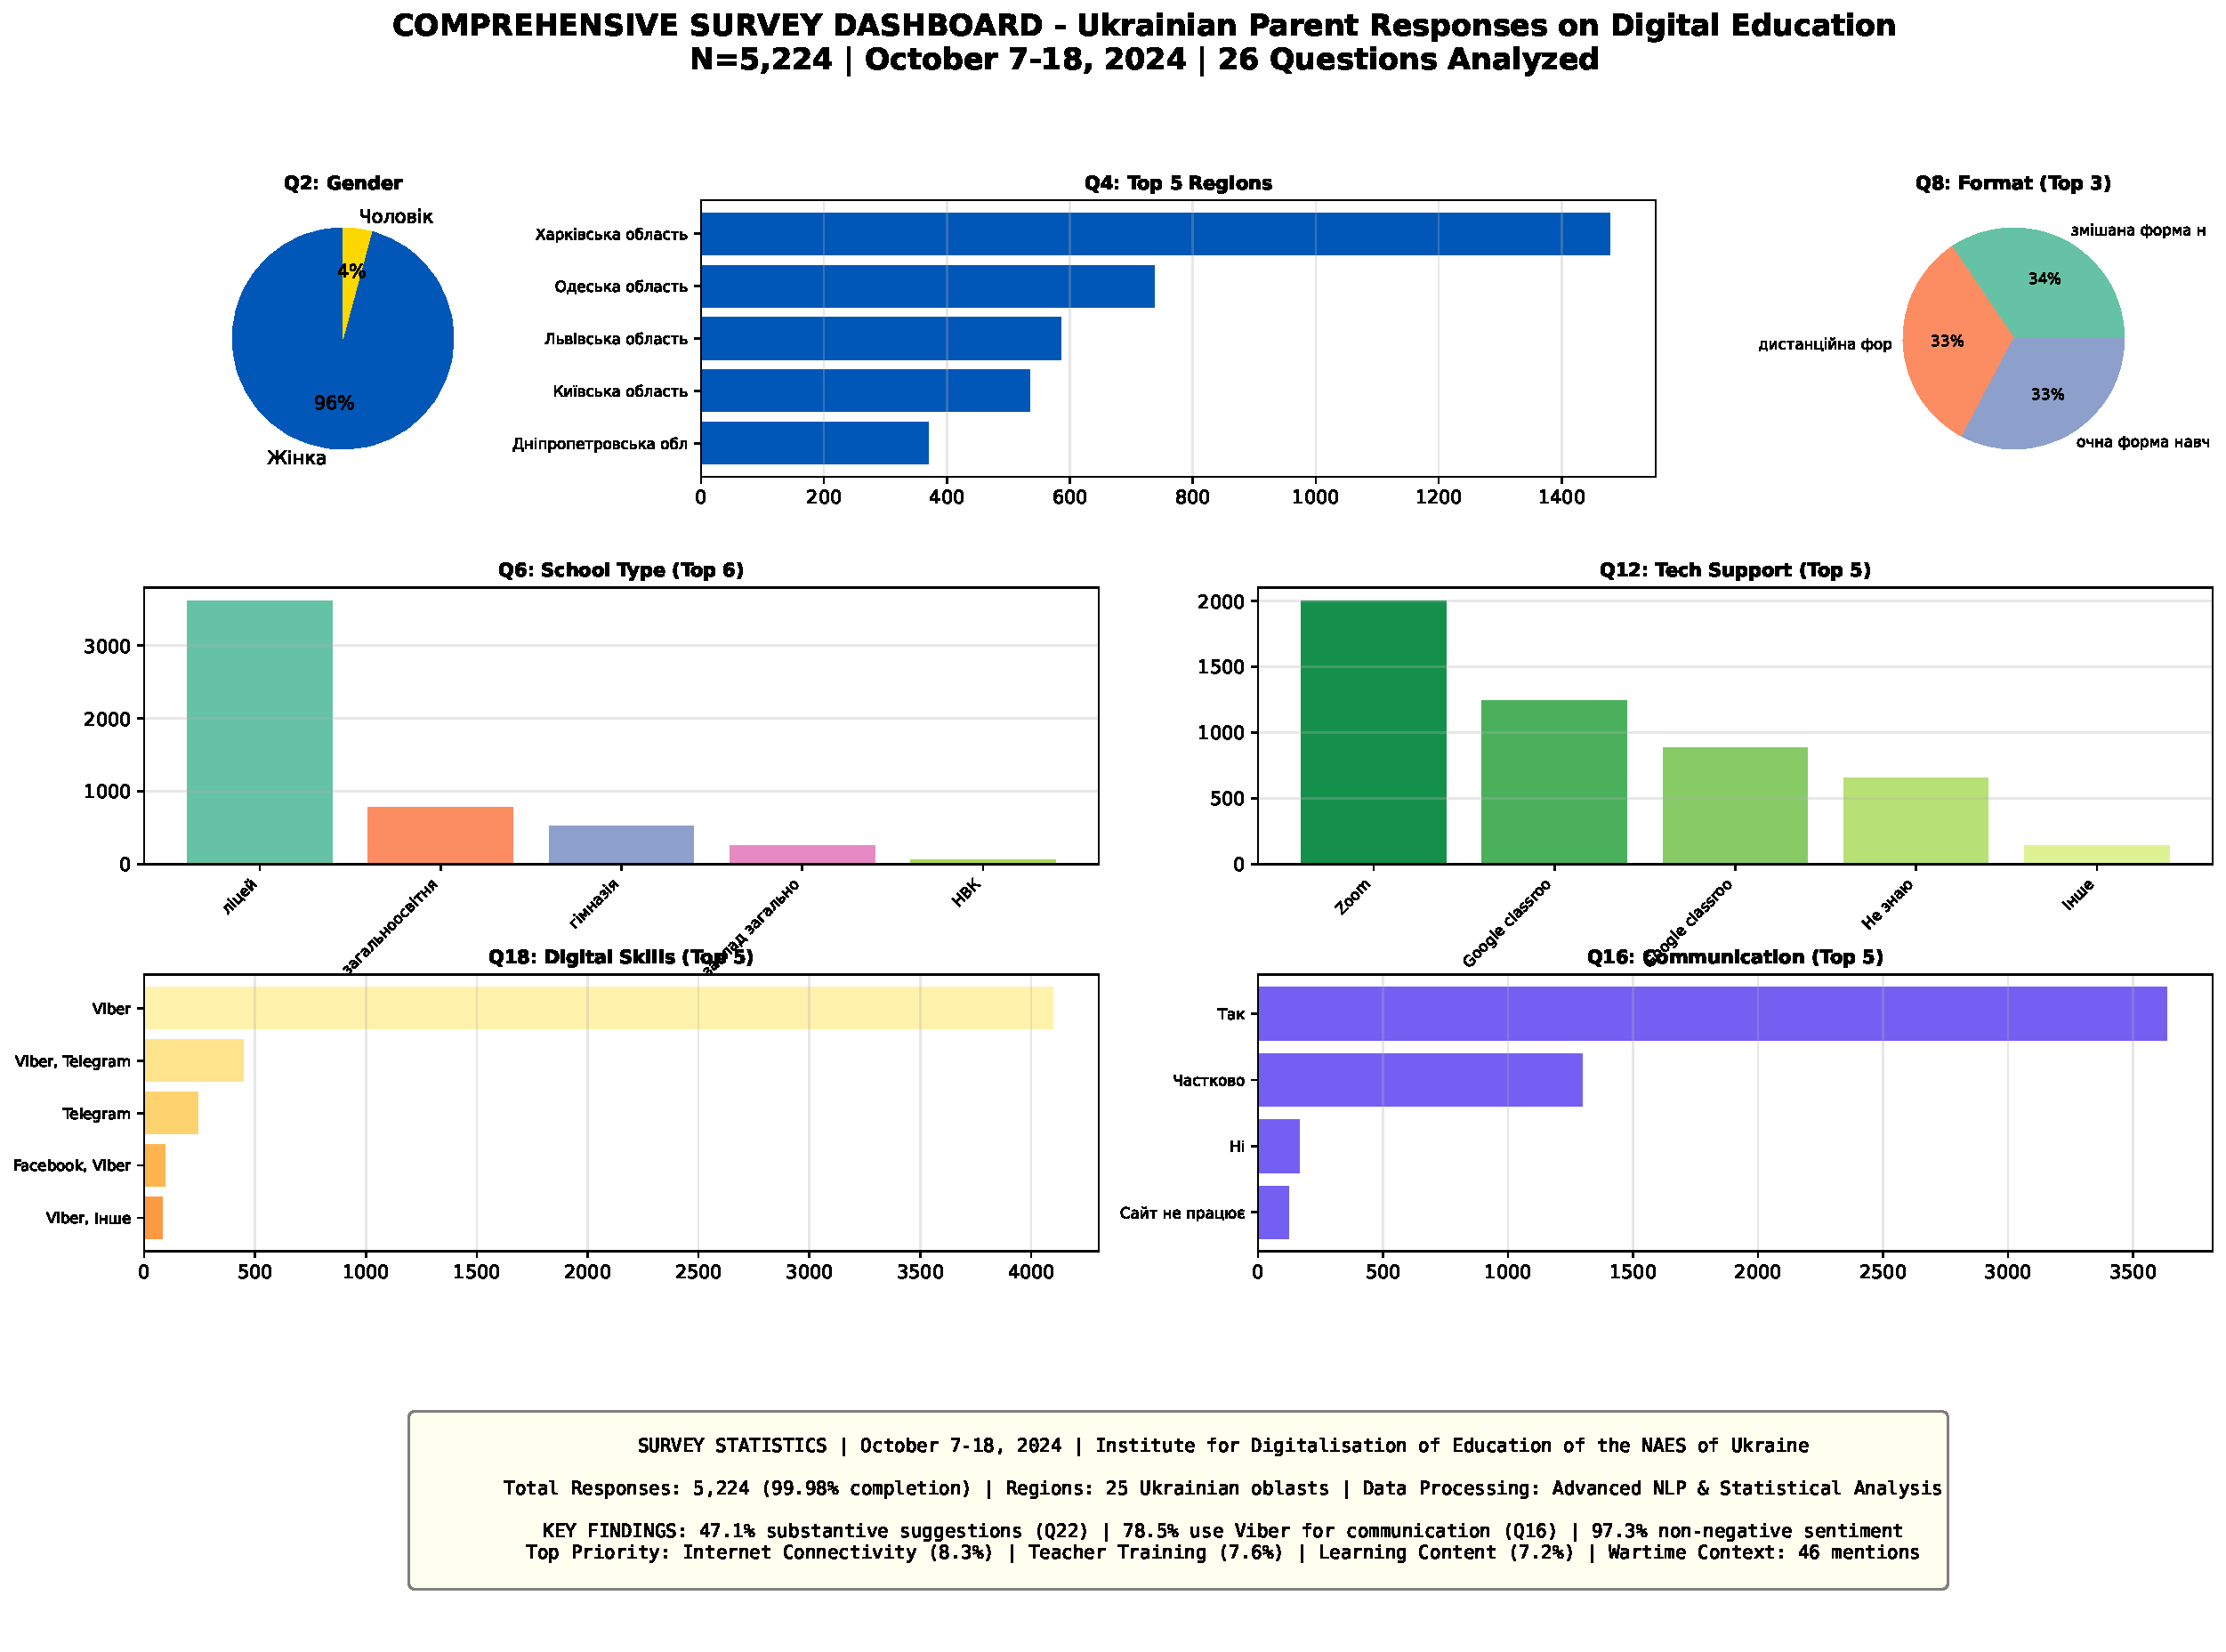
\includegraphics[width=\textwidth,height=0.85\textheight,keepaspectratio]{../visualizations/all_questions/complete_survey_dashboard.pdf}
    \caption{Complete Survey Dashboard - Overview of all 26 questions with key statistics and distributions across demographics, infrastructure, and satisfaction metrics.}
    \label{fig:complete_dashboard}
\end{figure}

\begin{figure}[H]
    \centering
    \includegraphics[width=\textwidth,height=0.85\textheight,keepaspectratio]{../visualizations/all_questions/response_quality_overview.pdf}
    \caption{Response Quality and Completeness Analysis - Missing data patterns, response completeness distribution, daily response rates during October 7-18, 2024, and survey structure by question type.}
    \label{fig:response_quality}
\end{figure}

\newpage

%===================================================================================
\section{Demographics (Q1-Q5)}
%===================================================================================

\subsection{Age and Gender Distribution}

\begin{figure}[H]
    \centering
    \begin{subfigure}[b]{0.48\textwidth}
        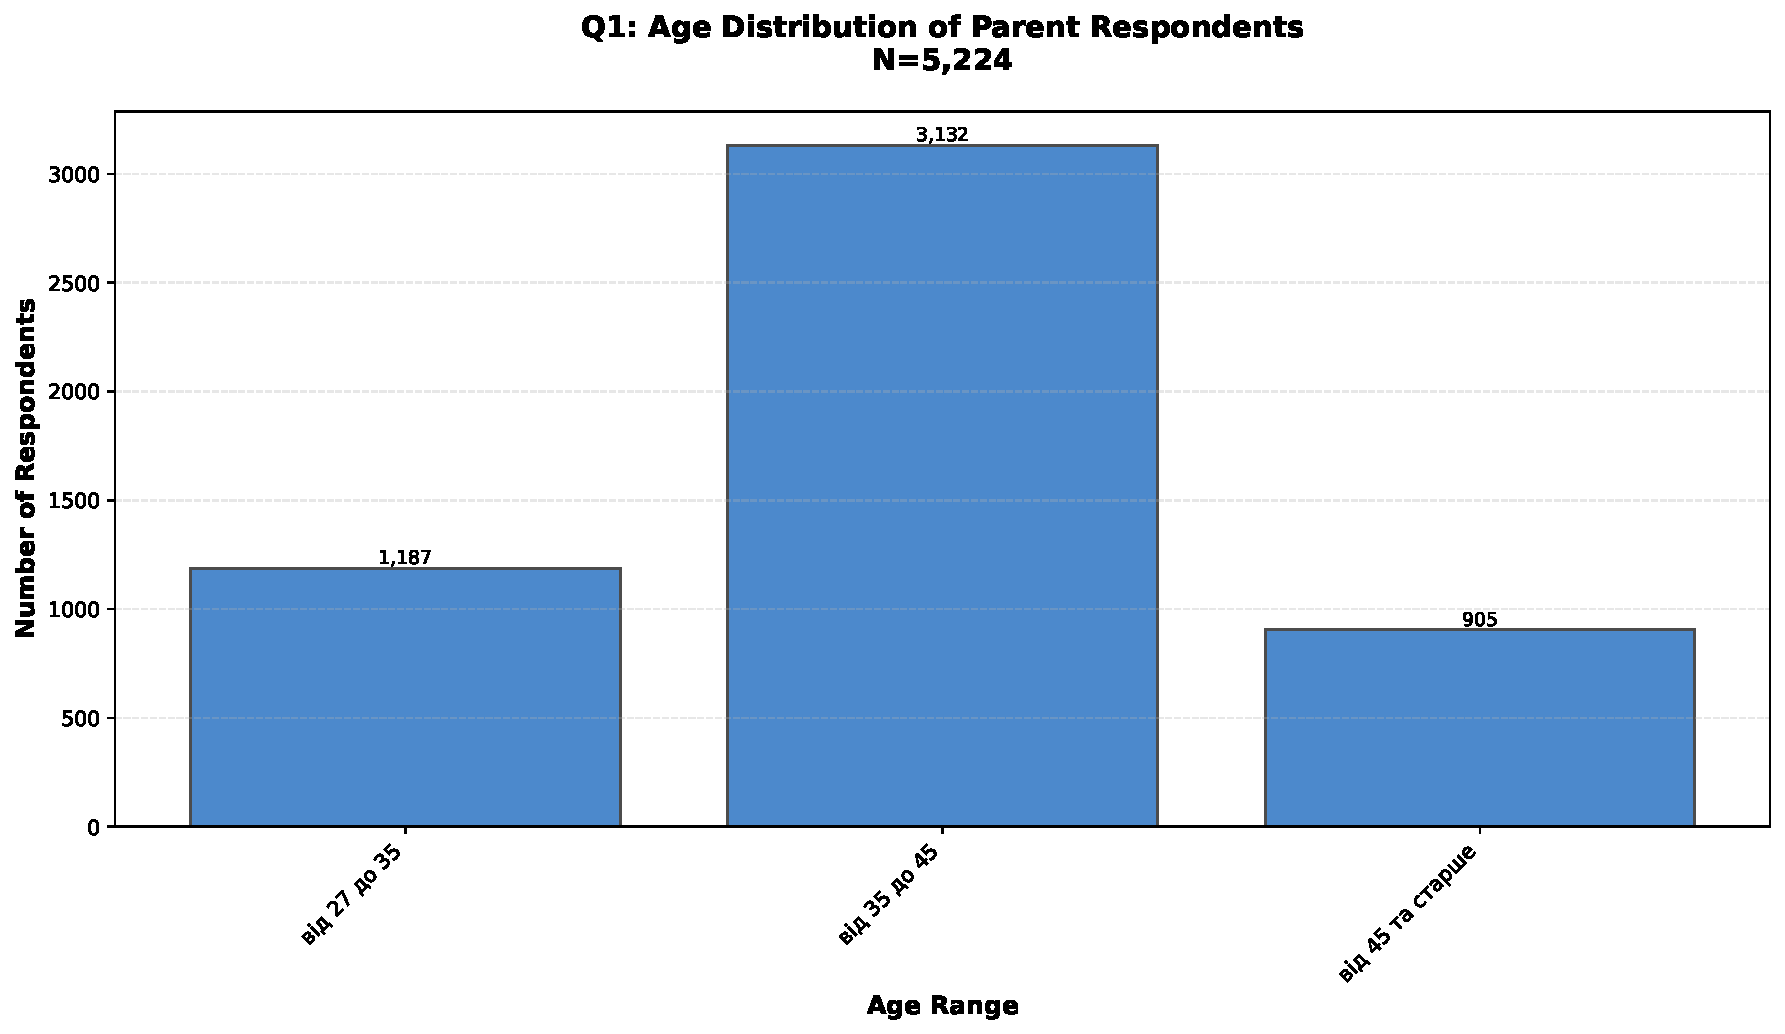
\includegraphics[width=\textwidth]{../visualizations/all_questions/q1_age_distribution.pdf}
        \caption{Q1: Age distribution of parent respondents}
        \label{fig:q1_age}
    \end{subfigure}
    \hfill
    \begin{subfigure}[b]{0.48\textwidth}
        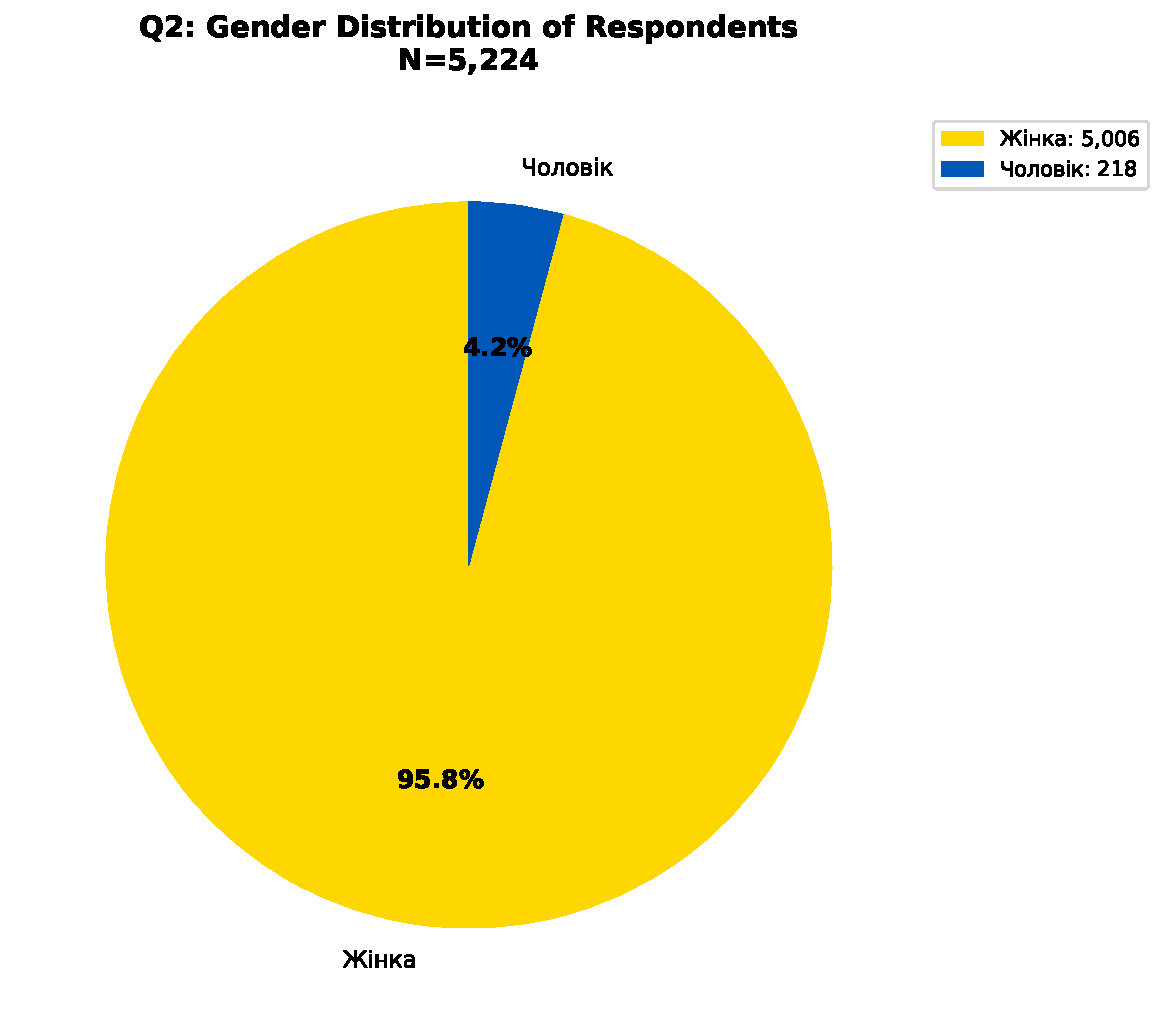
\includegraphics[width=\textwidth]{../visualizations/all_questions/q2_gender_distribution.pdf}
        \caption{Q2: Gender distribution}
        \label{fig:q2_gender}
    \end{subfigure}
    \caption{Respondent Demographics - Age ranges and gender distribution of survey participants.}
    \label{fig:demographics_age_gender}
\end{figure}

\subsection{Geographic and Settlement Distribution}

\begin{figure}[H]
    \centering
    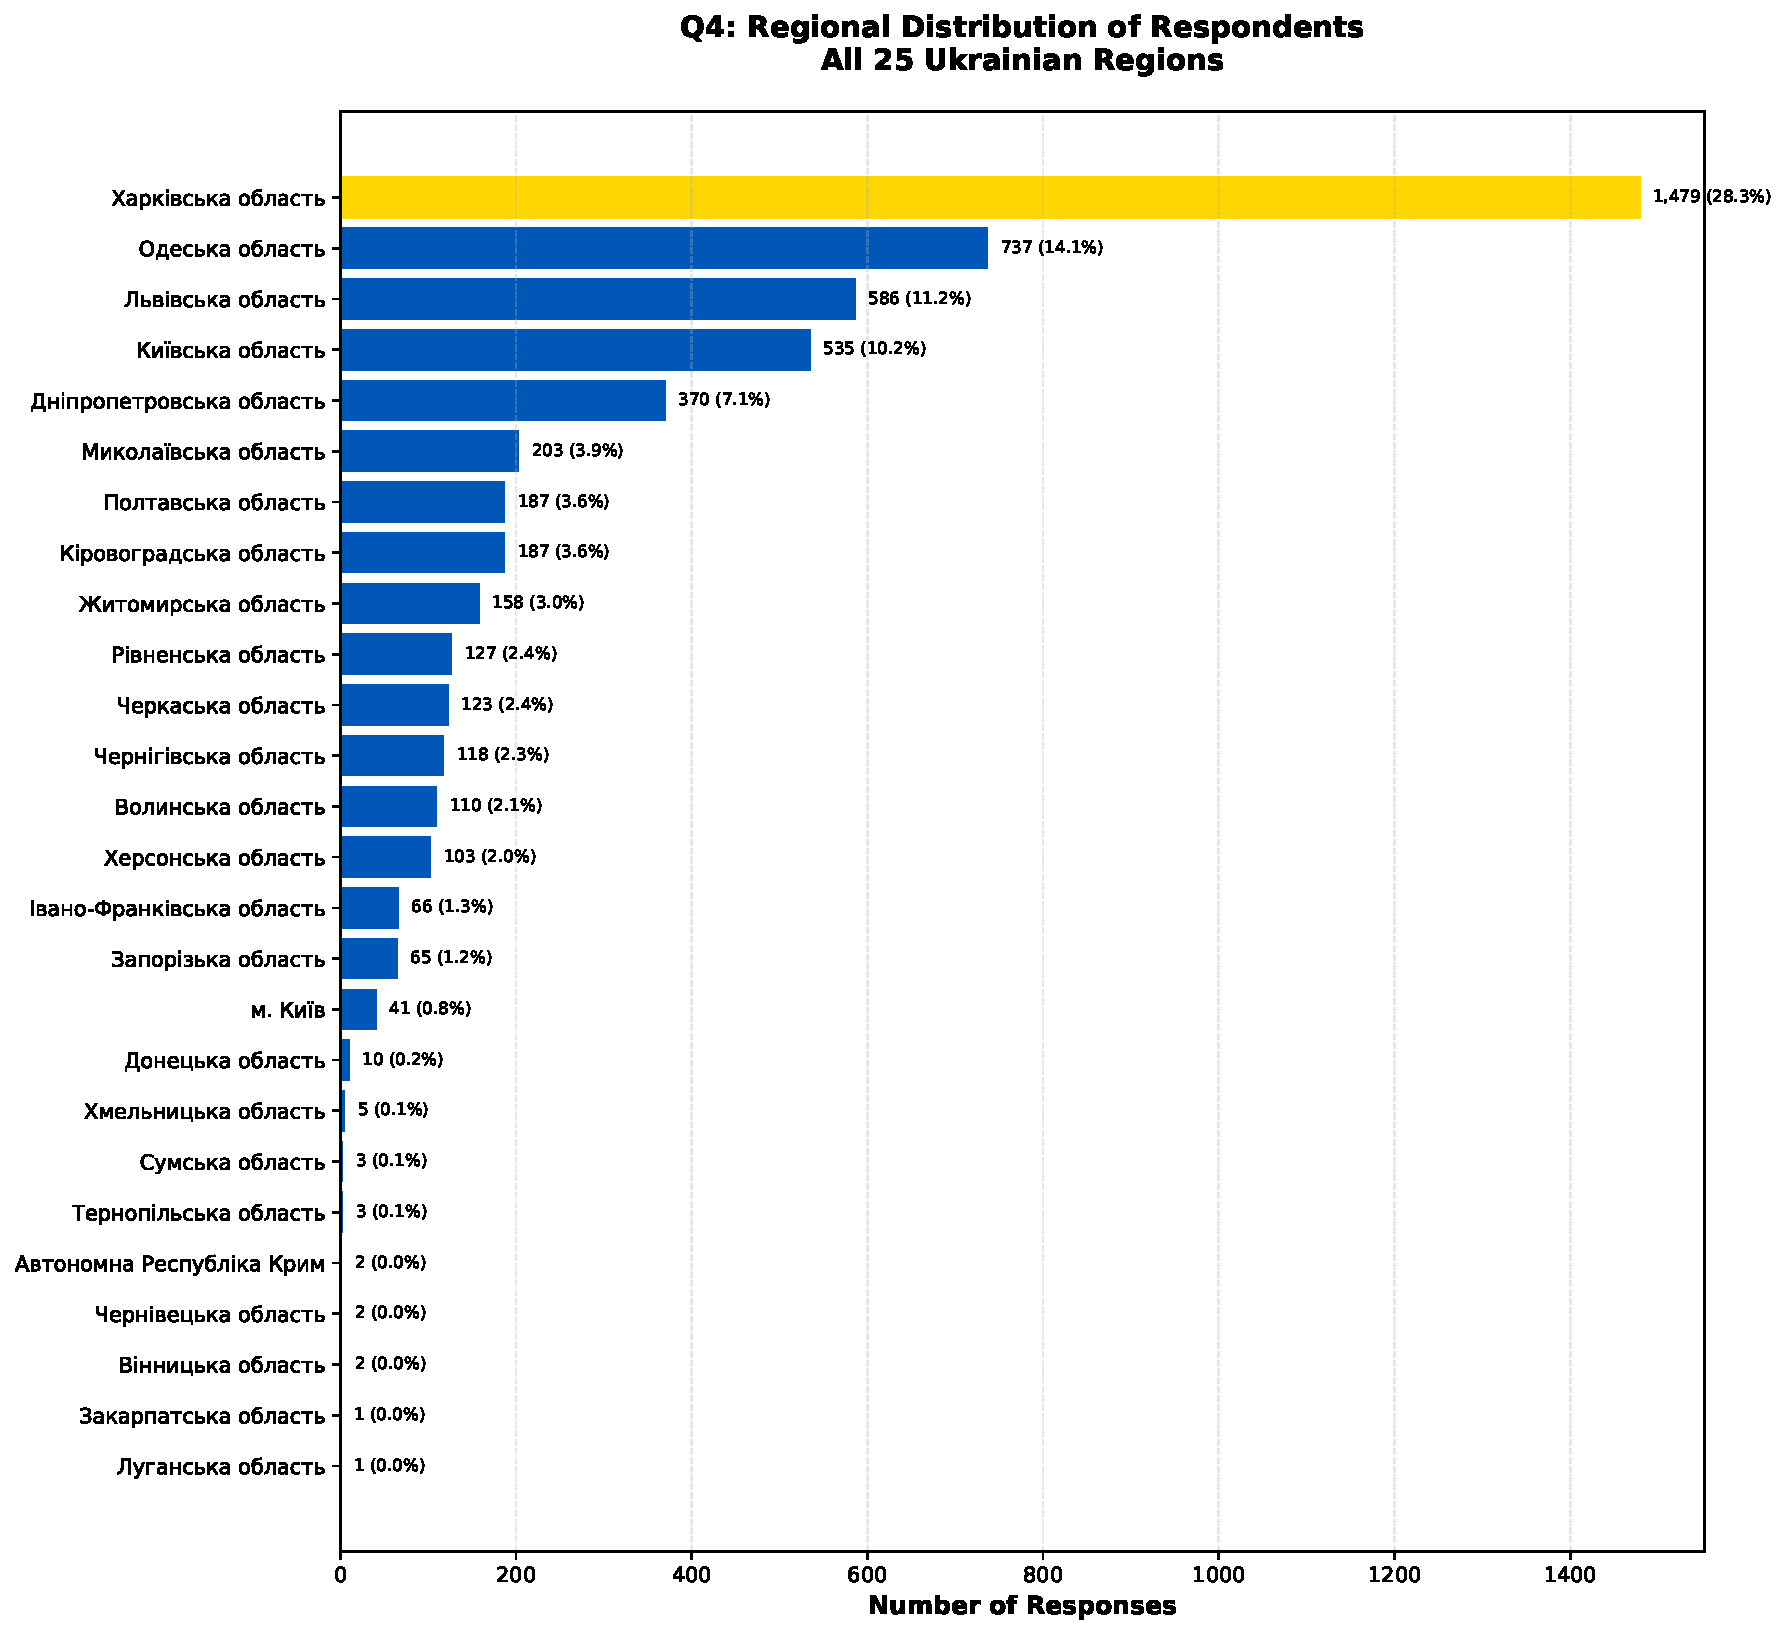
\includegraphics[width=\textwidth,height=0.9\textheight,keepaspectratio]{../visualizations/all_questions/q4_regional_distribution.pdf}
    \caption{Q4: Regional Distribution across all 25 Ukrainian Oblasts - Kharkiv Oblast leads with 28.3\% of responses, reflecting high engagement from frontline regions.}
    \label{fig:q4_regional}
\end{figure}

\begin{figure}[H]
    \centering
    \begin{subfigure}[b]{0.48\textwidth}
        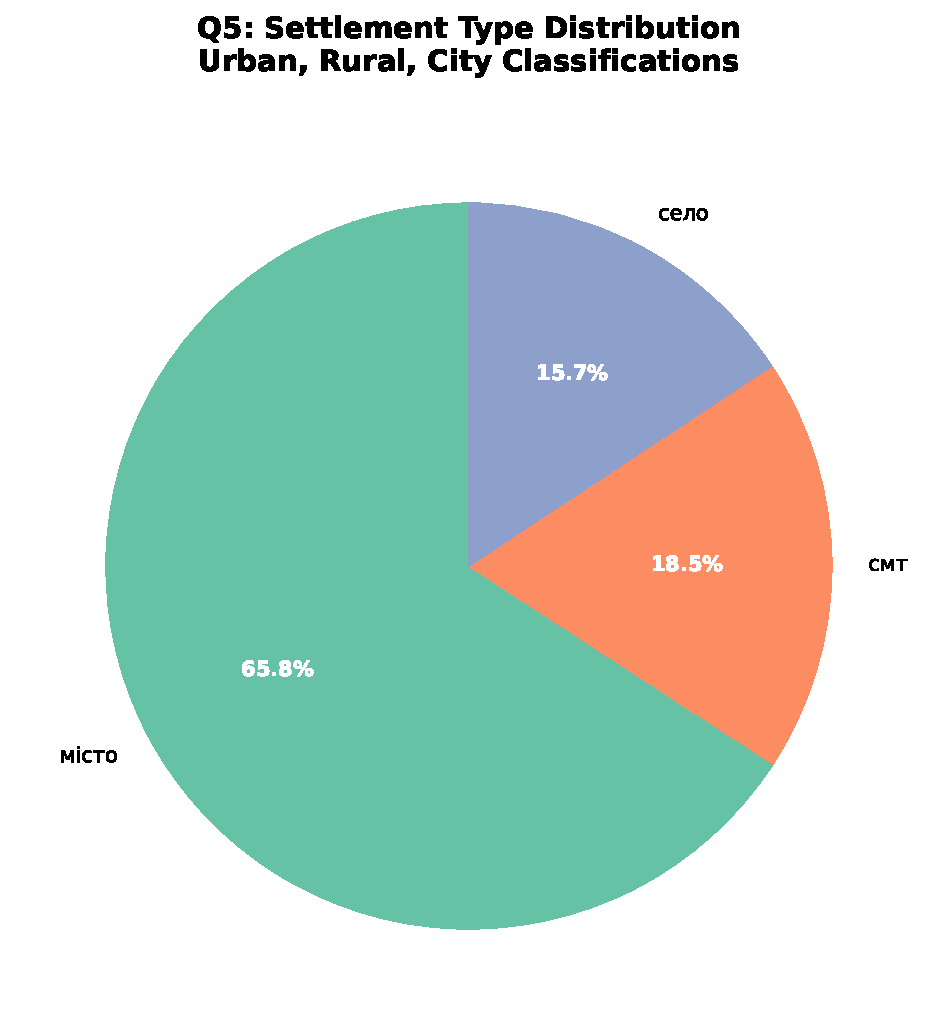
\includegraphics[width=\textwidth]{../visualizations/all_questions/q5_settlement_type.pdf}
        \caption{Q5: Settlement type (urban/rural/city classifications)}
        \label{fig:q5_settlement}
    \end{subfigure}
    \hfill
    \begin{subfigure}[b]{0.48\textwidth}
        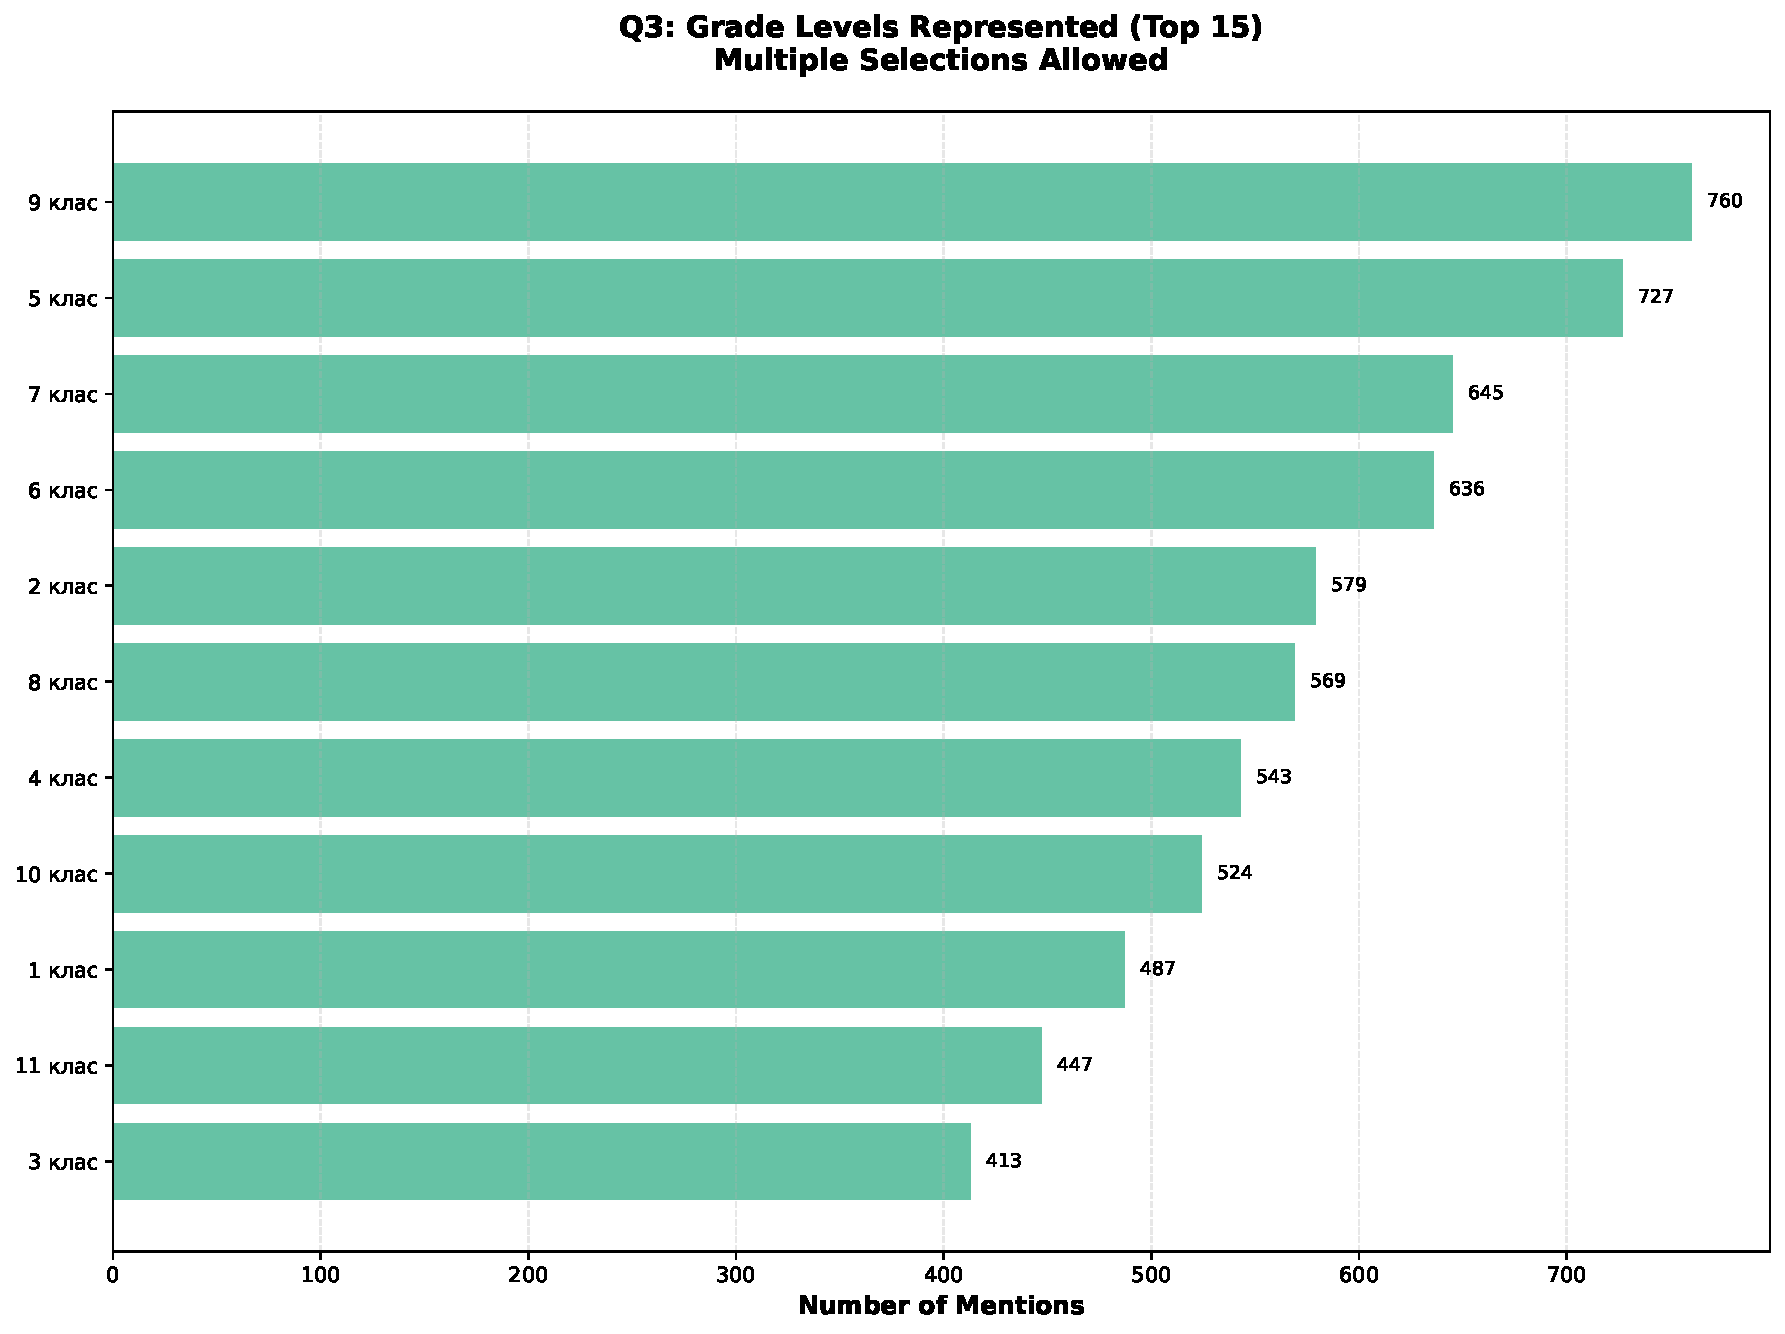
\includegraphics[width=\textwidth]{../visualizations/all_questions/q3_grade_levels.pdf}
        \caption{Q3: Grade levels represented (multiple selections allowed)}
        \label{fig:q3_grades}
    \end{subfigure}
    \caption{Geographic Distribution and Grade Levels - Settlement types and educational grade distribution across the sample.}
    \label{fig:geo_grades}
\end{figure}

\newpage

%===================================================================================
\section{School Characteristics (Q6-Q9)}
%===================================================================================

\begin{figure}[H]
    \centering
    \begin{subfigure}[b]{0.48\textwidth}
        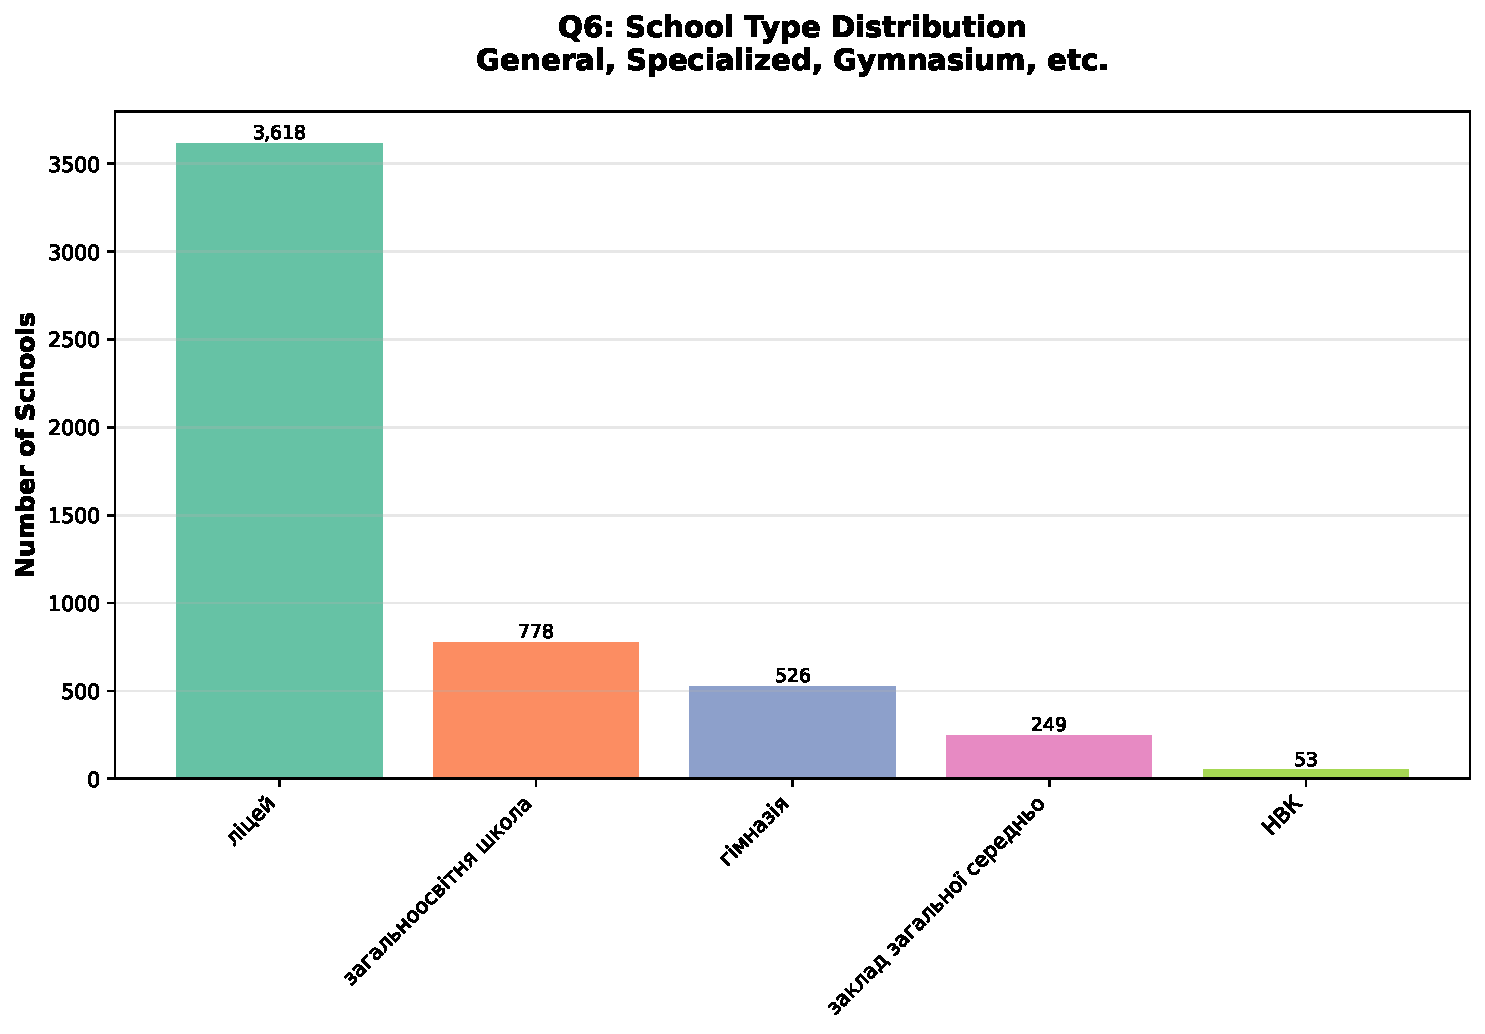
\includegraphics[width=\textwidth]{../visualizations/all_questions/q6_school_type.pdf}
        \caption{Q6: School type distribution}
        \label{fig:q6_school_type}
    \end{subfigure}
    \hfill
    \begin{subfigure}[b]{0.48\textwidth}
        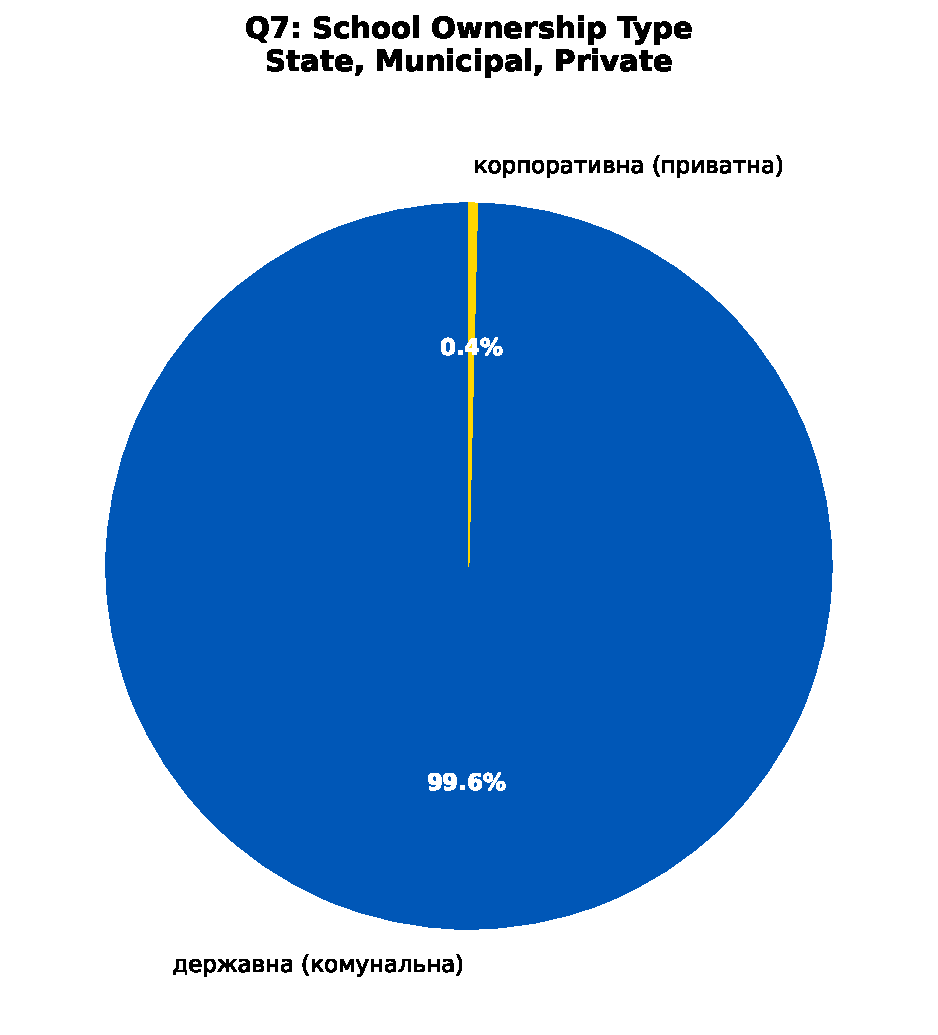
\includegraphics[width=\textwidth]{../visualizations/all_questions/q7_ownership.pdf}
        \caption{Q7: School ownership (state/municipal/private)}
        \label{fig:q7_ownership}
    \end{subfigure}
    \caption{School Types and Ownership - Distribution of general schools, specialized schools, gymnasiums, lyceums, and ownership models.}
    \label{fig:school_types}
\end{figure}

\begin{figure}[H]
    \centering
    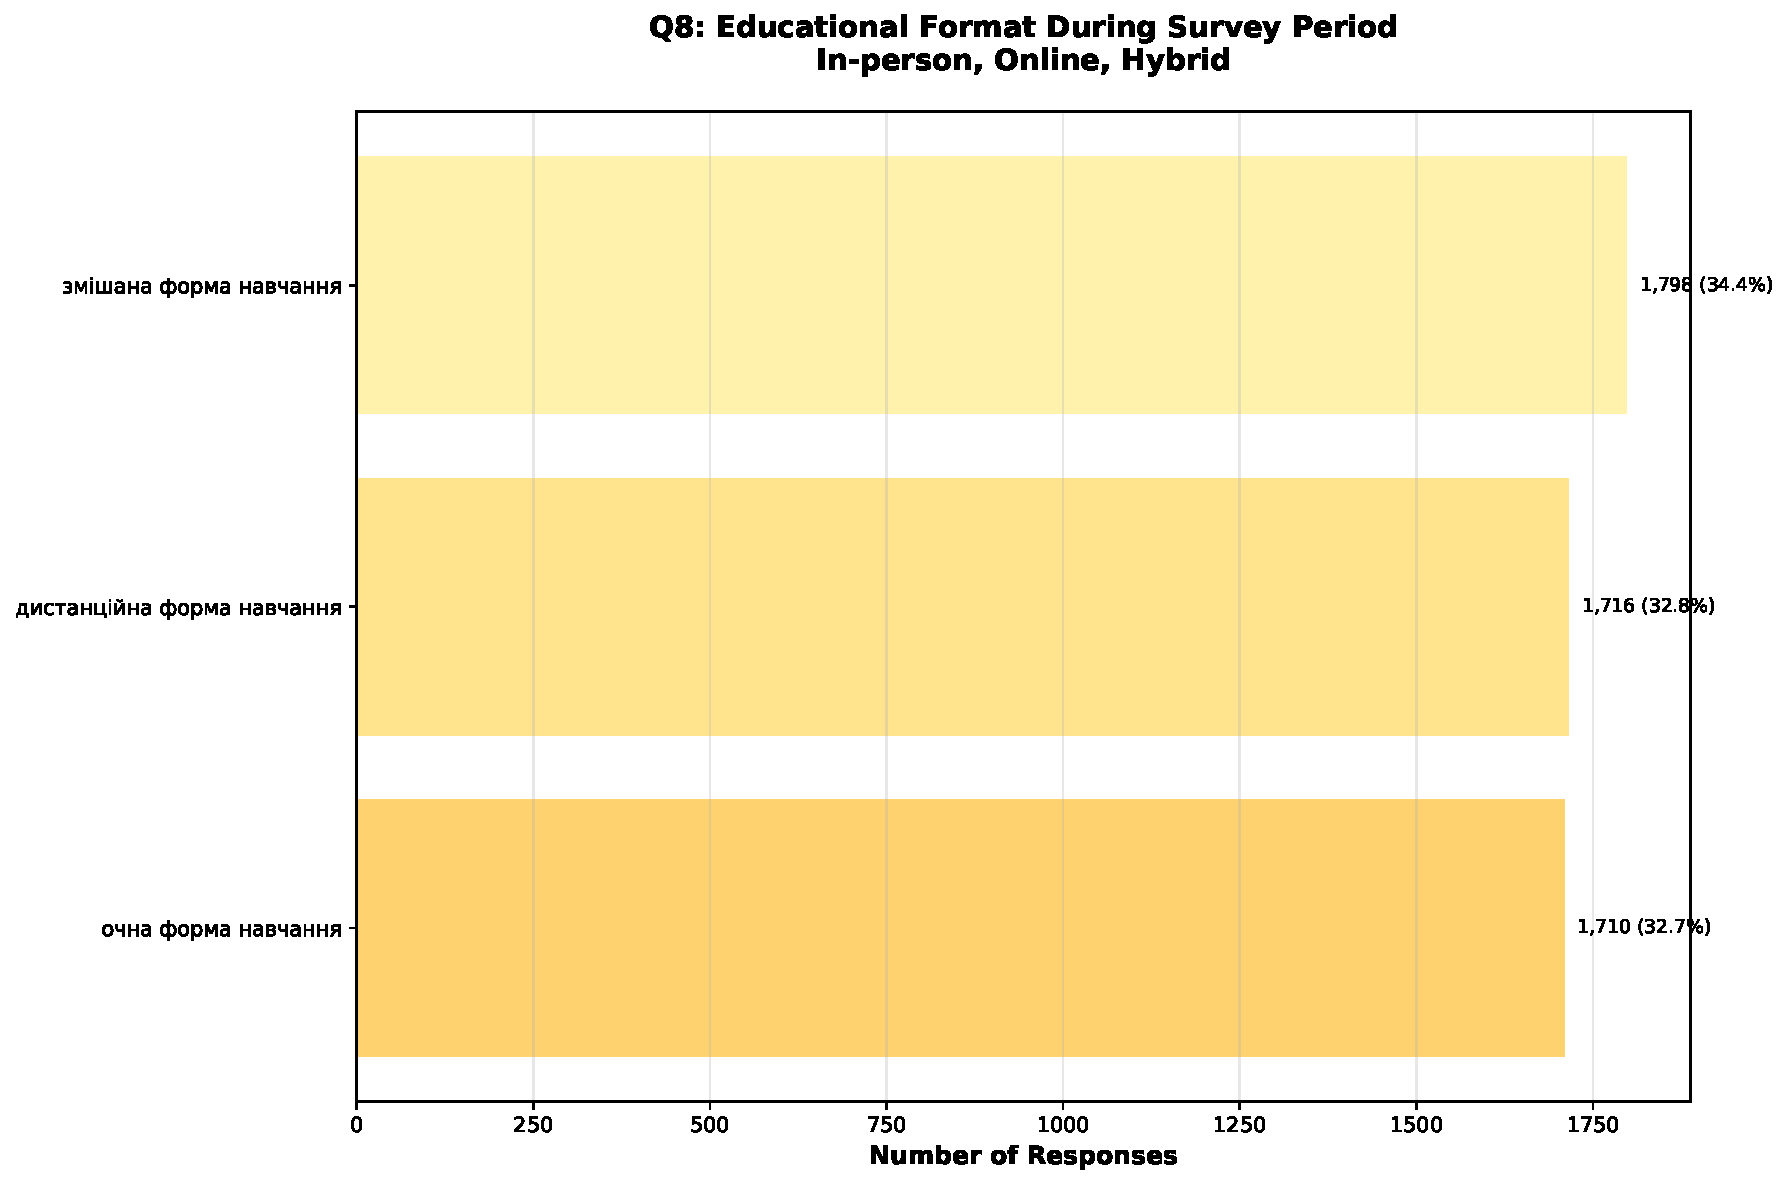
\includegraphics[width=\textwidth,height=0.8\textheight,keepaspectratio]{../visualizations/all_questions/q8_educational_format.pdf}
    \caption{Q8: Educational Format During Survey Period - In-person, online, hybrid, and mixed formats reflecting wartime adaptations.}
    \label{fig:q8_format}
\end{figure}

\begin{figure}[H]
    \centering
    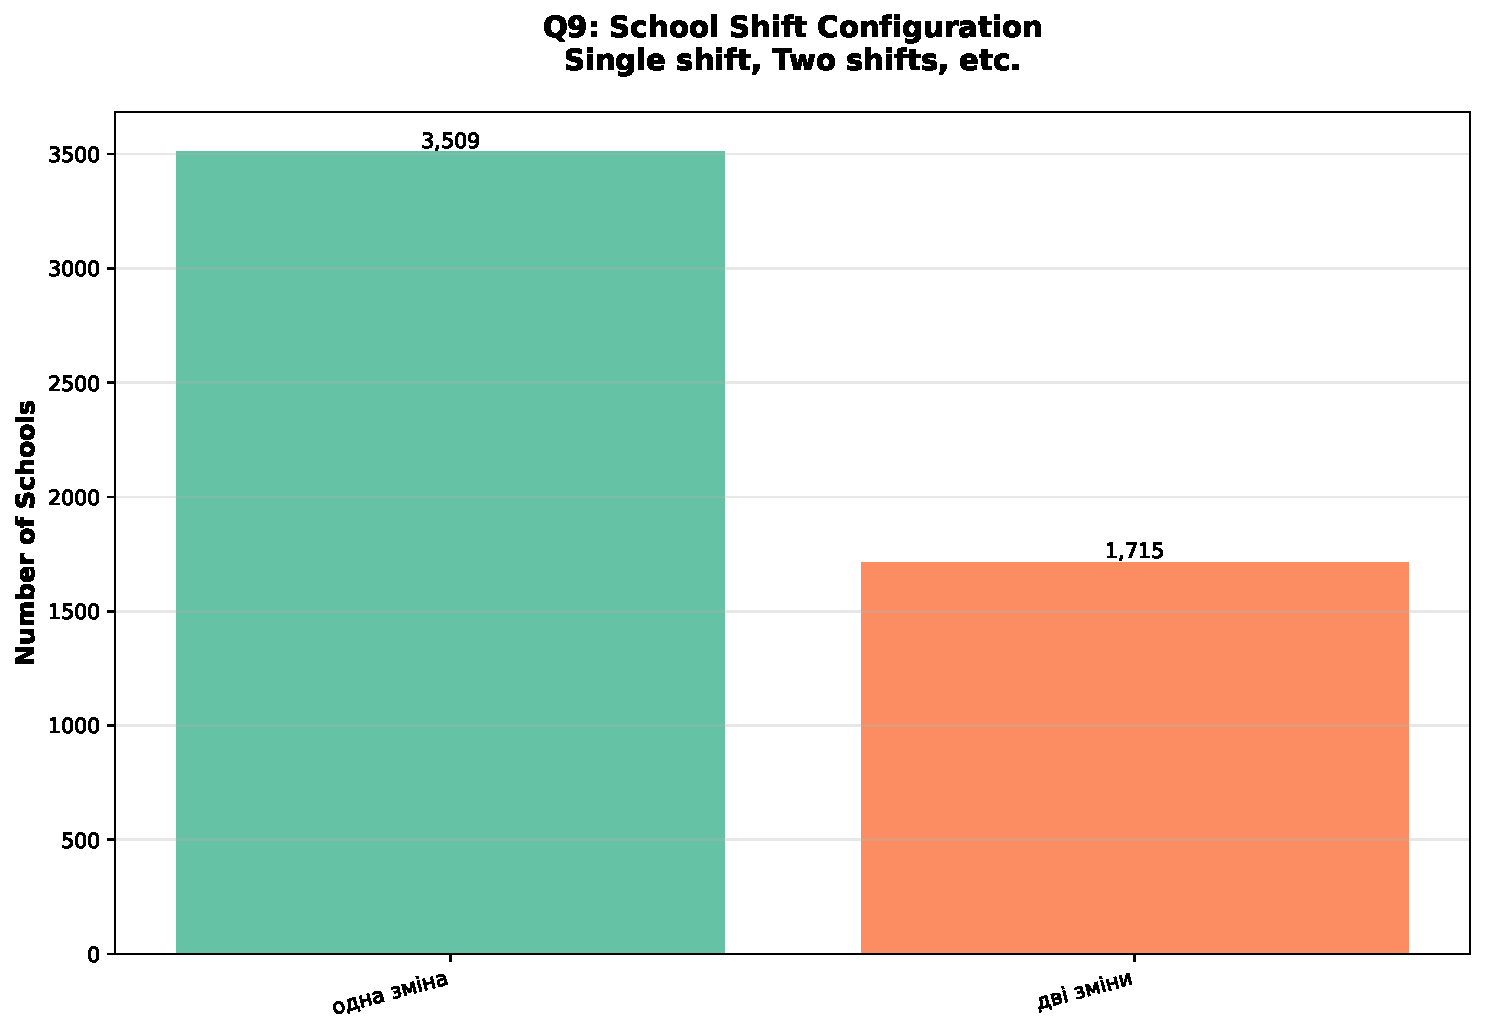
\includegraphics[width=0.7\textwidth]{../visualizations/all_questions/q9_school_shifts.pdf}
    \caption{Q9: School Shift Configuration - Single shift vs. multiple shift operations.}
    \label{fig:q9_shifts}
\end{figure}

\newpage

%===================================================================================
\section{Digital Infrastructure (Q10-Q11, Q16, Q21)}
%===================================================================================

\subsection{Platforms and Services}

\begin{figure}[H]
    \centering
    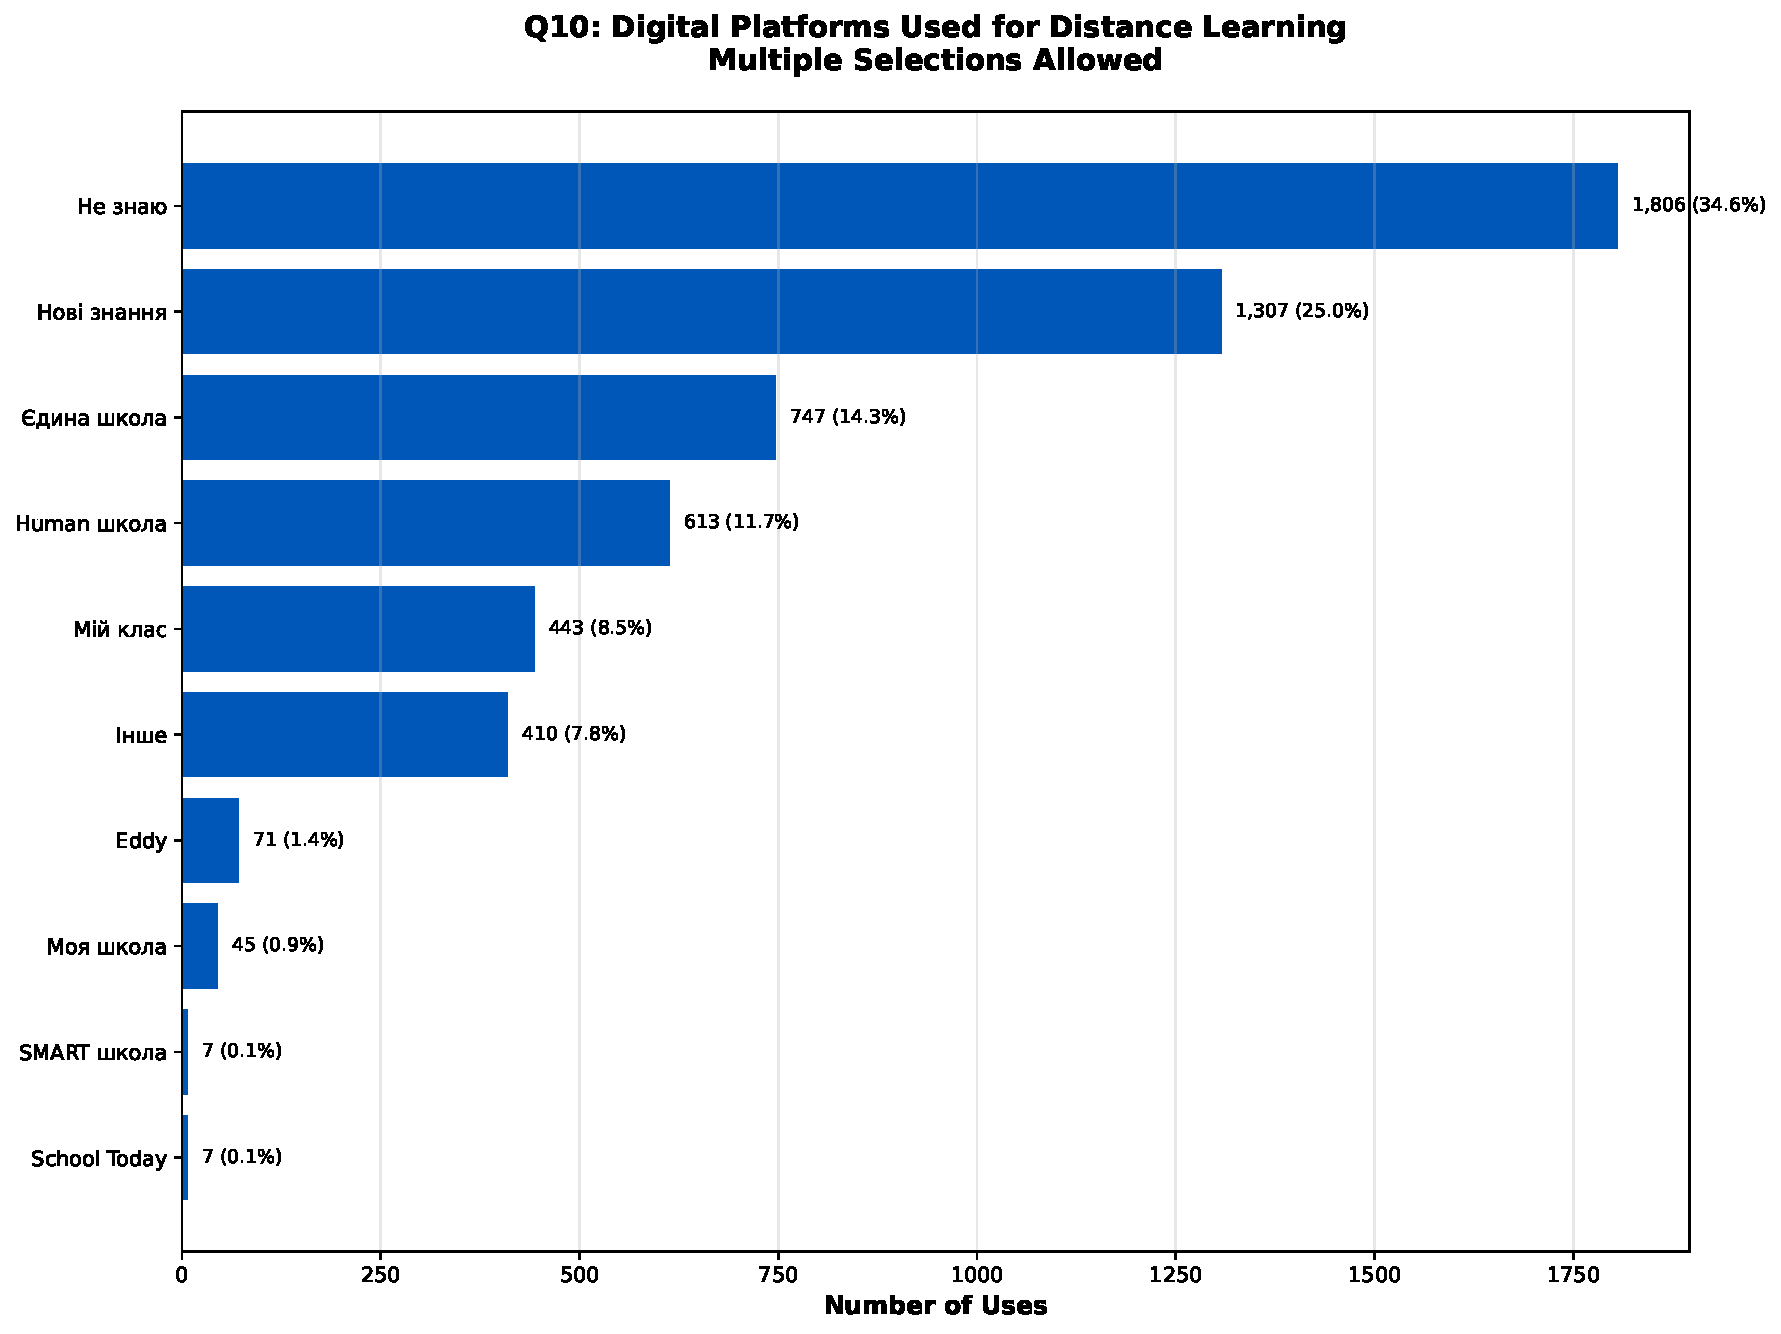
\includegraphics[width=\textwidth,height=0.85\textheight,keepaspectratio]{../visualizations/all_questions/q10_digital_platforms.pdf}
    \caption{Q10: Digital Platforms Used for Distance Learning - Zoom, Google Classroom, Microsoft Teams, and other platforms (multiple selections allowed).}
    \label{fig:q10_platforms}
\end{figure}

\begin{figure}[H]
    \centering
    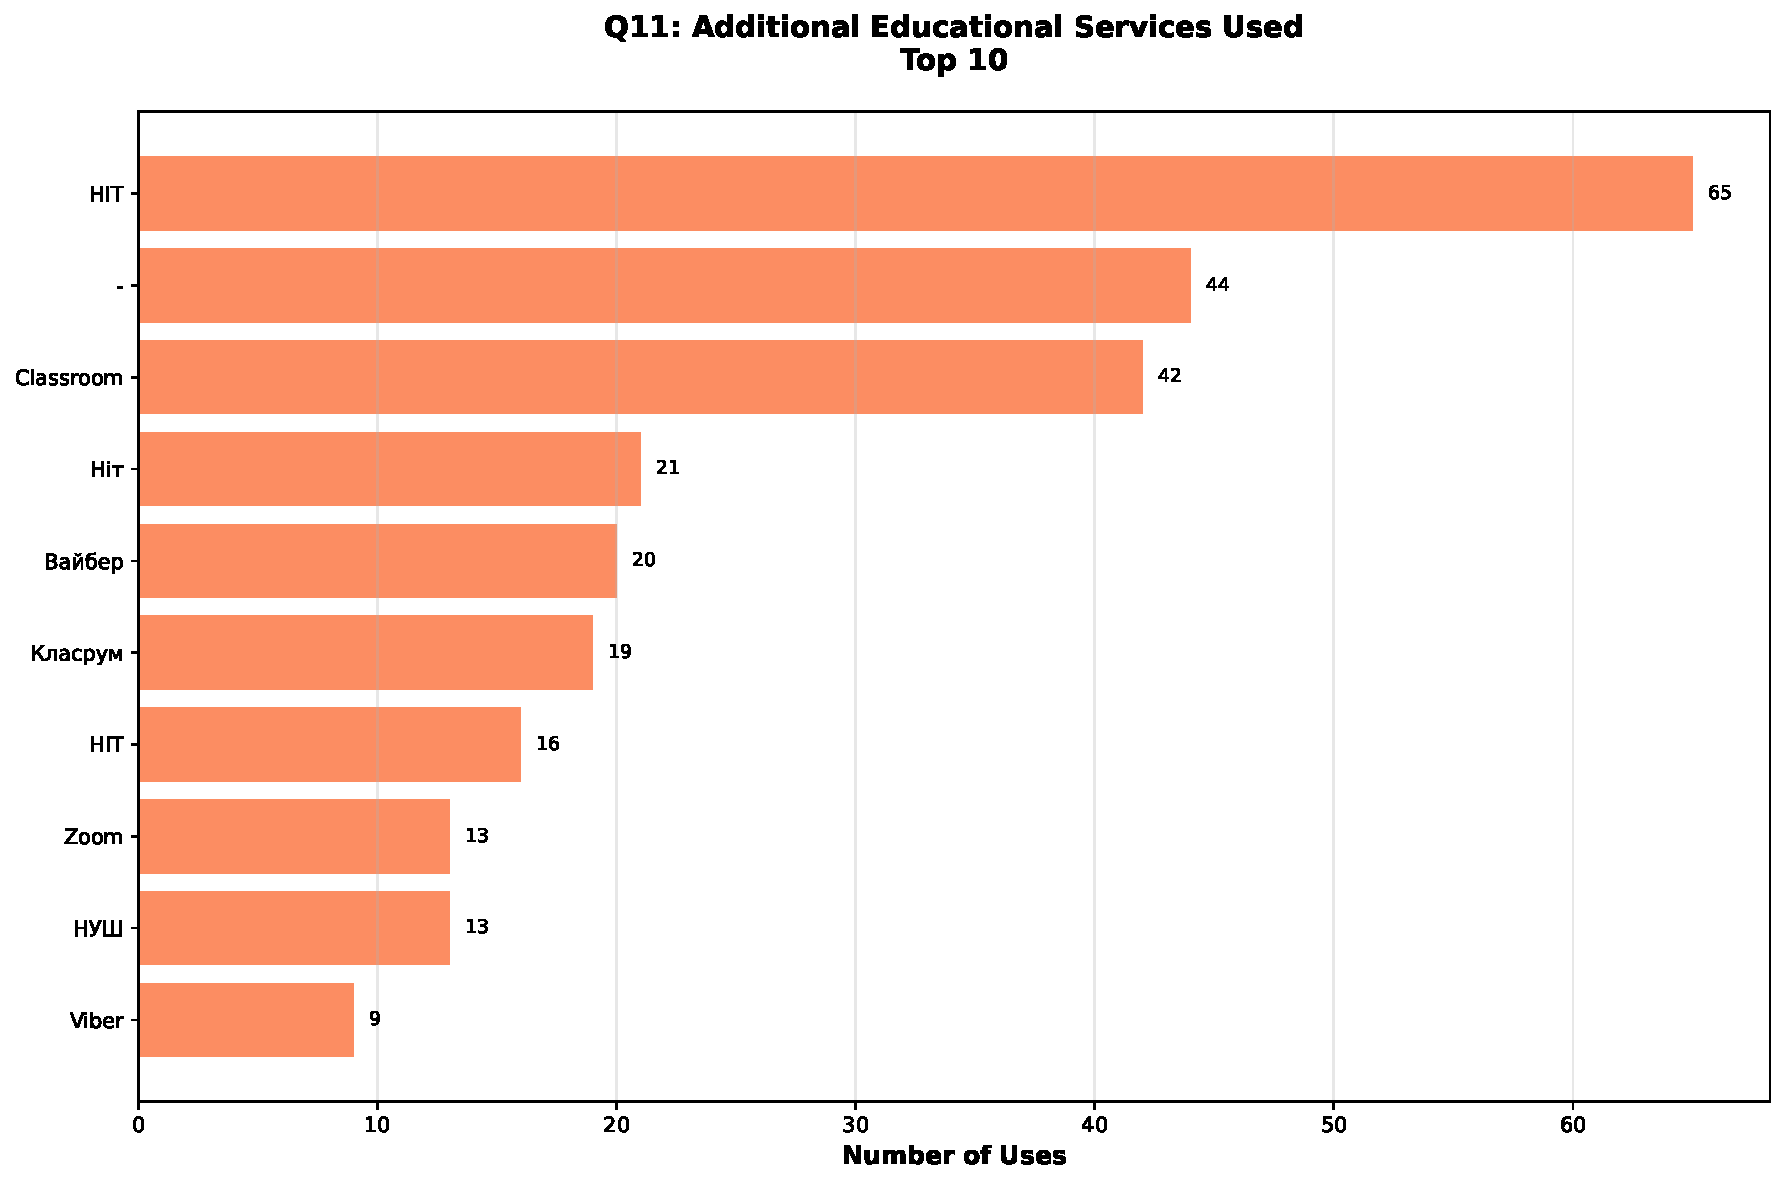
\includegraphics[width=\textwidth,height=0.8\textheight,keepaspectratio]{../visualizations/all_questions/q11_additional_services.pdf}
    \caption{Q11: Additional Educational Services Used - Supplementary platforms and tools for online education.}
    \label{fig:q11_services}
\end{figure}

\newpage

\subsection{Communication Channels and Device Access}

\begin{figure}[H]
    \centering
    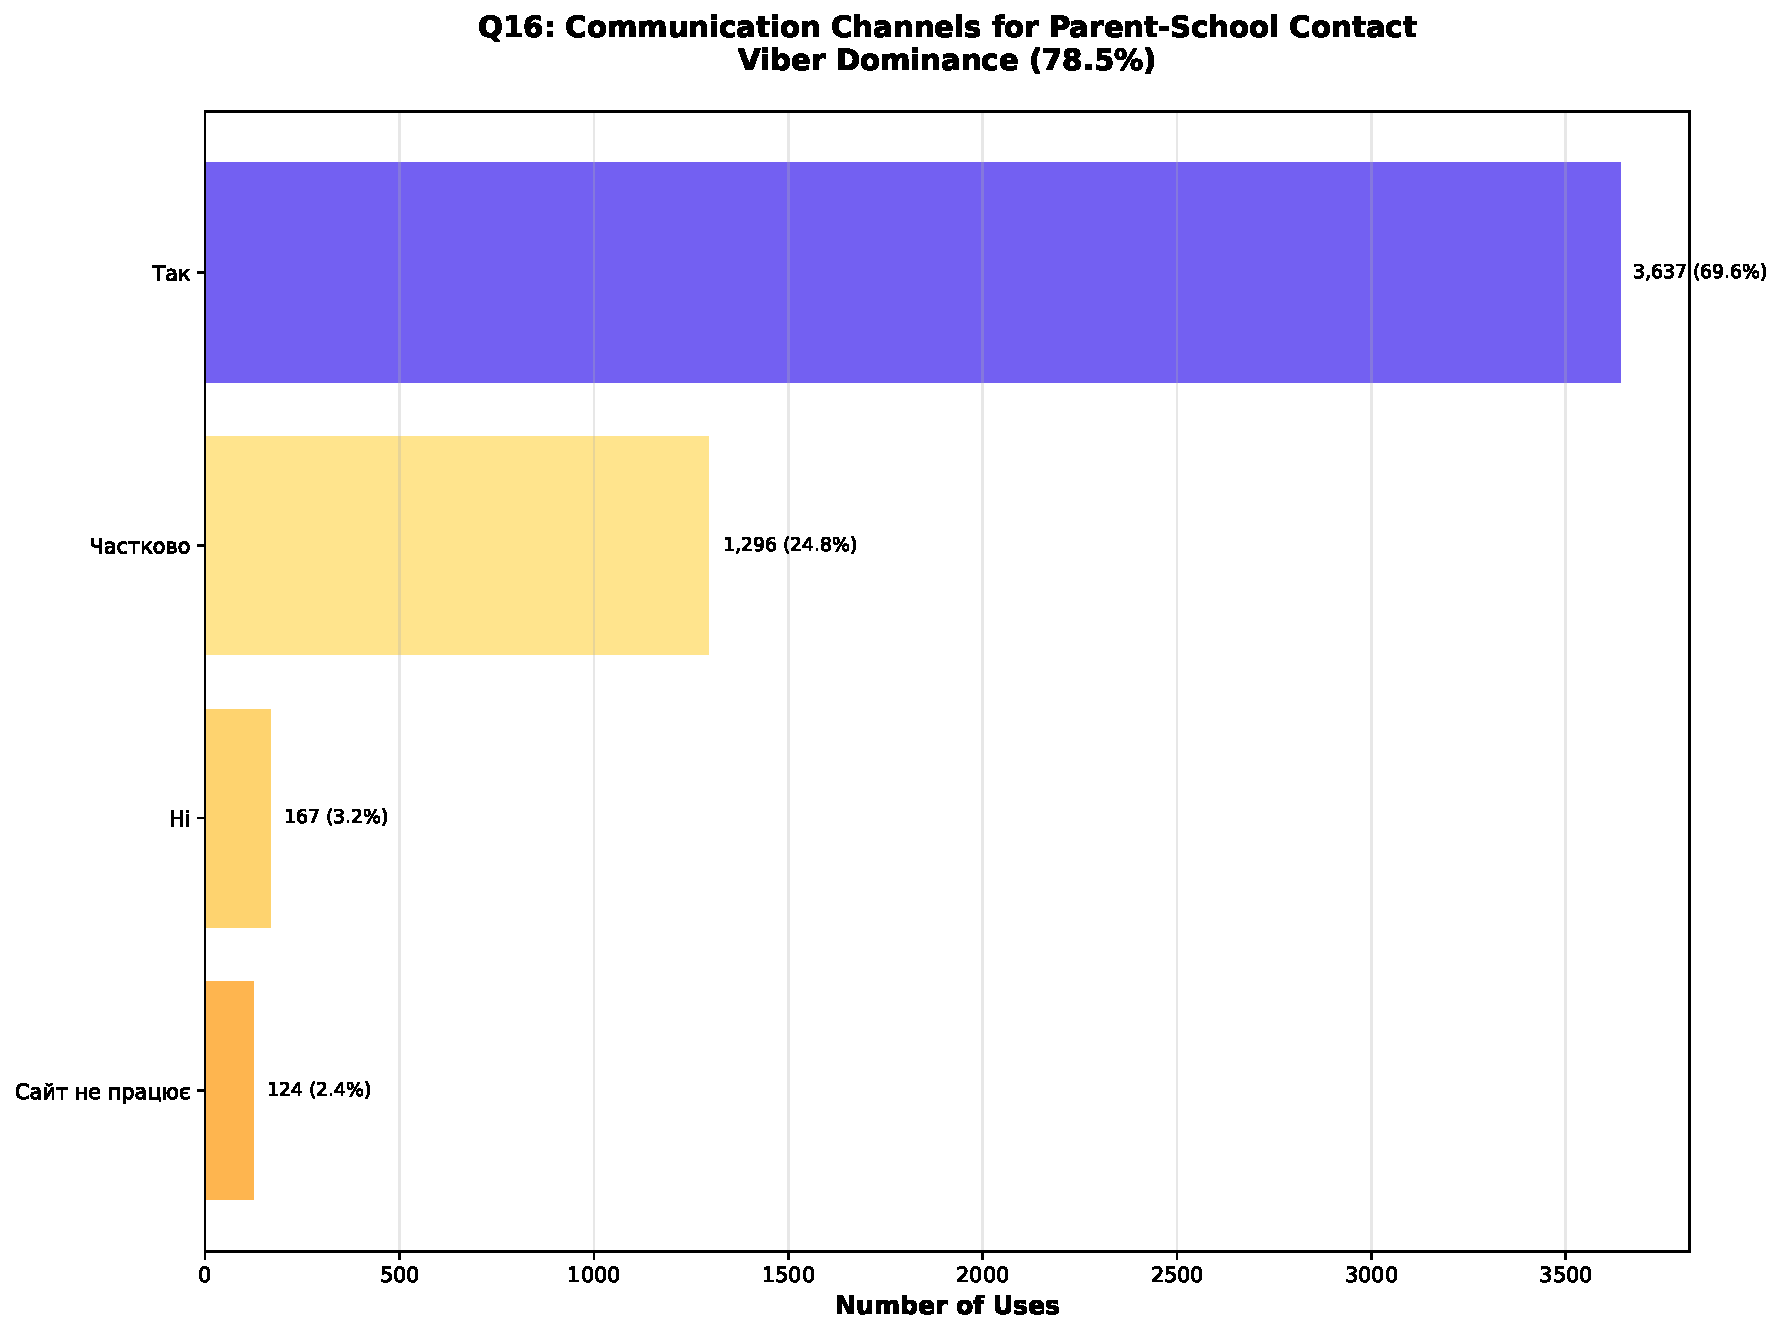
\includegraphics[width=\textwidth,height=0.9\textheight,keepaspectratio]{../visualizations/all_questions/q16_communication_channels.pdf}
    \caption{Q16: Communication Channels for Parent-School Contact - Viber dominates at 78.5\%, followed by Telegram, phone calls, and email (multiple selections allowed).}
    \label{fig:q16_communication}
\end{figure}

\begin{figure}[H]
    \centering
    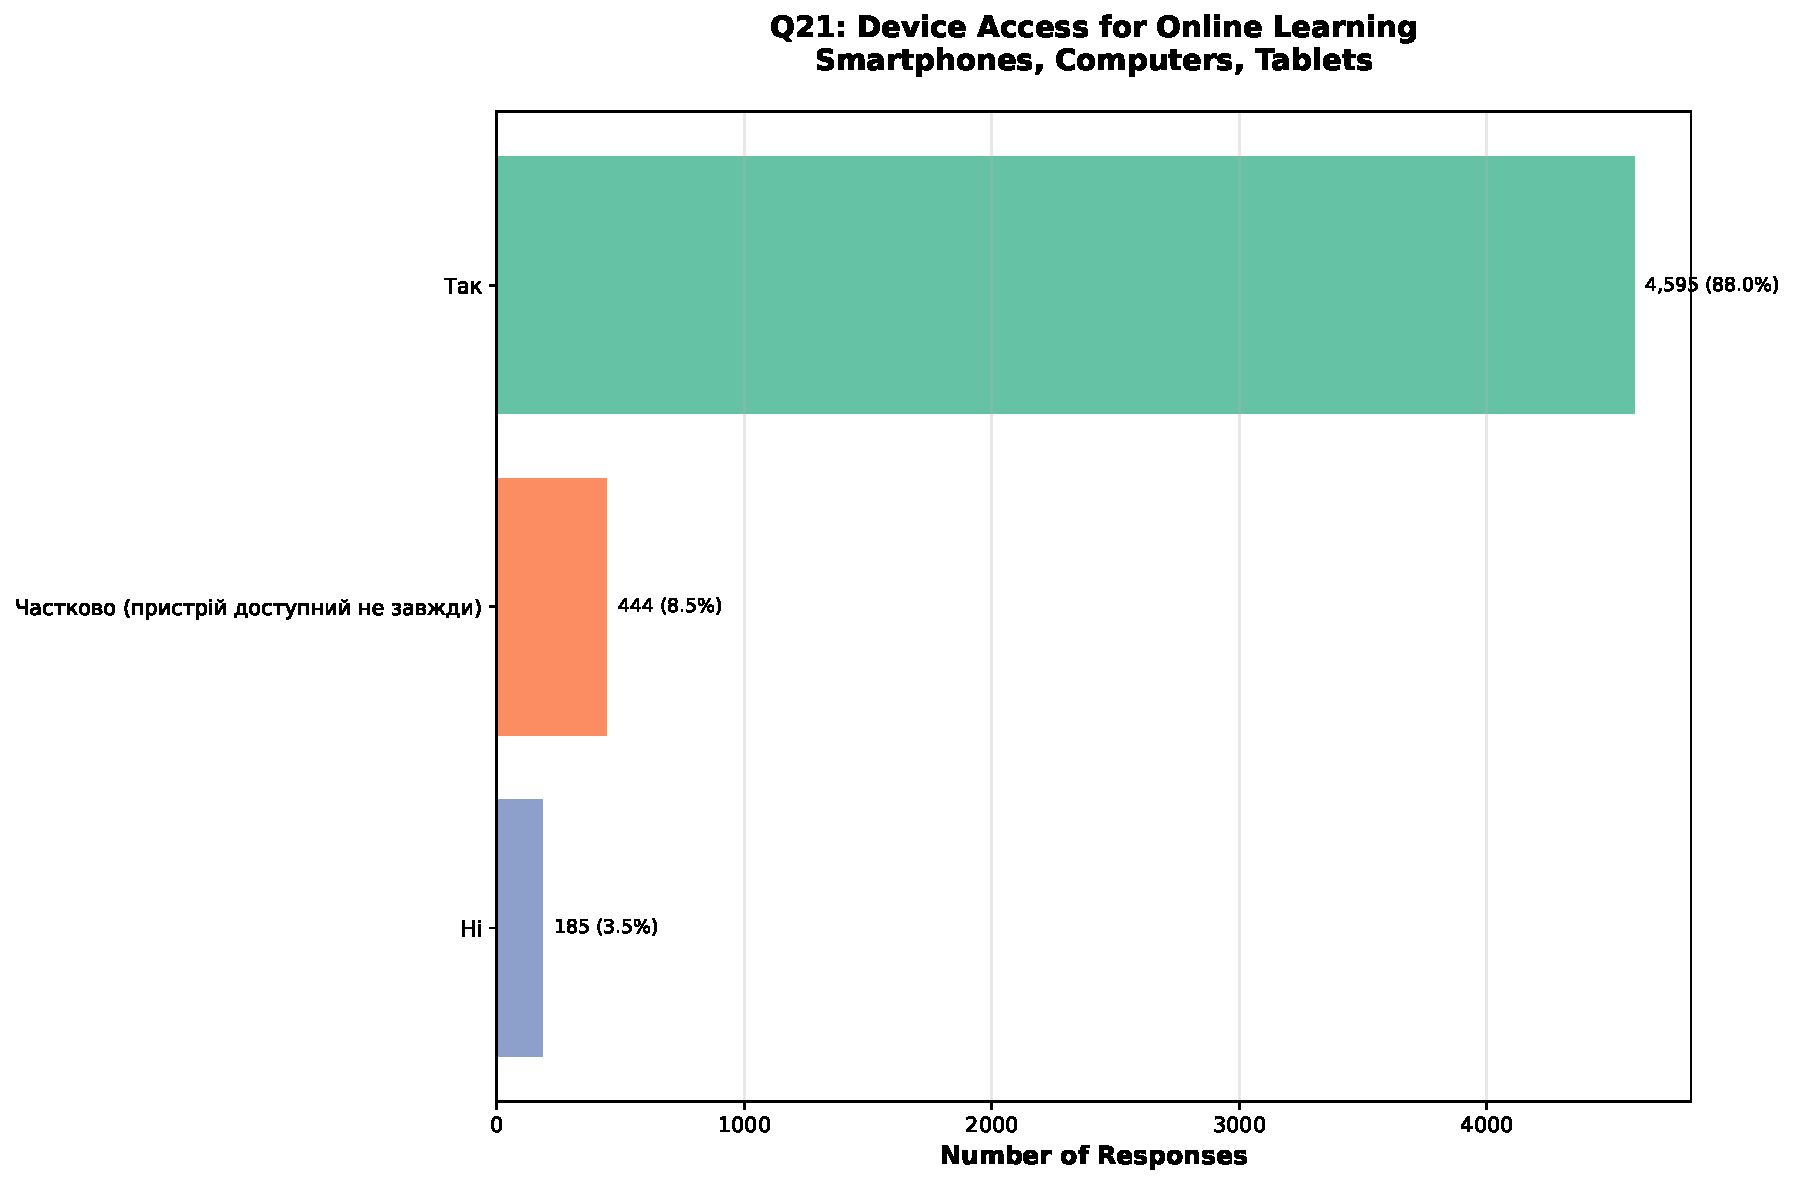
\includegraphics[width=\textwidth,height=0.8\textheight,keepaspectratio]{../visualizations/all_questions/q21_device_access.pdf}
    \caption{Q21: Device Access for Online Learning - Smartphones, computers, tablets, and other devices available to students.}
    \label{fig:q21_devices}
\end{figure}

\newpage

%===================================================================================
\section{Satisfaction \& Quality (Q12, Q14-Q15, Q17)}
%===================================================================================

\begin{figure}[H]
    \centering
    \begin{subfigure}[b]{0.48\textwidth}
        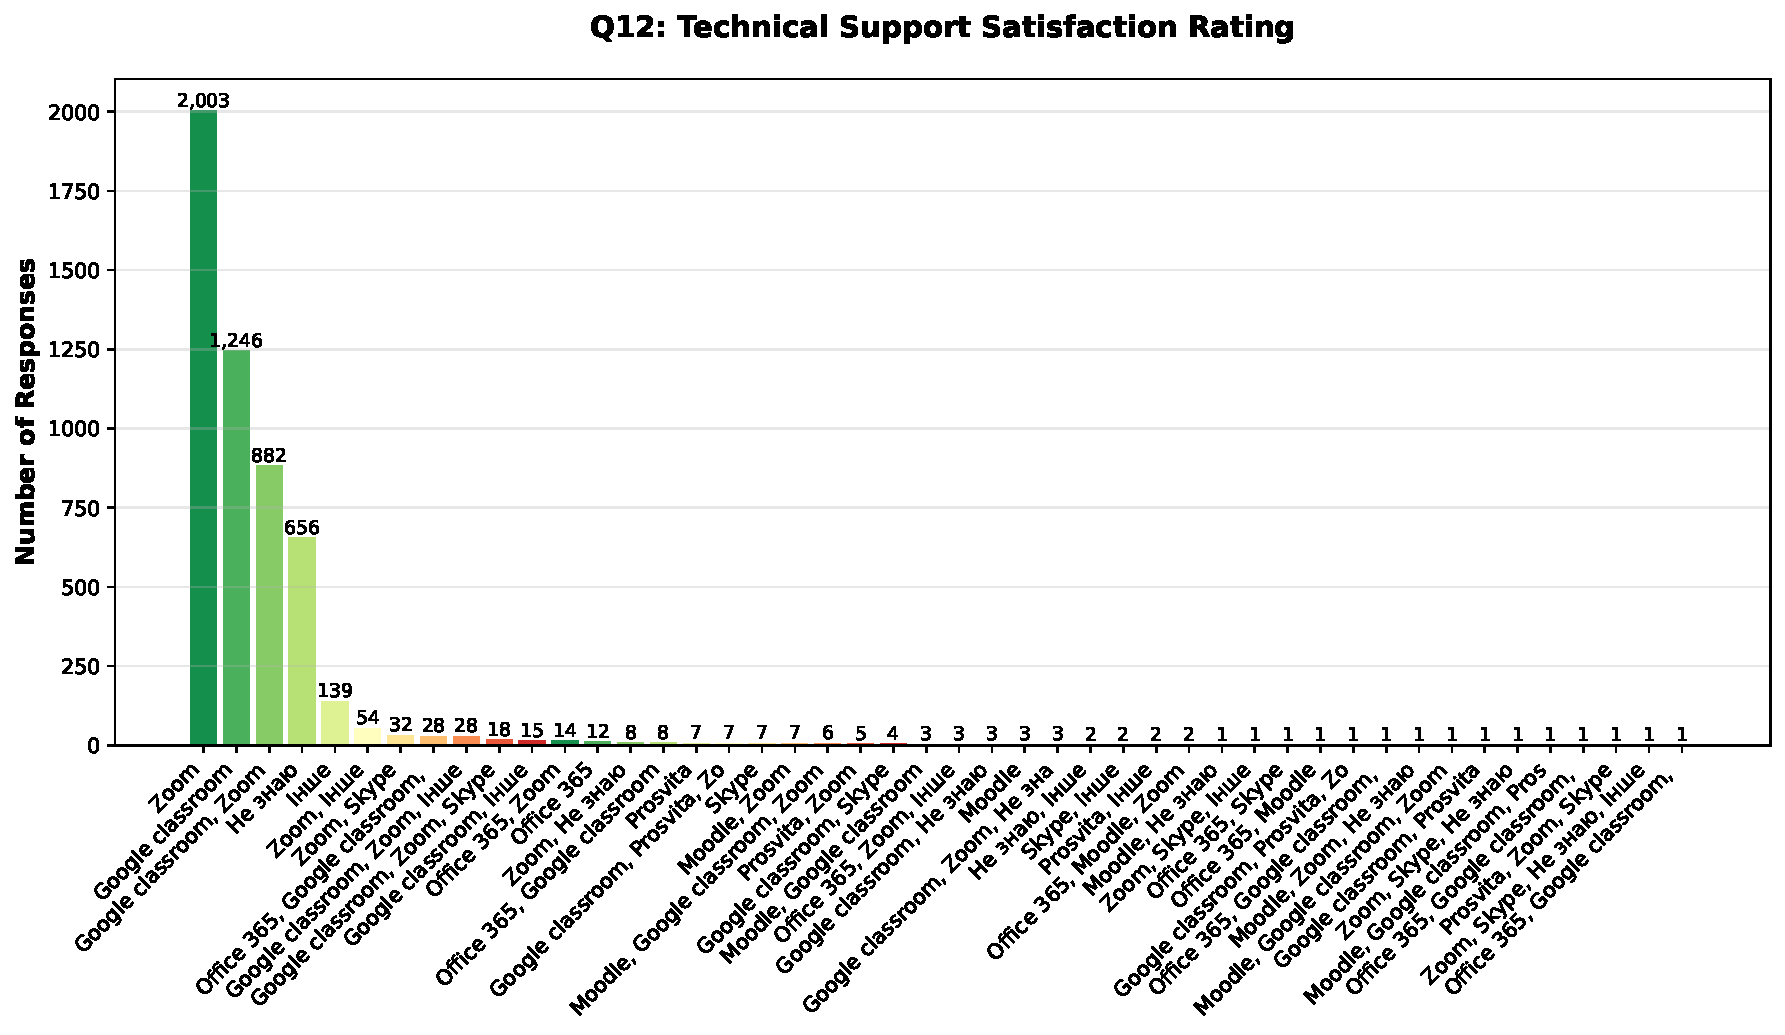
\includegraphics[width=\textwidth]{../visualizations/all_questions/q12_tech_support_satisfaction.pdf}
        \caption{Q12: Technical support satisfaction}
        \label{fig:q12_tech}
    \end{subfigure}
    \hfill
    \begin{subfigure}[b]{0.48\textwidth}
        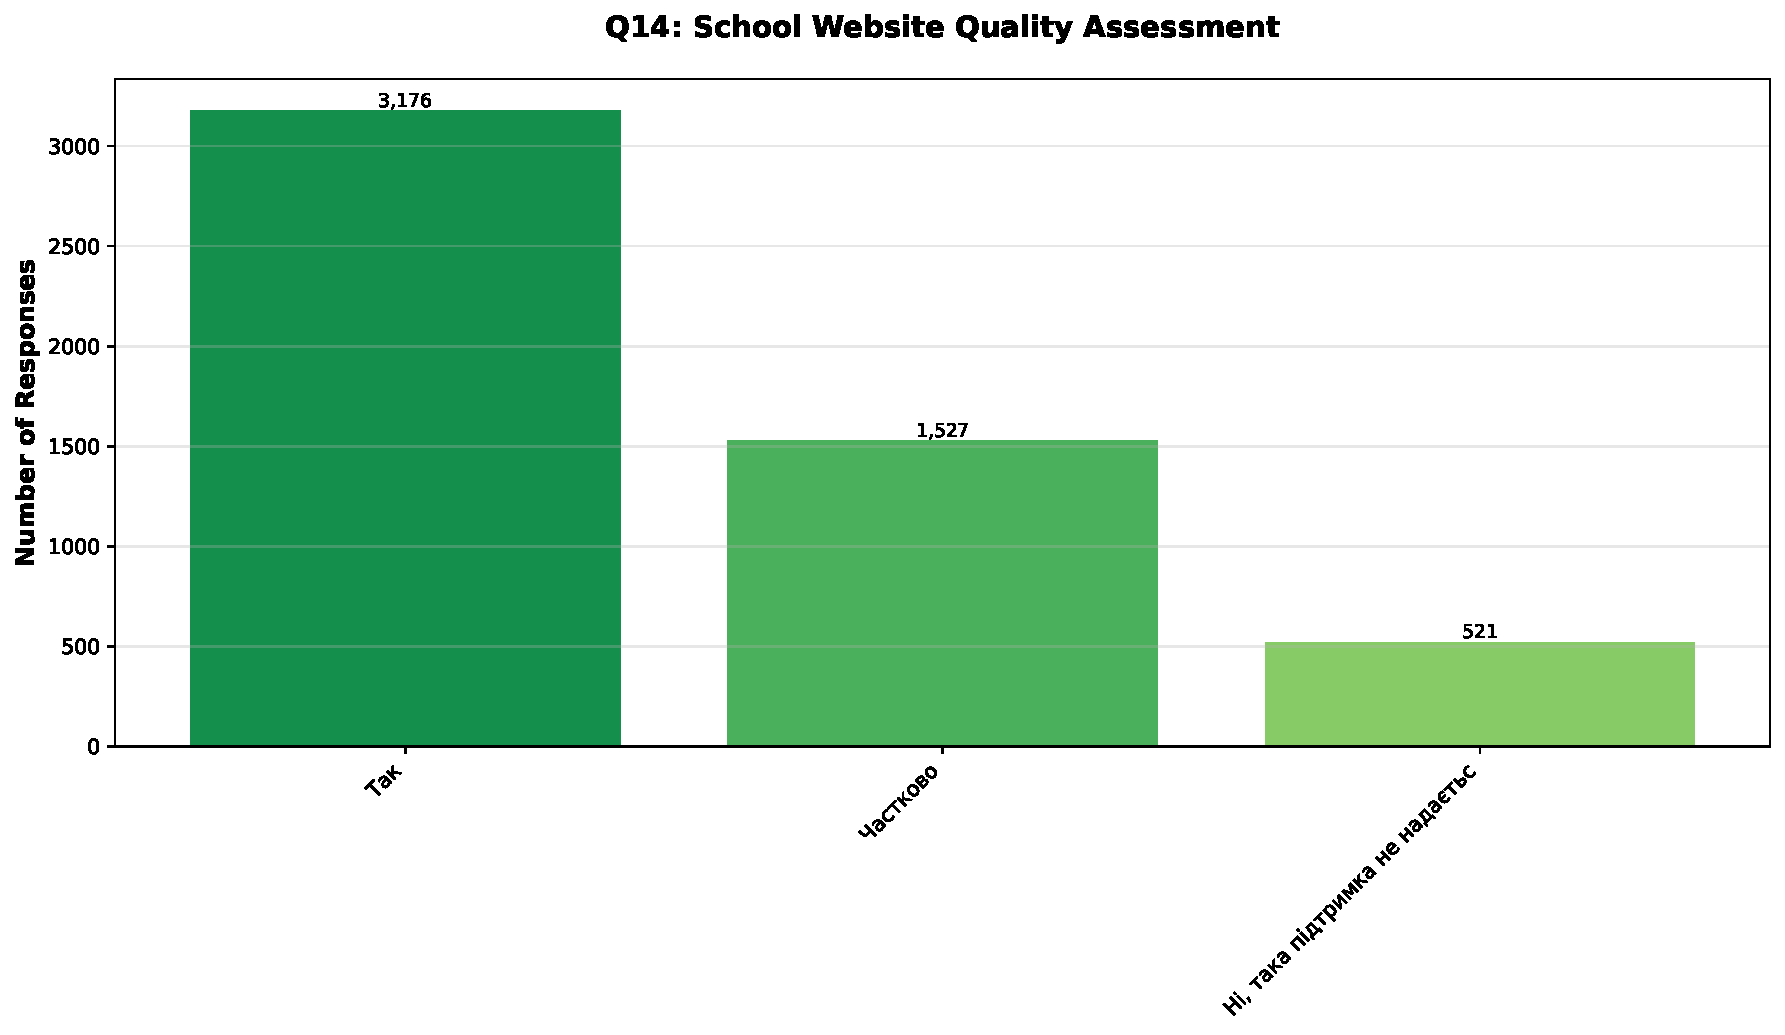
\includegraphics[width=\textwidth]{../visualizations/all_questions/q14_website_quality.pdf}
        \caption{Q14: School website quality}
        \label{fig:q14_website}
    \end{subfigure}
    \caption{Technical Support and Website Quality - Parent satisfaction ratings for school digital services.}
    \label{fig:satisfaction_tech}
\end{figure}

\begin{figure}[H]
    \centering
    \begin{subfigure}[b]{0.48\textwidth}
        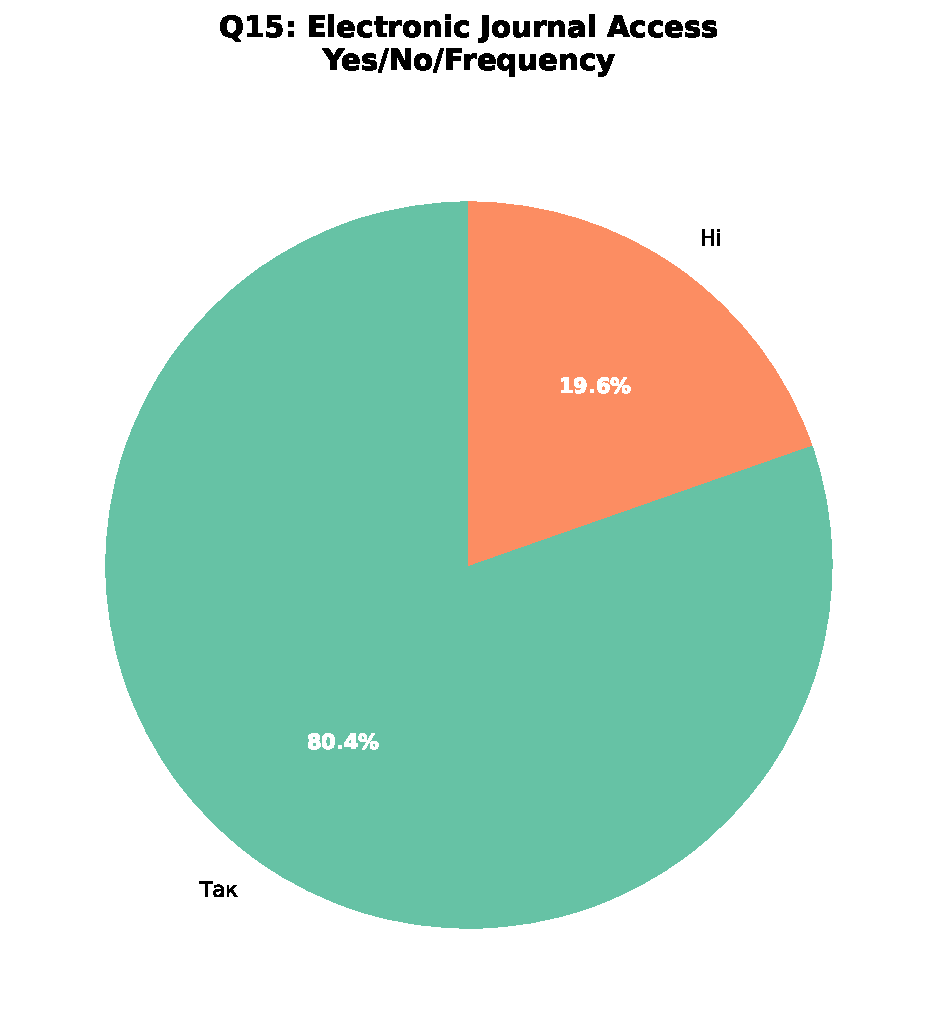
\includegraphics[width=\textwidth]{../visualizations/all_questions/q15_journal_access.pdf}
        \caption{Q15: Electronic journal access}
        \label{fig:q15_journal}
    \end{subfigure}
    \hfill
    \begin{subfigure}[b]{0.48\textwidth}
        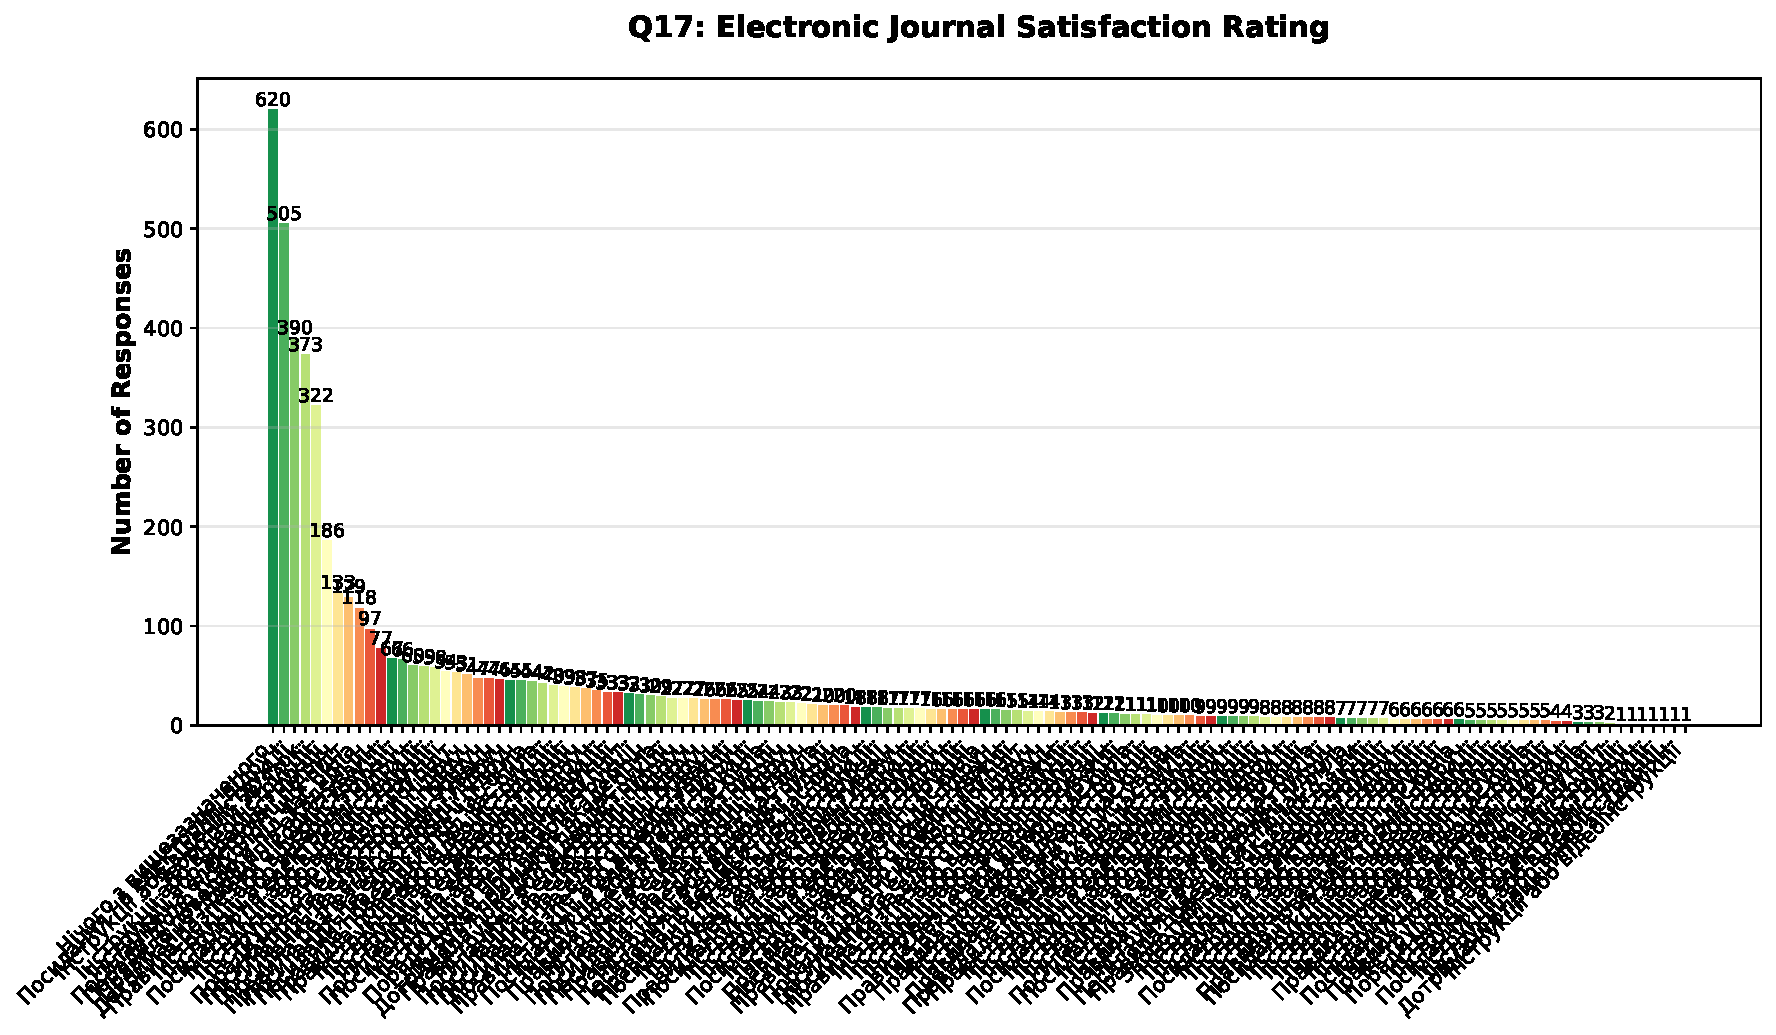
\includegraphics[width=\textwidth]{../visualizations/all_questions/q17_journal_satisfaction.pdf}
        \caption{Q17: Electronic journal satisfaction}
        \label{fig:q17_journal_sat}
    \end{subfigure}
    \caption{Electronic Journal Access and Satisfaction - Availability and quality ratings for digital grade books and student information systems.}
    \label{fig:journal}
\end{figure}

\newpage

%===================================================================================
\section{Competencies \& Engagement (Q18-Q21)}
%===================================================================================

\begin{figure}[H]
    \centering
    \begin{subfigure}[b]{0.48\textwidth}
        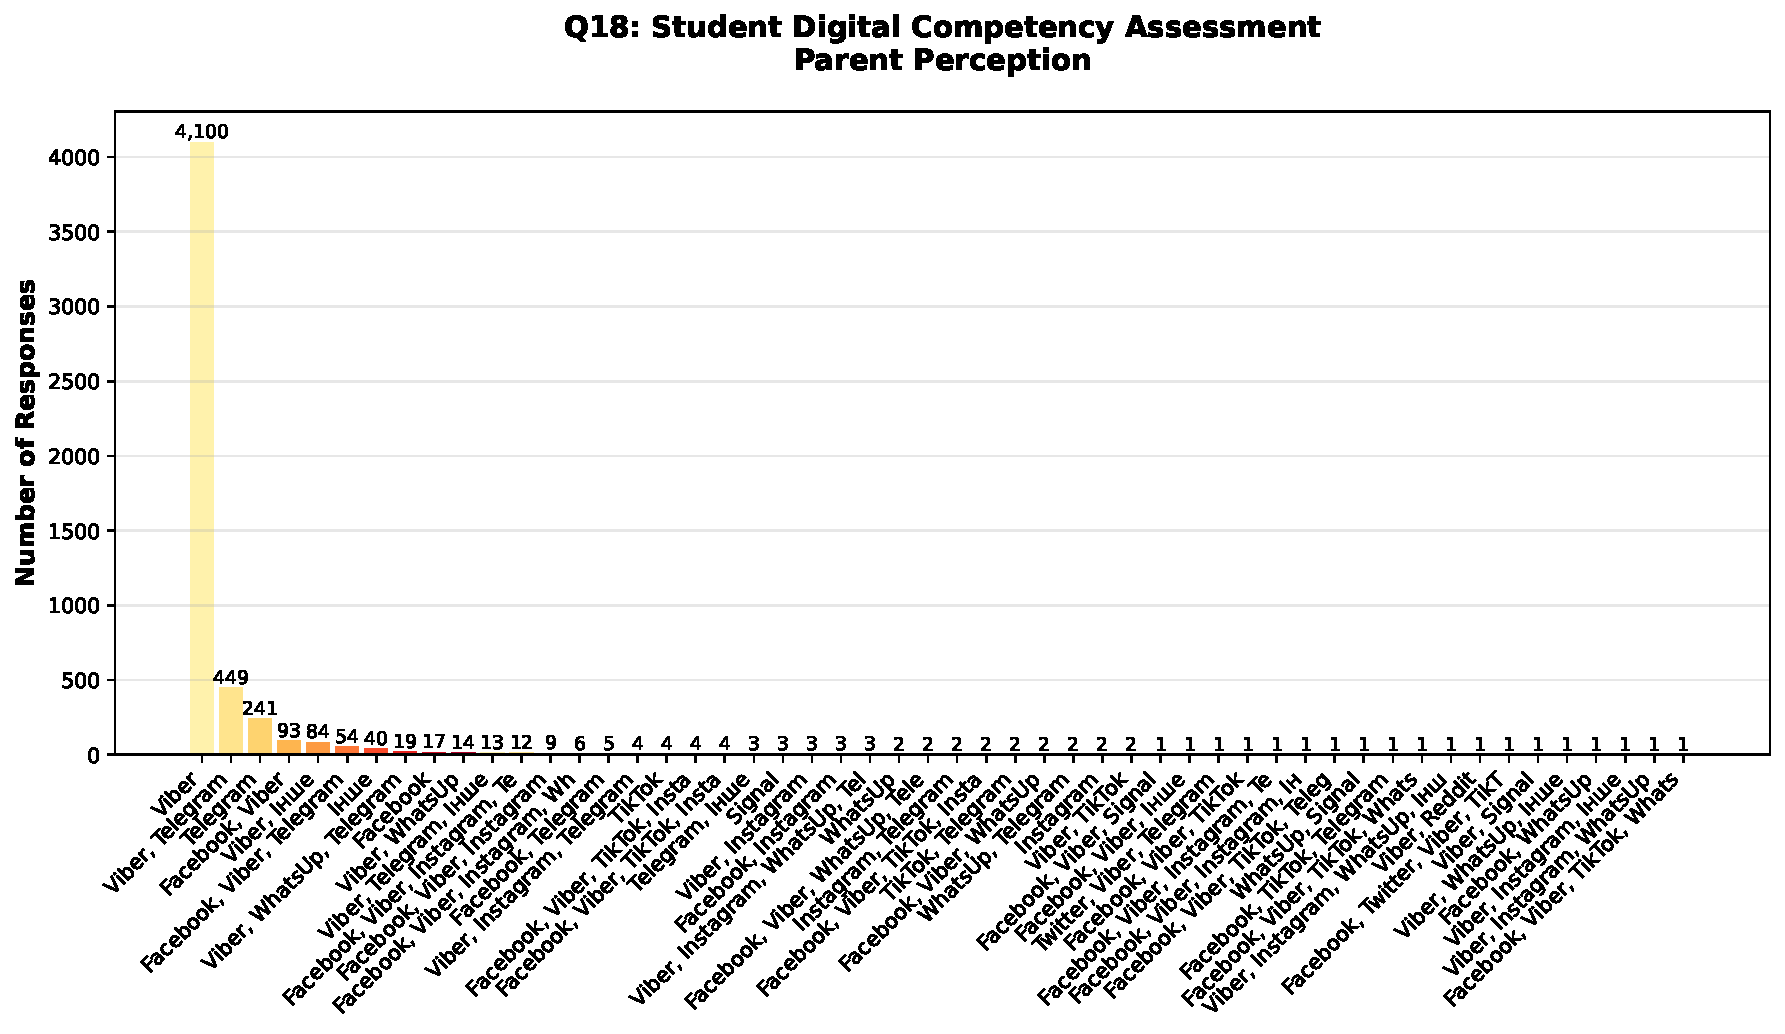
\includegraphics[width=\textwidth]{../visualizations/all_questions/q18_digital_skills.pdf}
        \caption{Q18: Student digital competency (parent assessment)}
        \label{fig:q18_skills}
    \end{subfigure}
    \hfill
    \begin{subfigure}[b]{0.48\textwidth}
        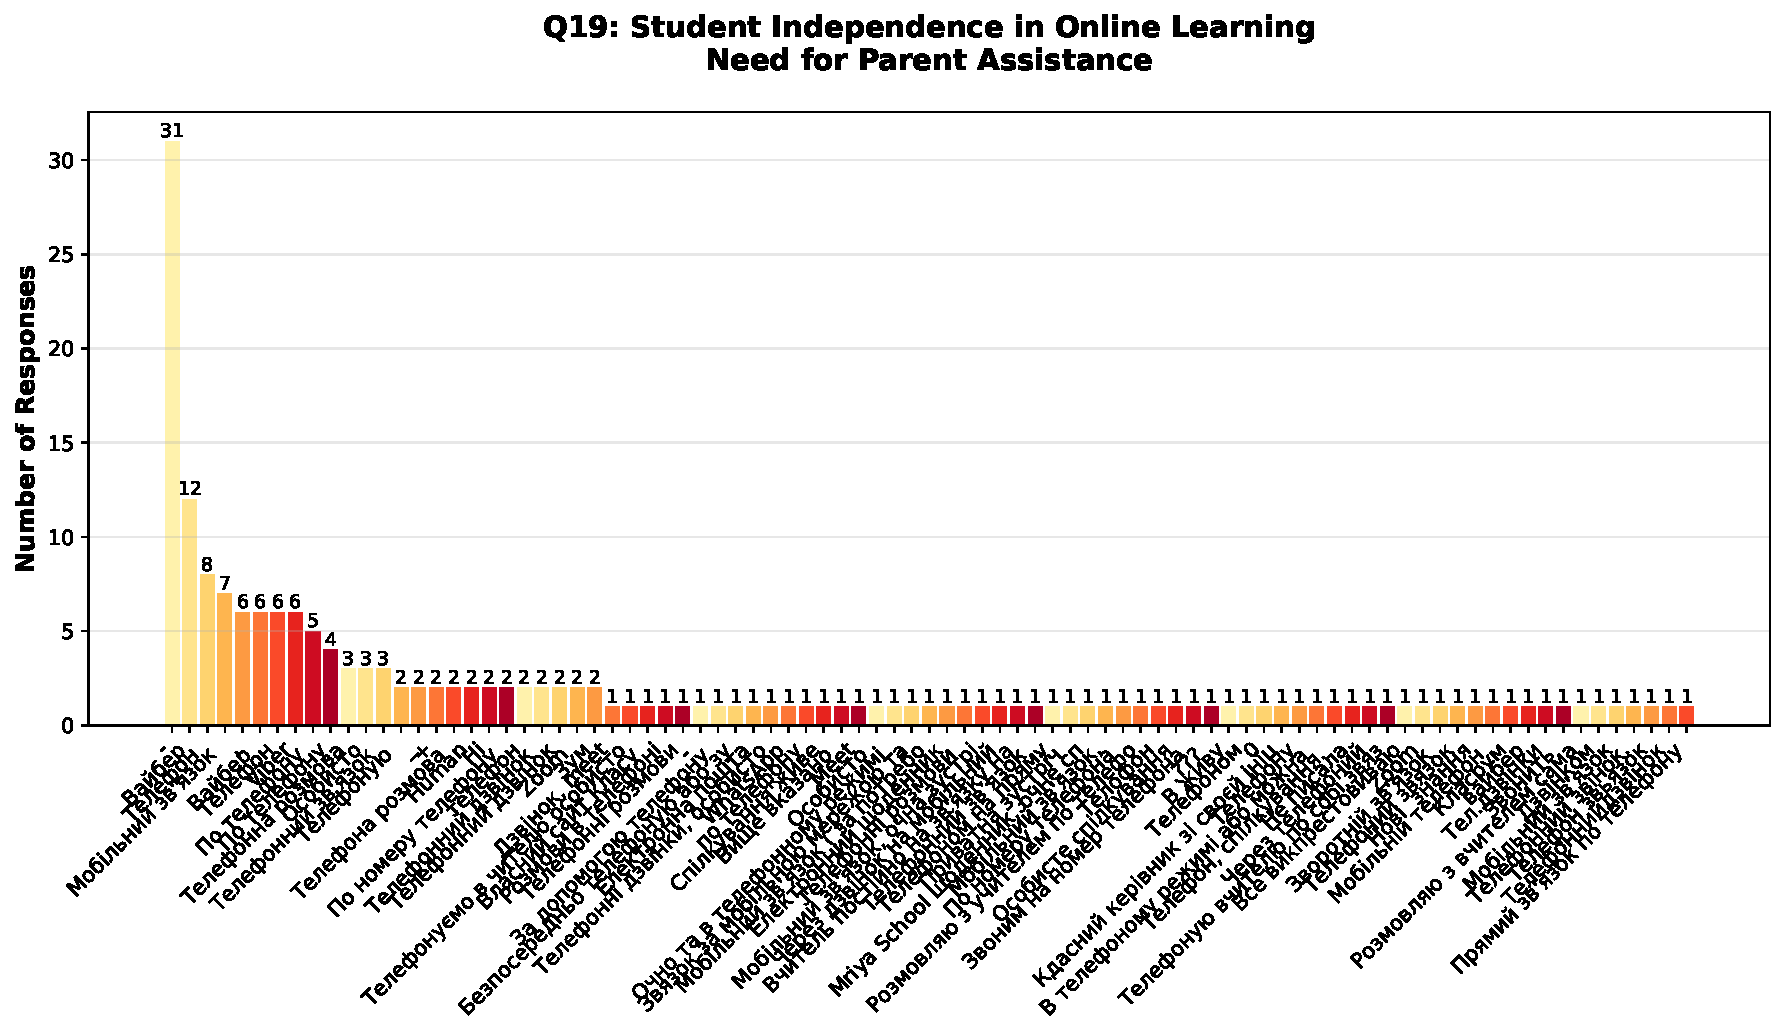
\includegraphics[width=\textwidth]{../visualizations/all_questions/q19_student_independence.pdf}
        \caption{Q19: Student independence in online learning}
        \label{fig:q19_independence}
    \end{subfigure}
    \caption{Student Digital Competencies - Parent perceptions of student digital skills and independence in online learning environments.}
    \label{fig:competencies}
\end{figure}

\begin{figure}[H]
    \centering
    \begin{subfigure}[b]{0.48\textwidth}
        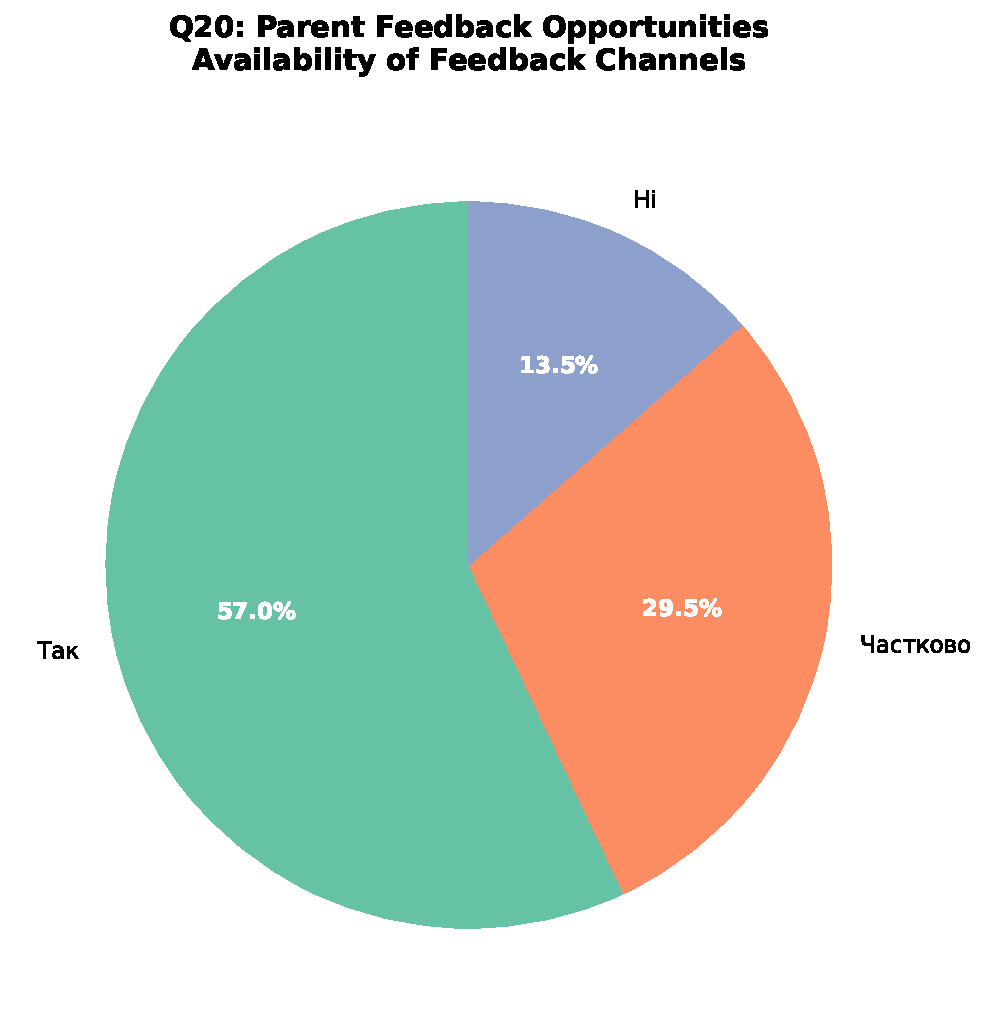
\includegraphics[width=\textwidth]{../visualizations/all_questions/q20_feedback_opportunities.pdf}
        \caption{Q20: Parent feedback opportunities}
        \label{fig:q20_feedback}
    \end{subfigure}
    \hfill
    \begin{subfigure}[b]{0.48\textwidth}
        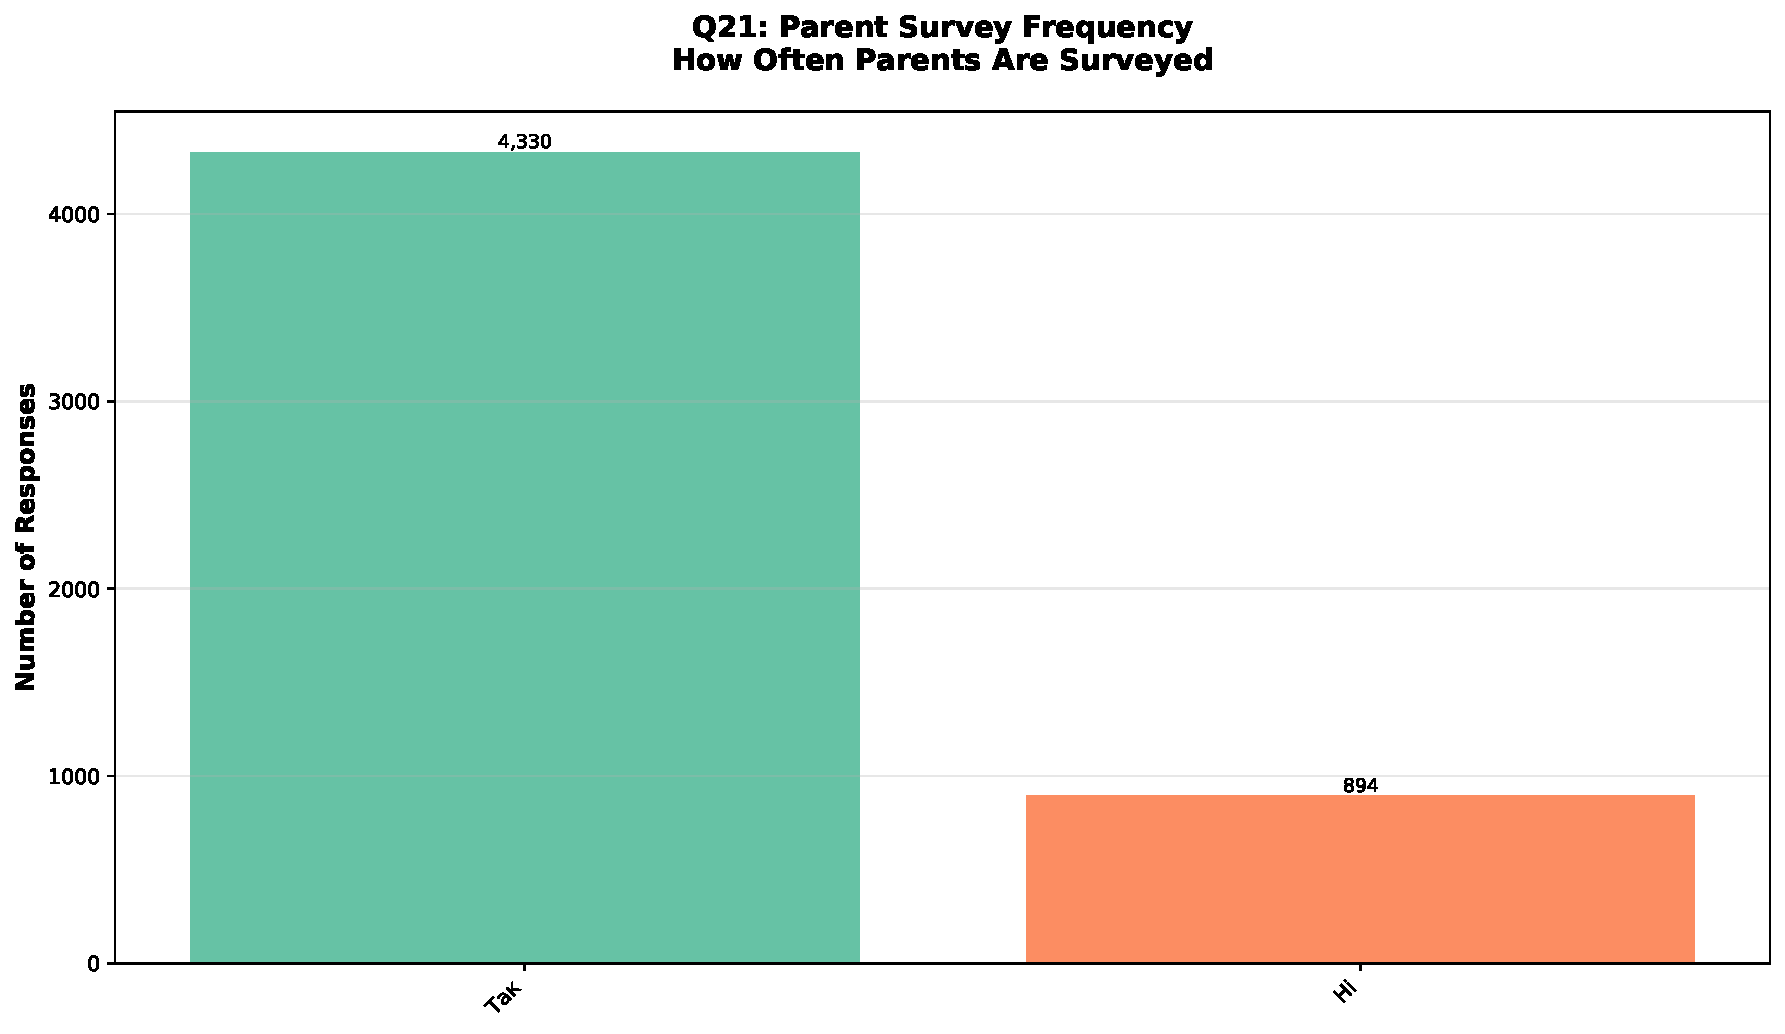
\includegraphics[width=\textwidth]{../visualizations/all_questions/q21_survey_frequency.pdf}
        \caption{Q21: Parent survey frequency}
        \label{fig:q21_surveys}
    \end{subfigure}
    \caption{Parent Engagement - Availability of feedback channels and frequency of parent surveys conducted by schools.}
    \label{fig:engagement}
\end{figure}

\newpage

%===================================================================================
\section{Q22: Parent Suggestions - Deep Analysis}
%===================================================================================

Question 22 asked parents: \textit{``What, in your opinion, could be improved in the digital information environment of your educational institution? (Please describe your suggestions)''} This open-ended question received 5,223 responses (99.98\% response rate) and was analyzed using advanced NLP methods.

\subsection{Response Quality and Sentiment}

\begin{figure}[H]
    \centering
    \begin{subfigure}[b]{0.48\textwidth}
        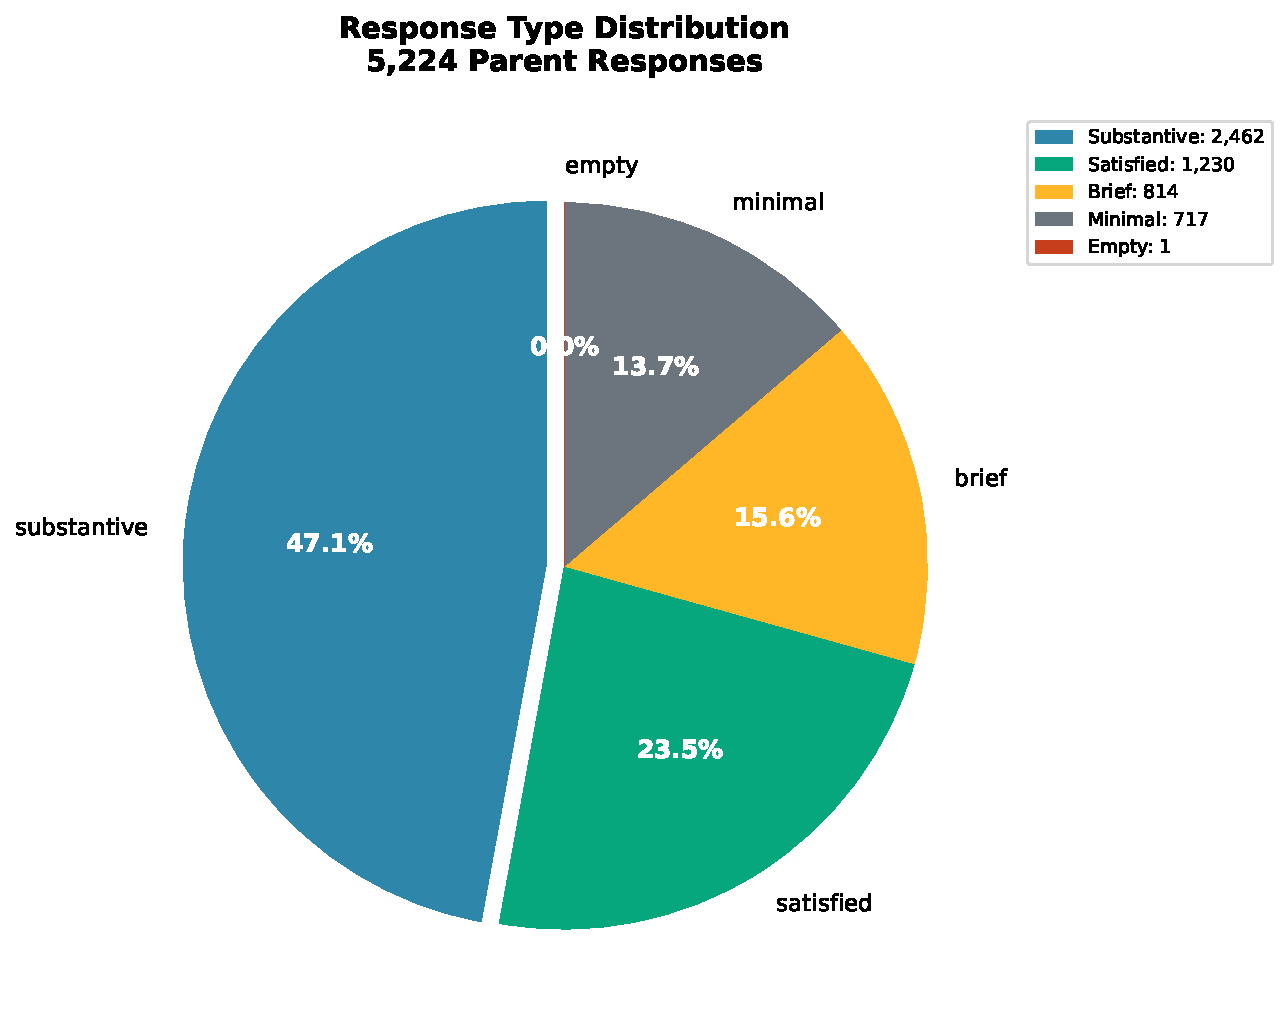
\includegraphics[width=\textwidth]{../visualizations/response_types.pdf}
        \caption{Response type classification}
        \label{fig:response_types}
    \end{subfigure}
    \hfill
    \begin{subfigure}[b]{0.48\textwidth}
        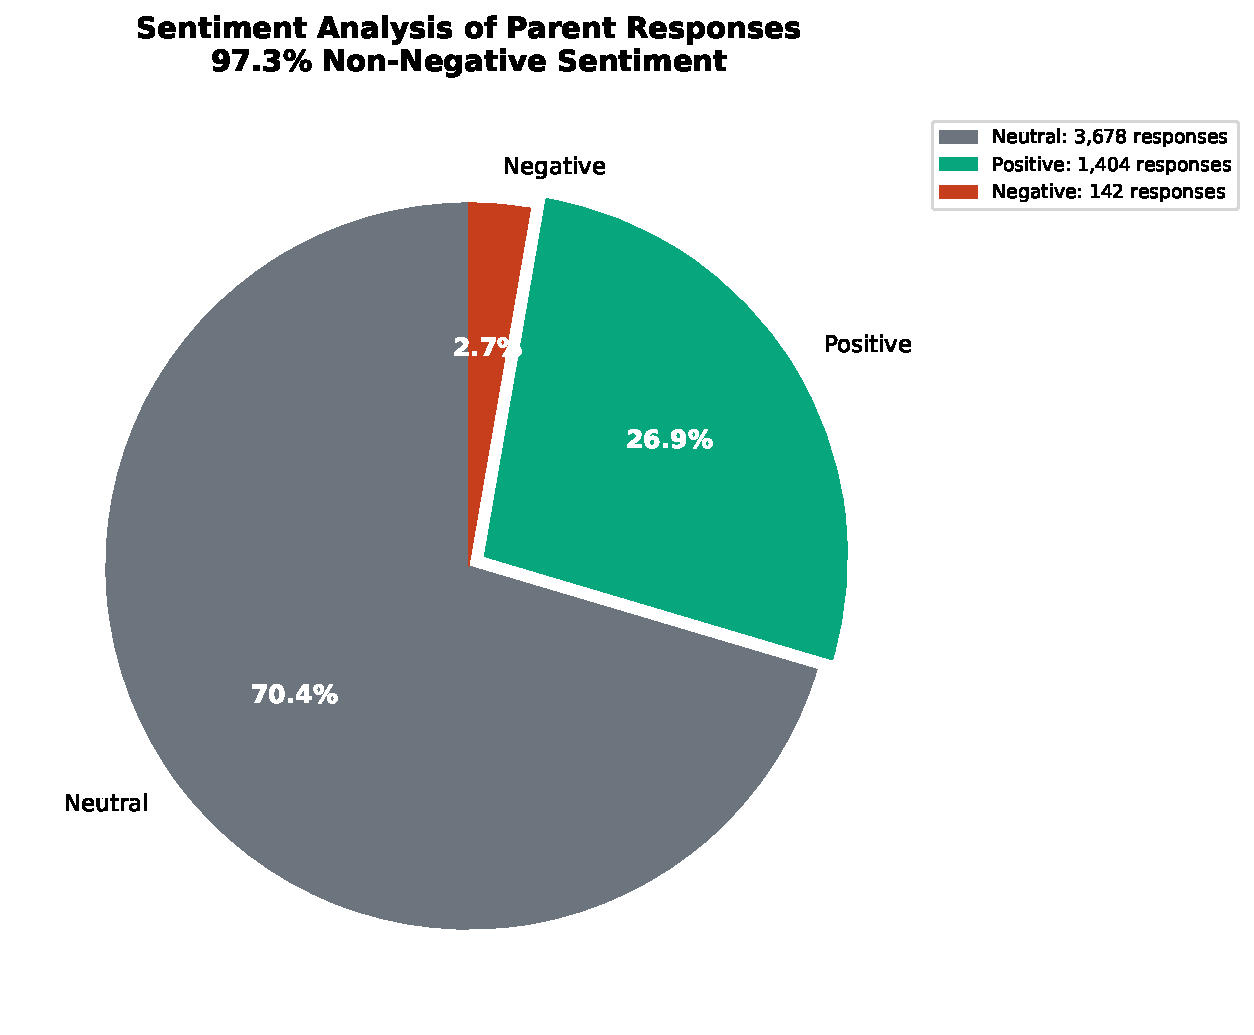
\includegraphics[width=\textwidth]{../visualizations/sentiment_distribution.pdf}
        \caption{Sentiment analysis: 97.3\% non-negative}
        \label{fig:sentiment}
    \end{subfigure}
    \caption{Q22 Response Quality - 47.1\% substantive suggestions and overwhelmingly constructive sentiment despite wartime challenges.}
    \label{fig:q22_quality}
\end{figure}

\begin{figure}[H]
    \centering
    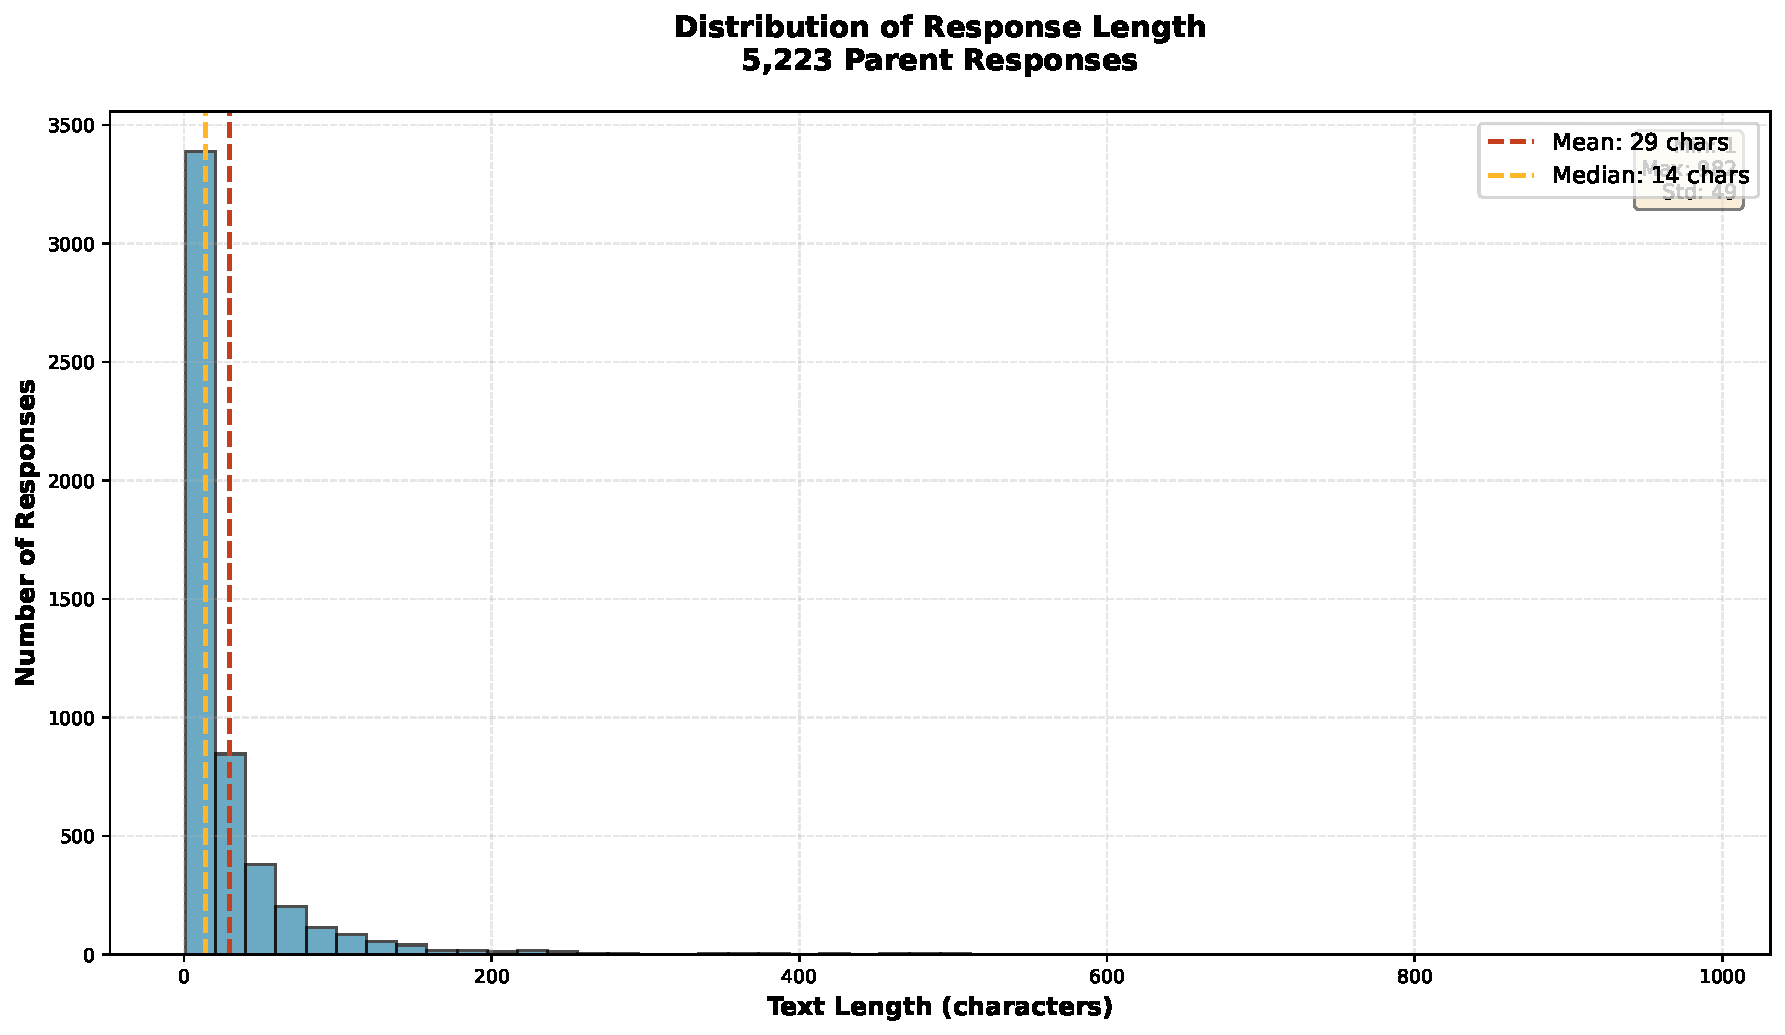
\includegraphics[width=0.9\textwidth]{../visualizations/text_length_distribution.pdf}
    \caption{Q22 Text Length Distribution - Mean: 29 characters, Median: 14 characters, Max: 982 characters. Distribution shows mix of brief acknowledgments and detailed suggestions.}
    \label{fig:text_length}
\end{figure}

\newpage

\subsection{Theme Distribution and Priorities}

\begin{figure}[H]
    \centering
    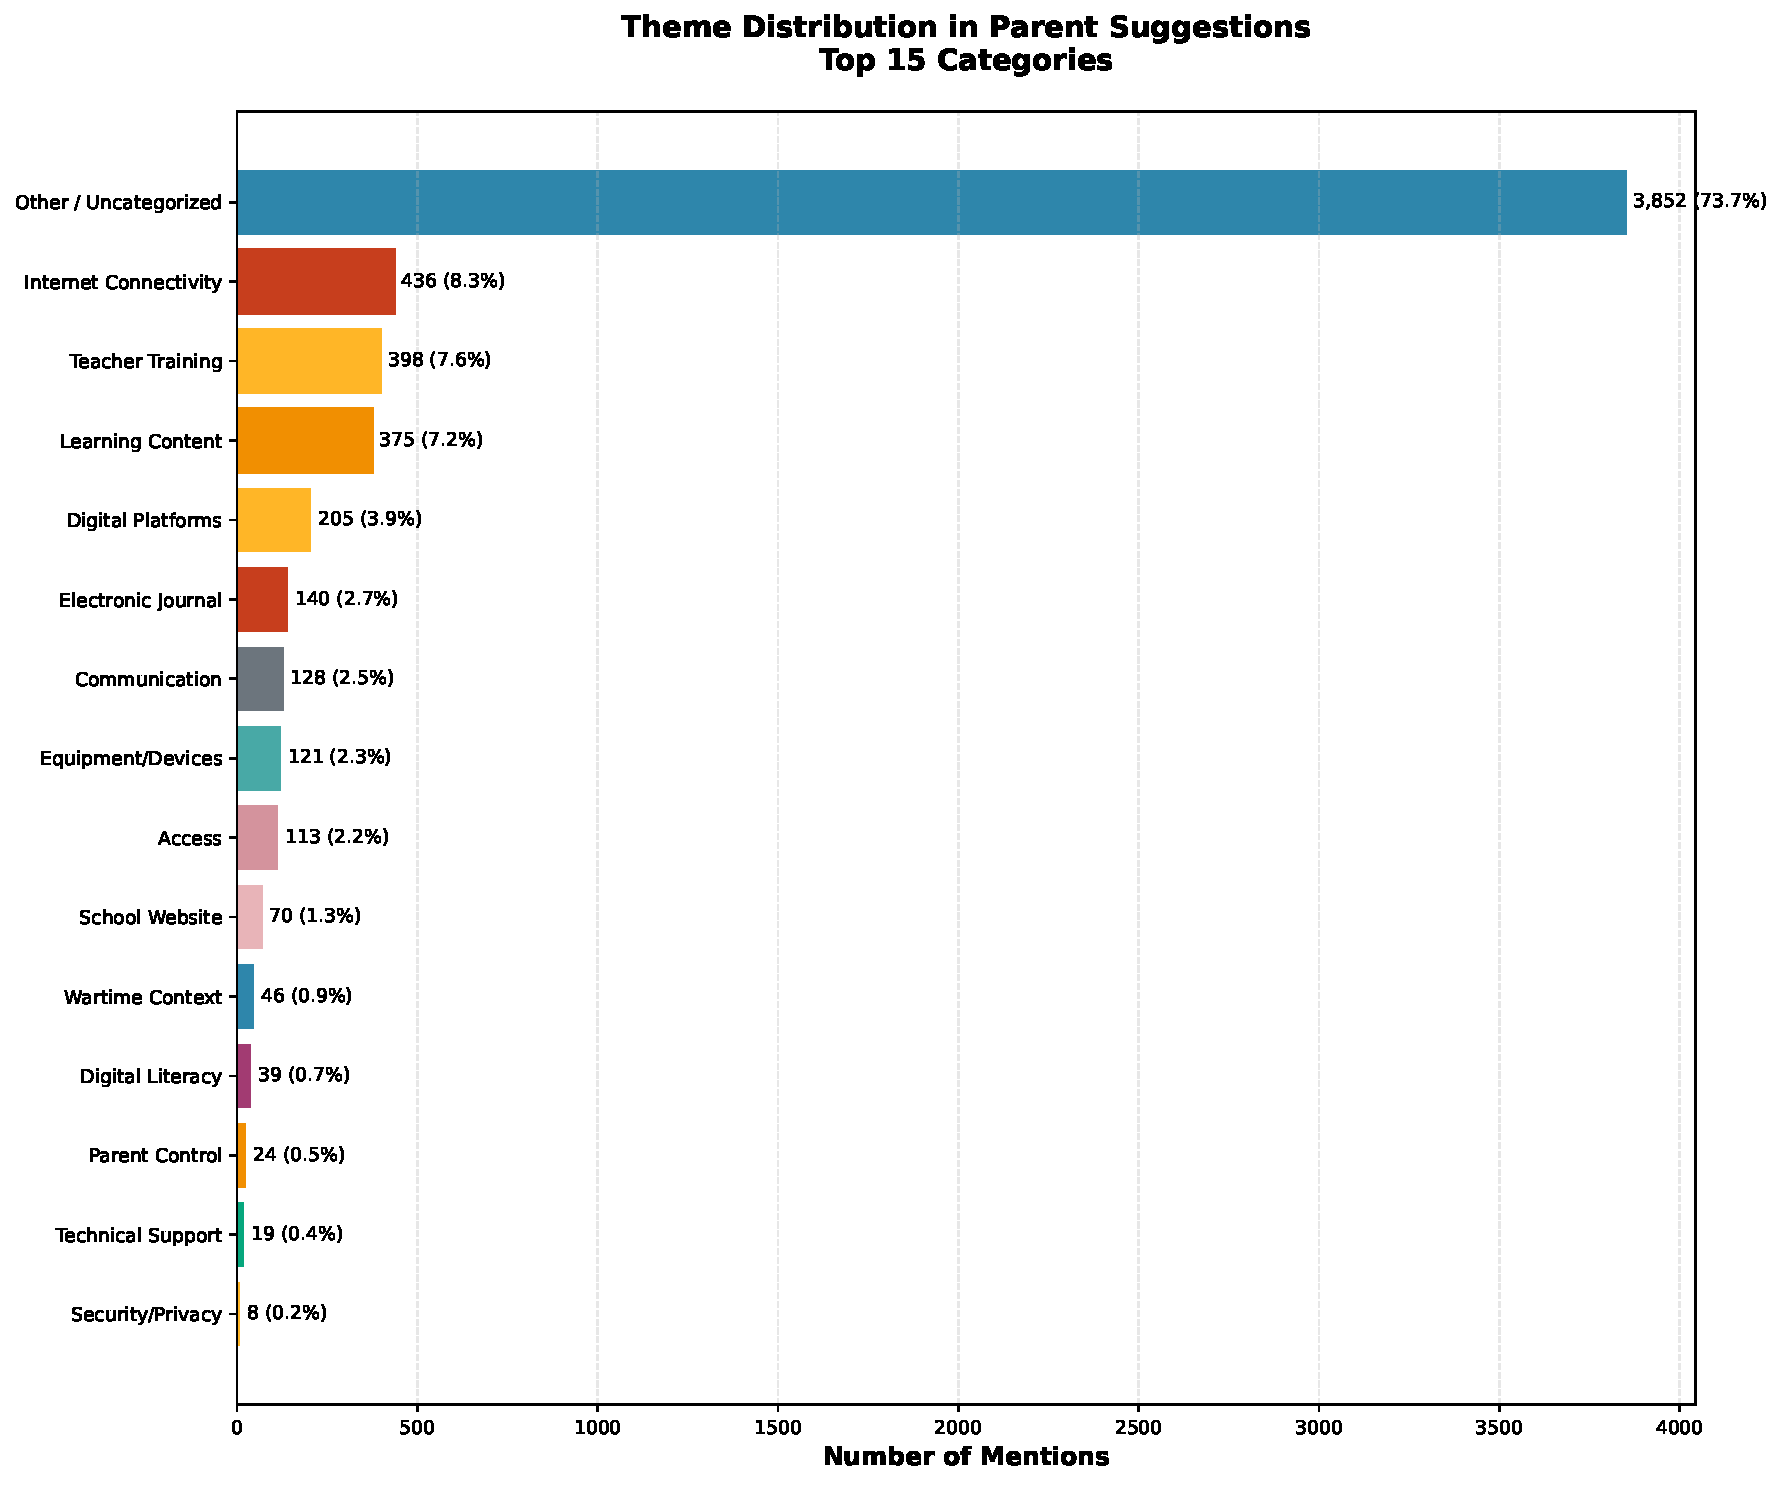
\includegraphics[width=\textwidth,height=0.95\textheight,keepaspectratio]{../visualizations/theme_distribution.pdf}
    \caption{Q22 Theme Distribution (Top 15) - Internet connectivity, teacher training, and learning content emerge as top 3 priorities. ``Other/Uncategorized'' represents satisfied parents or unique suggestions.}
    \label{fig:themes}
\end{figure}

\newpage

\subsection{Word Frequency Analysis}

\begin{figure}[H]
    \centering
    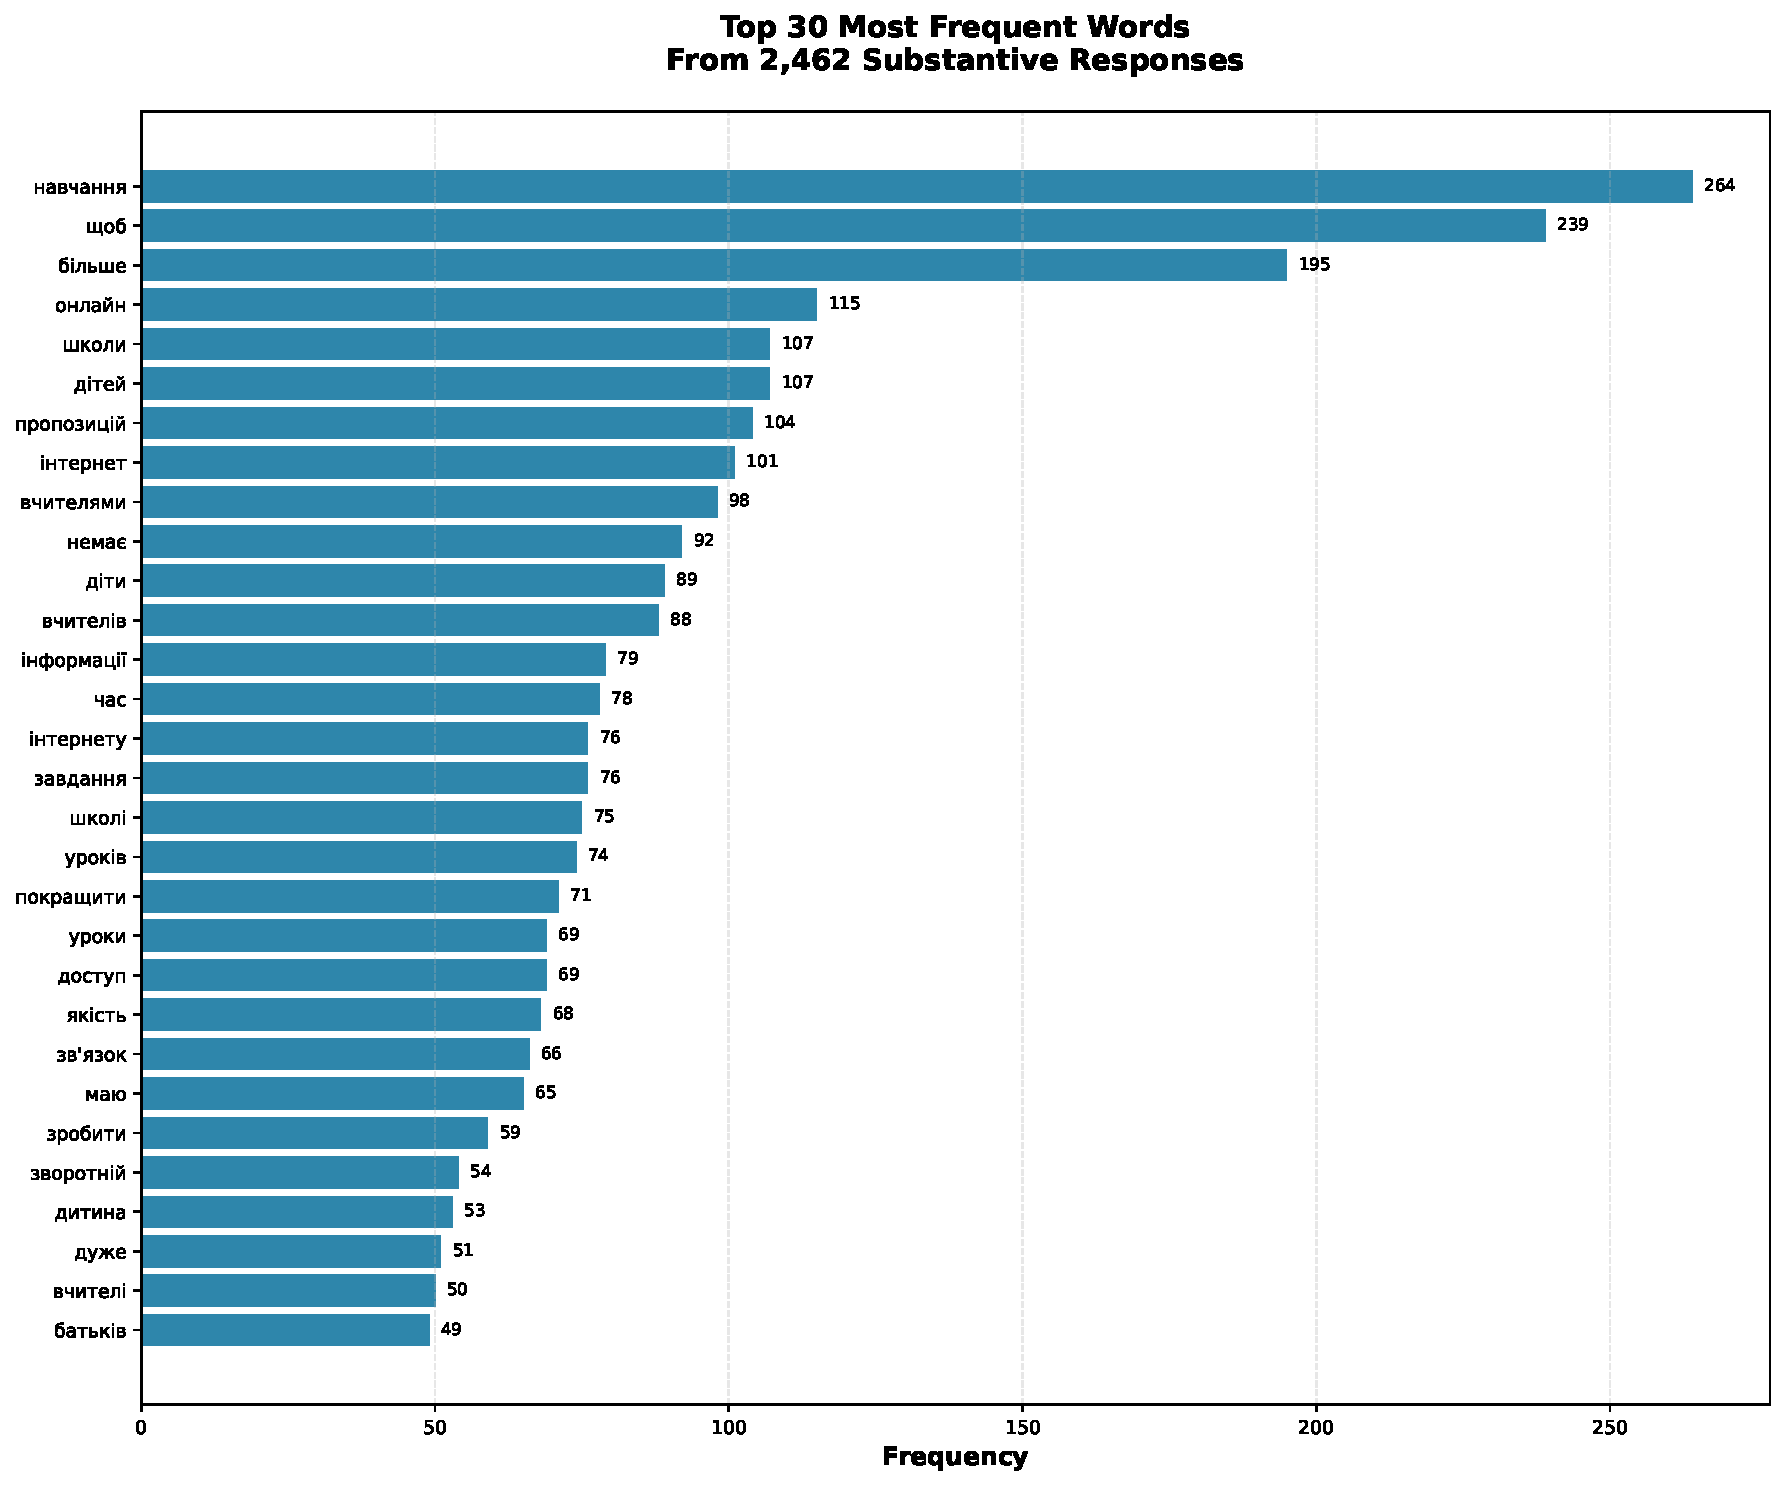
\includegraphics[width=\textwidth,height=0.9\textheight,keepaspectratio]{../visualizations/top_words.pdf}
    \caption{Q22 Top 30 Most Frequent Words - From 2,462 substantive responses after removing stopwords. ``Навчання'' (learning), ``щоб'' (so that/in order to), ``більше'' (more) dominate.}
    \label{fig:top_words}
\end{figure}

\begin{figure}[H]
    \centering
    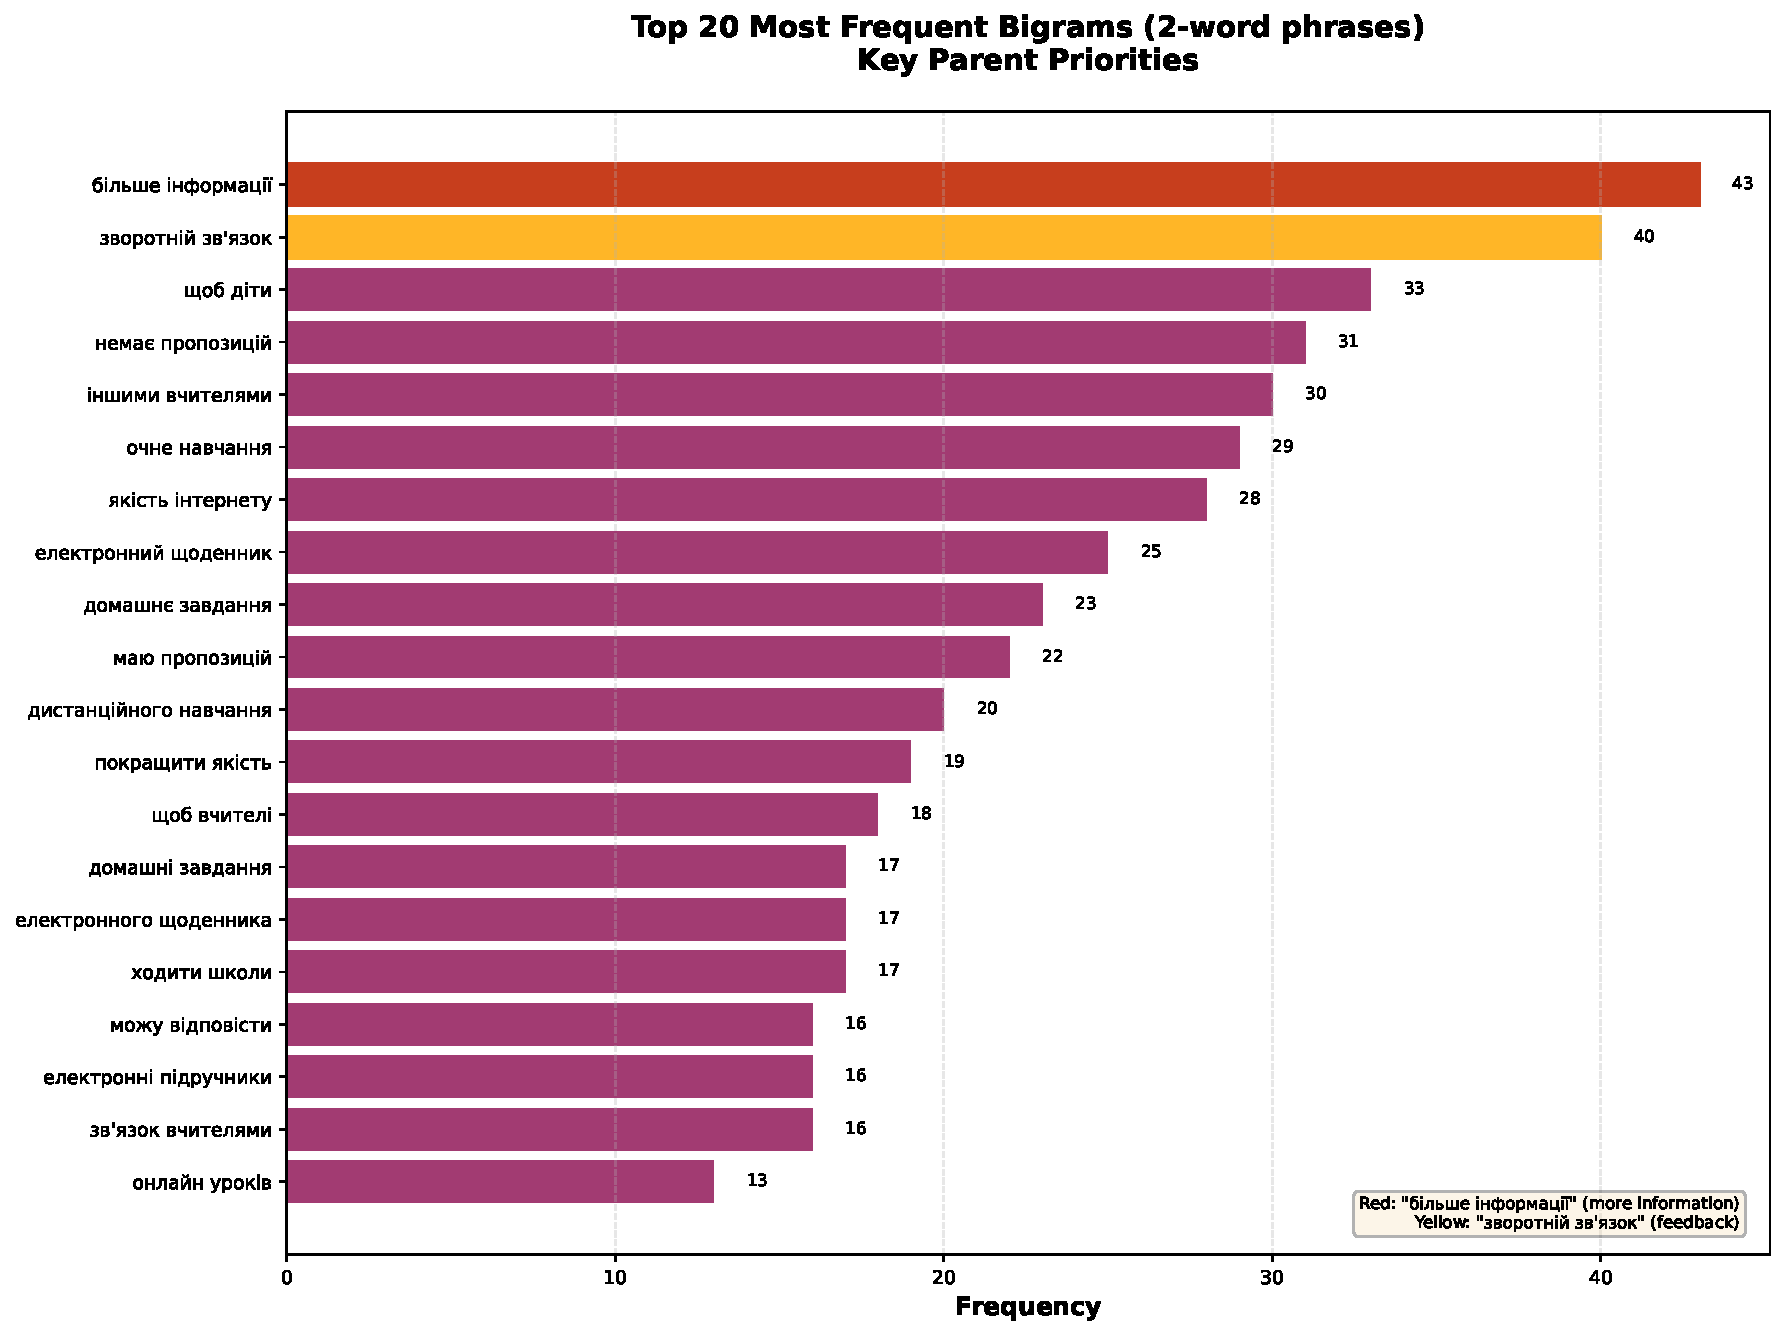
\includegraphics[width=\textwidth,height=0.85\textheight,keepaspectratio]{../visualizations/top_bigrams.pdf}
    \caption{Q22 Top 20 Bigrams (2-word phrases) - ``Більше інформації'' (more information) and ``зворотній зв'язок'' (feedback) are top parent requests, highlighting communication gaps.}
    \label{fig:bigrams}
\end{figure}

\newpage

\subsection{Word Cloud Visualization}

\begin{figure}[H]
    \centering
    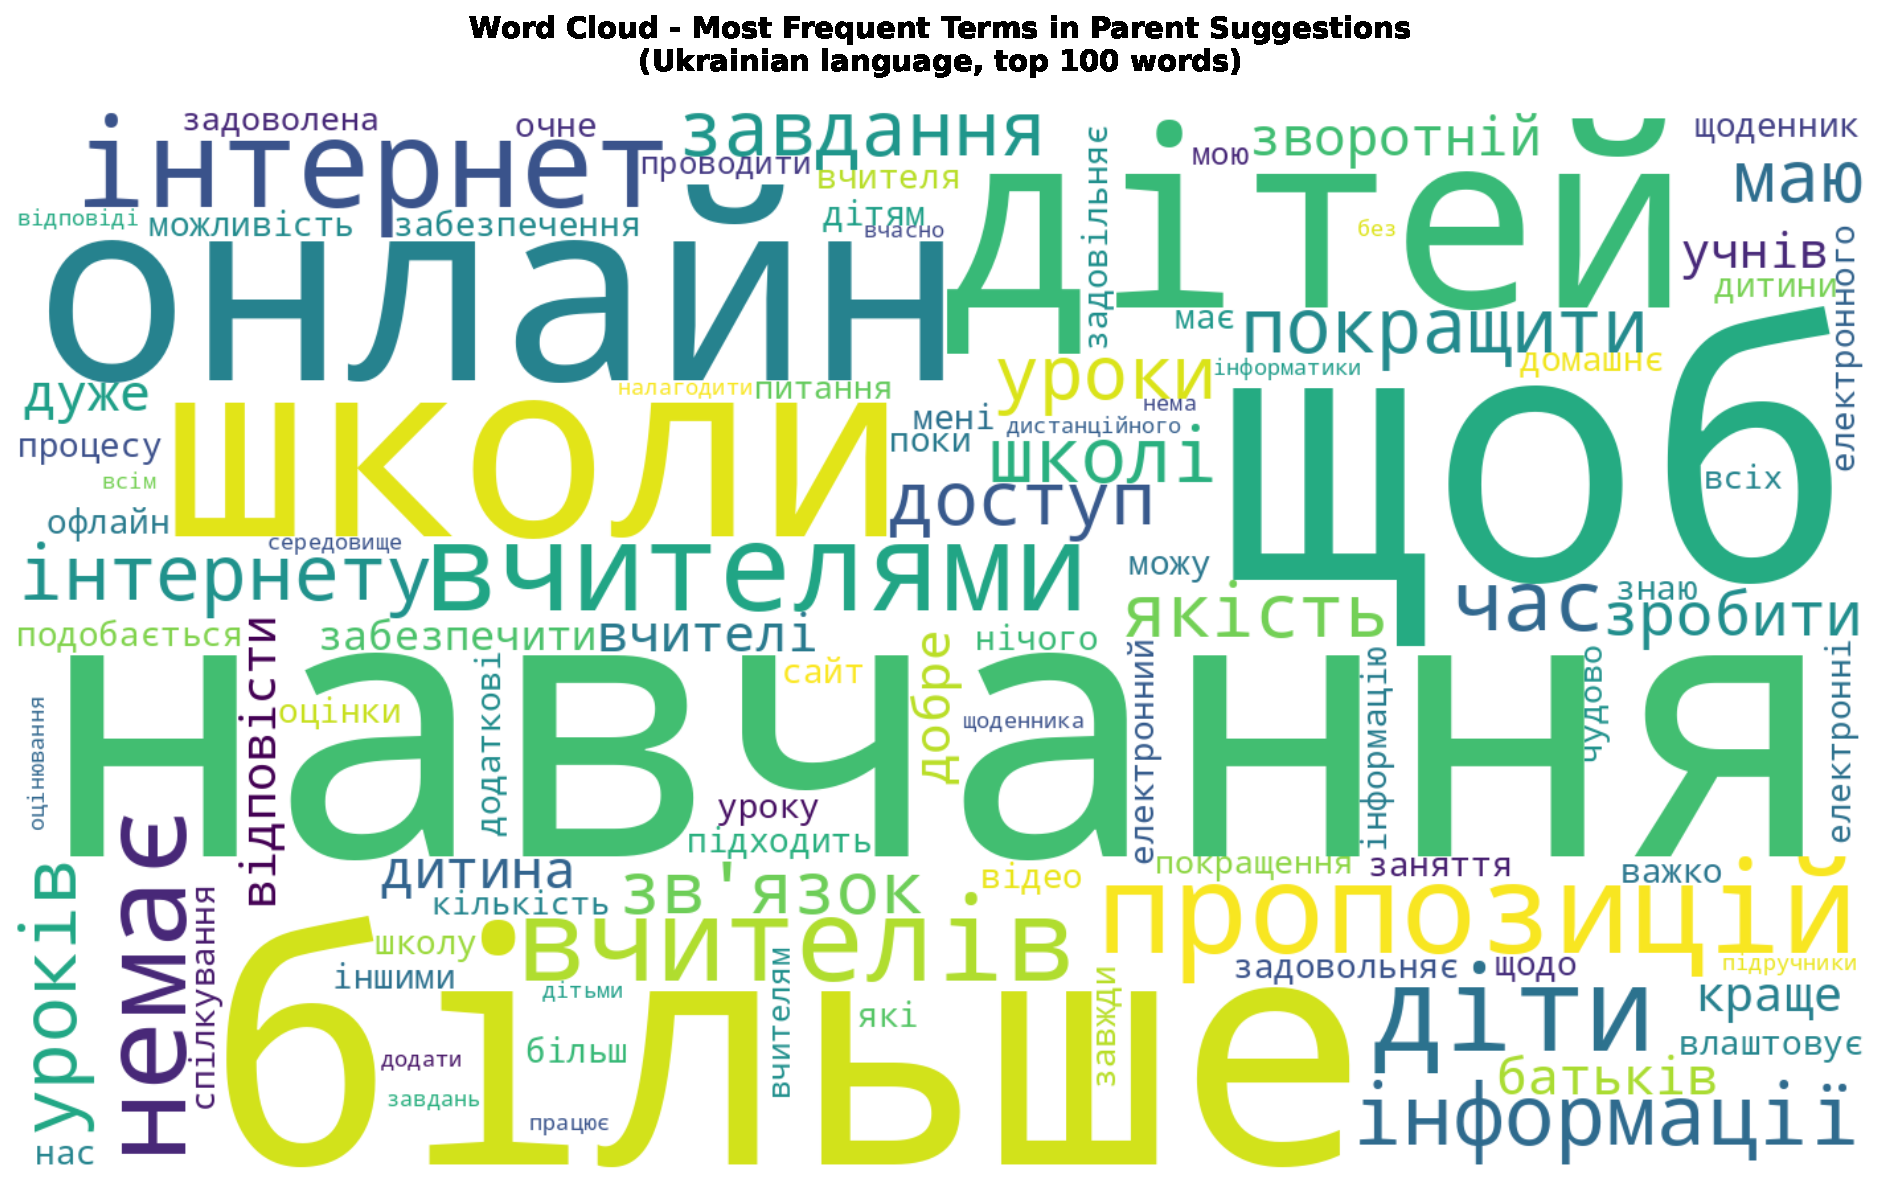
\includegraphics[width=\textwidth,height=0.85\textheight,keepaspectratio]{../visualizations/wordcloud.pdf}
    \caption{Q22 Word Cloud - Visual representation of top 100 words sized by frequency. Learning (навчання), more (більше), internet (інтернет), and teachers (вчителями) prominently featured.}
    \label{fig:wordcloud}
\end{figure}

\newpage

\subsection{Strategic Insights}

\begin{figure}[H]
    \centering
    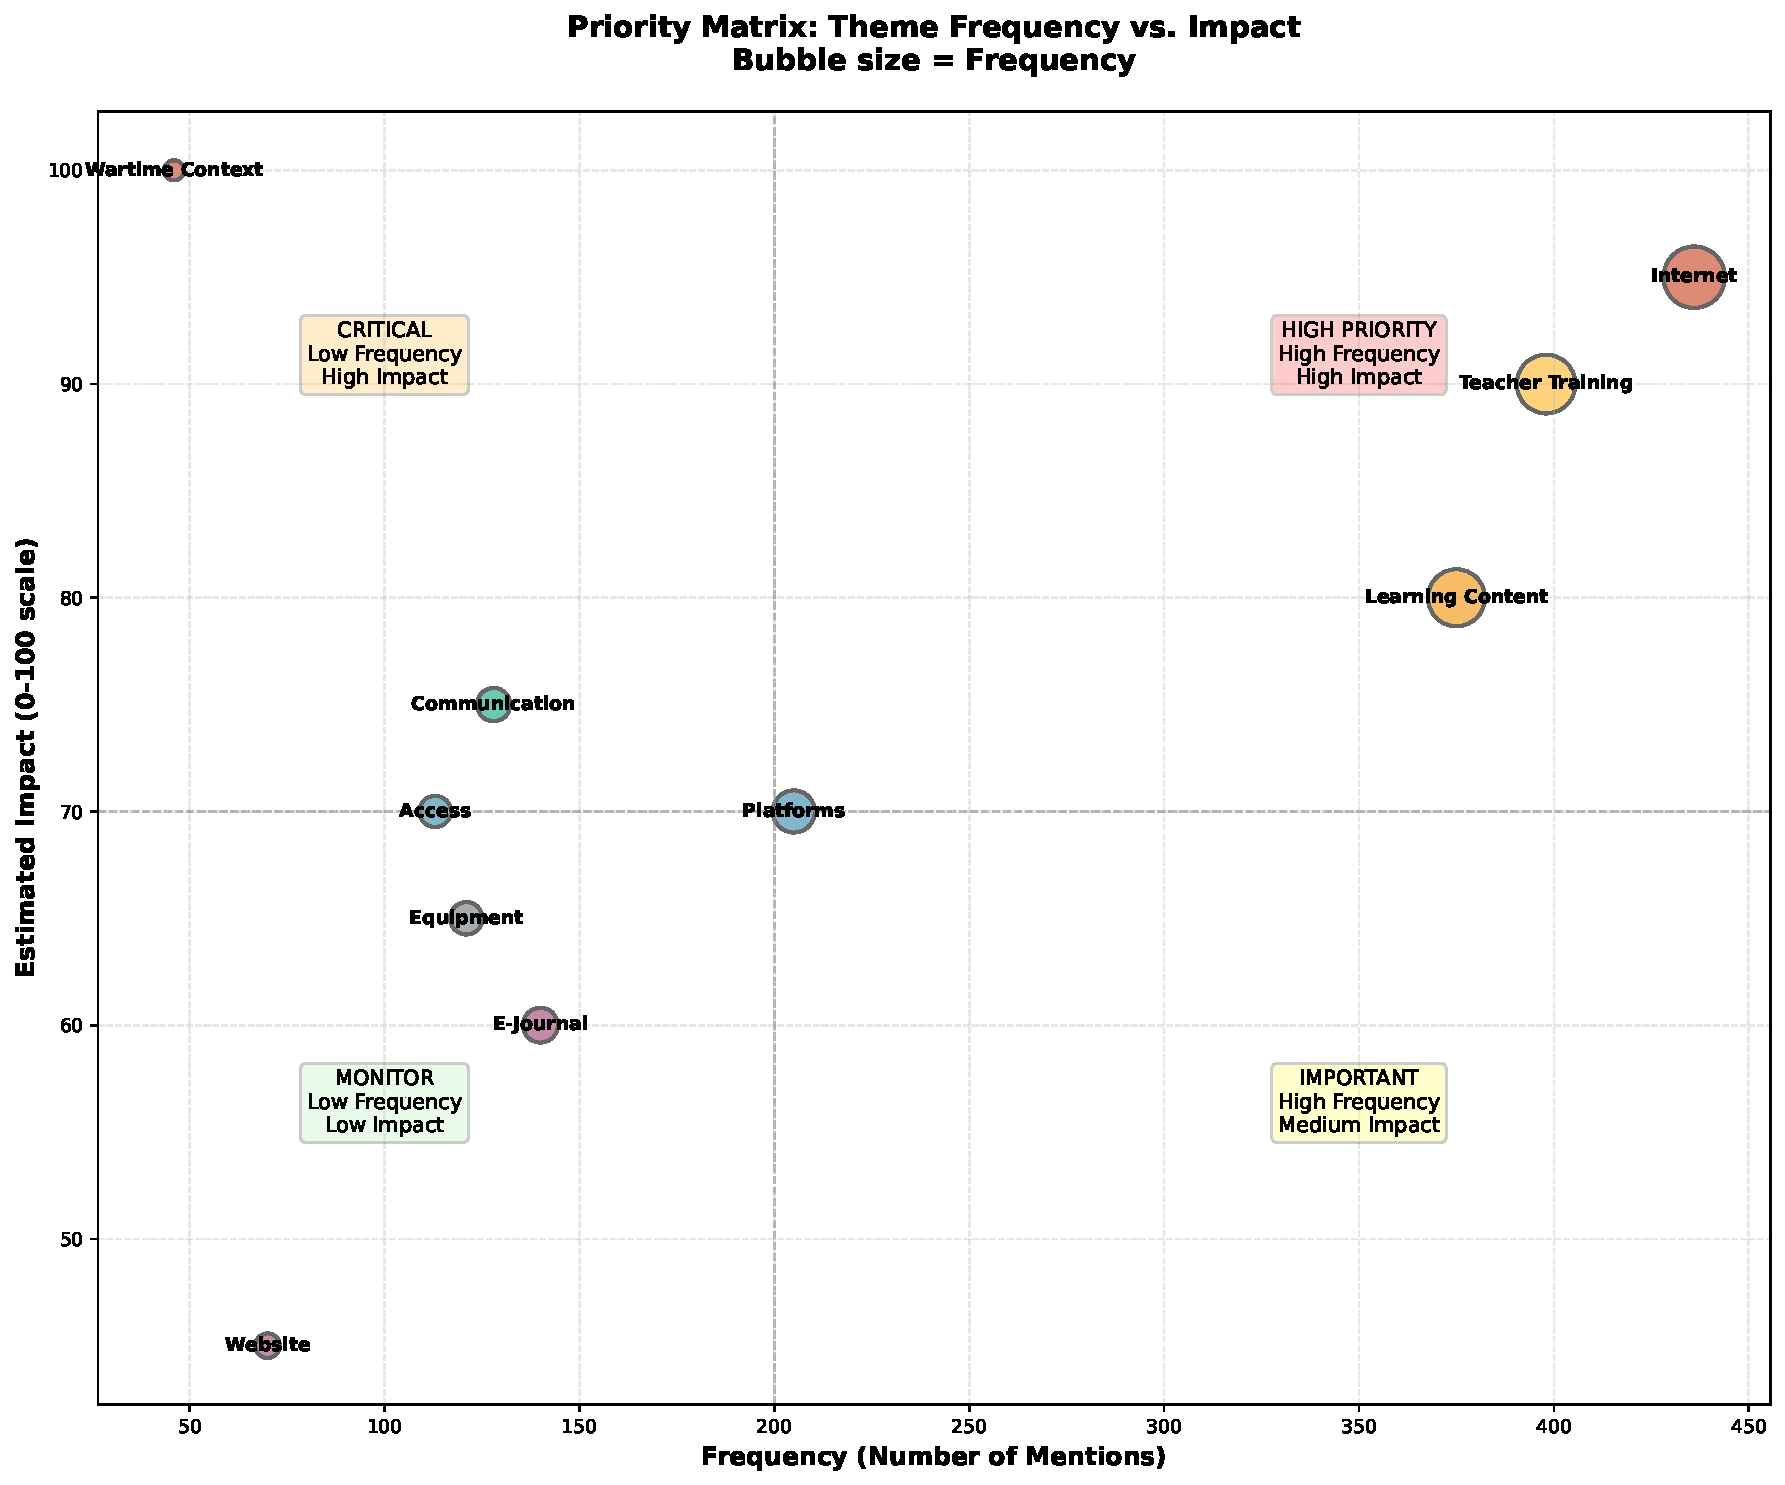
\includegraphics[width=\textwidth,height=0.85\textheight,keepaspectratio]{../visualizations/priority_matrix.pdf}
    \caption{Priority Matrix - Frequency vs. Impact - Bubble size indicates mention frequency. Internet, teacher training, and wartime context occupy high-priority quadrants requiring immediate policy attention.}
    \label{fig:priority_matrix}
\end{figure}

\begin{figure}[H]
    \centering
    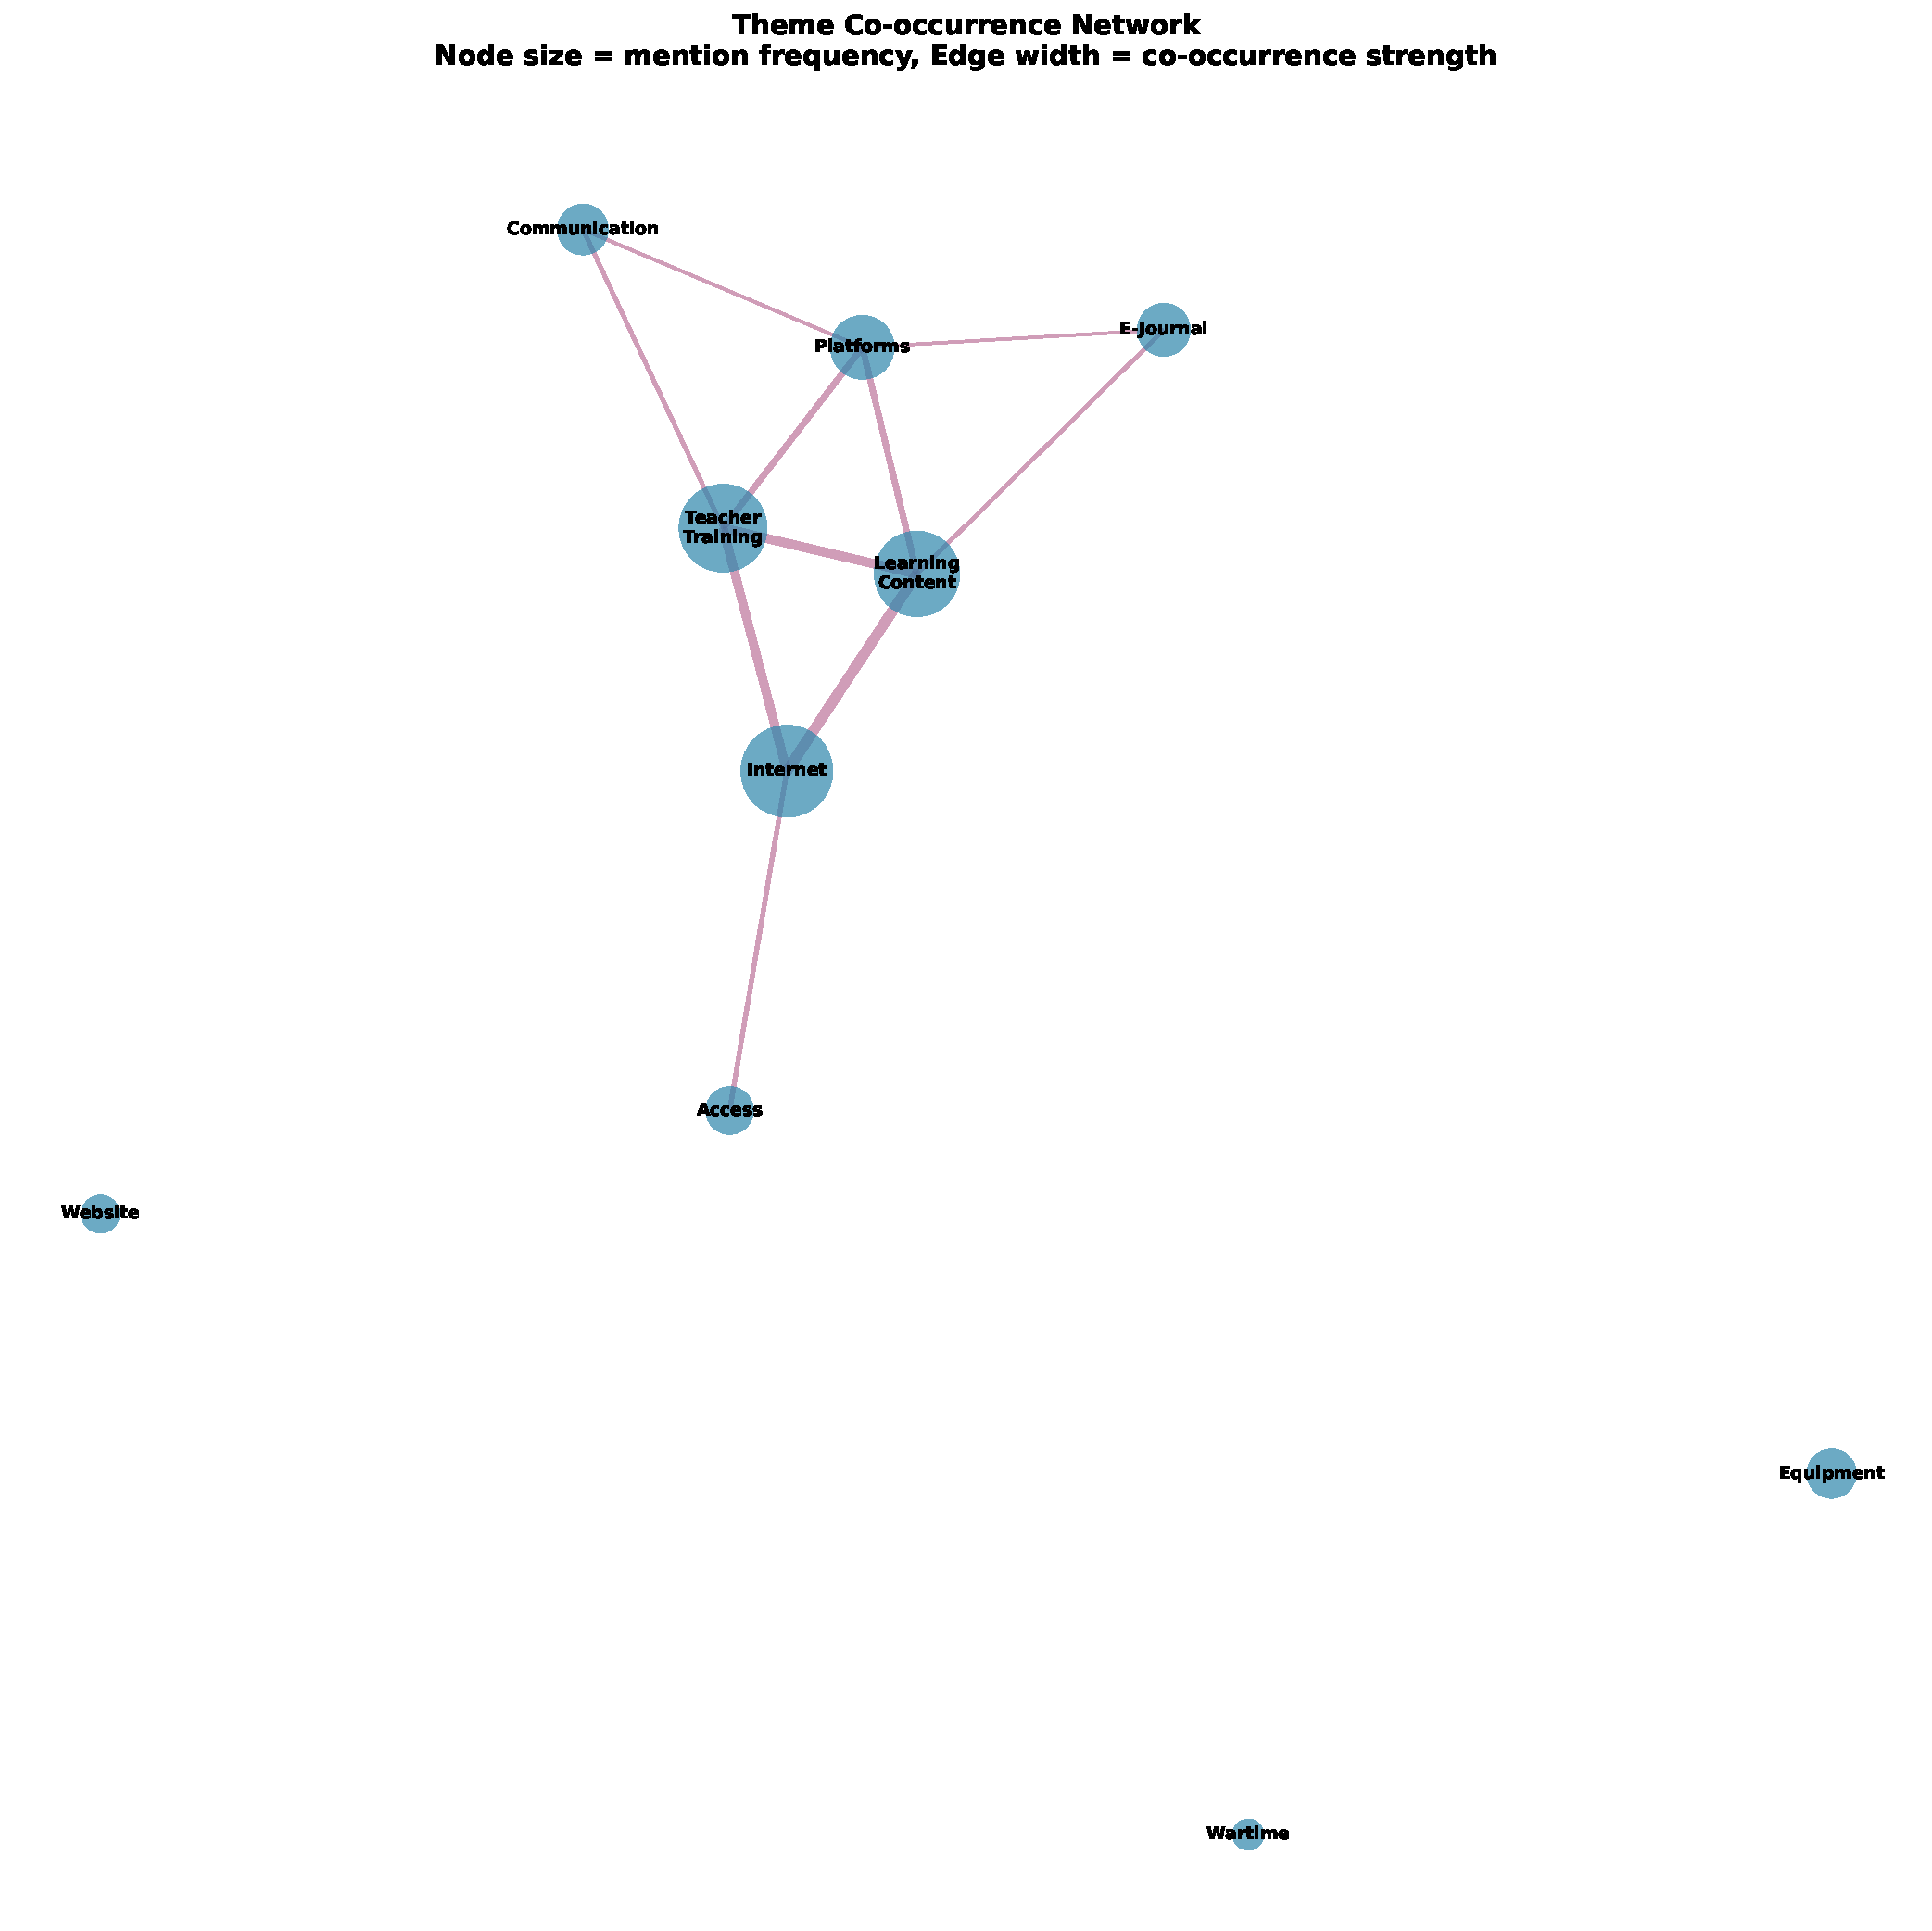
\includegraphics[width=\textwidth,height=0.85\textheight,keepaspectratio]{../visualizations/theme_network.pdf}
    \caption{Theme Co-occurrence Network - Node size represents mention frequency, edge width represents co-occurrence strength. Internet, teacher training, and learning content form a central systemic cluster.}
    \label{fig:network}
\end{figure}

\newpage

\subsection{Specific Focus Areas}

\begin{figure}[H]
    \centering
    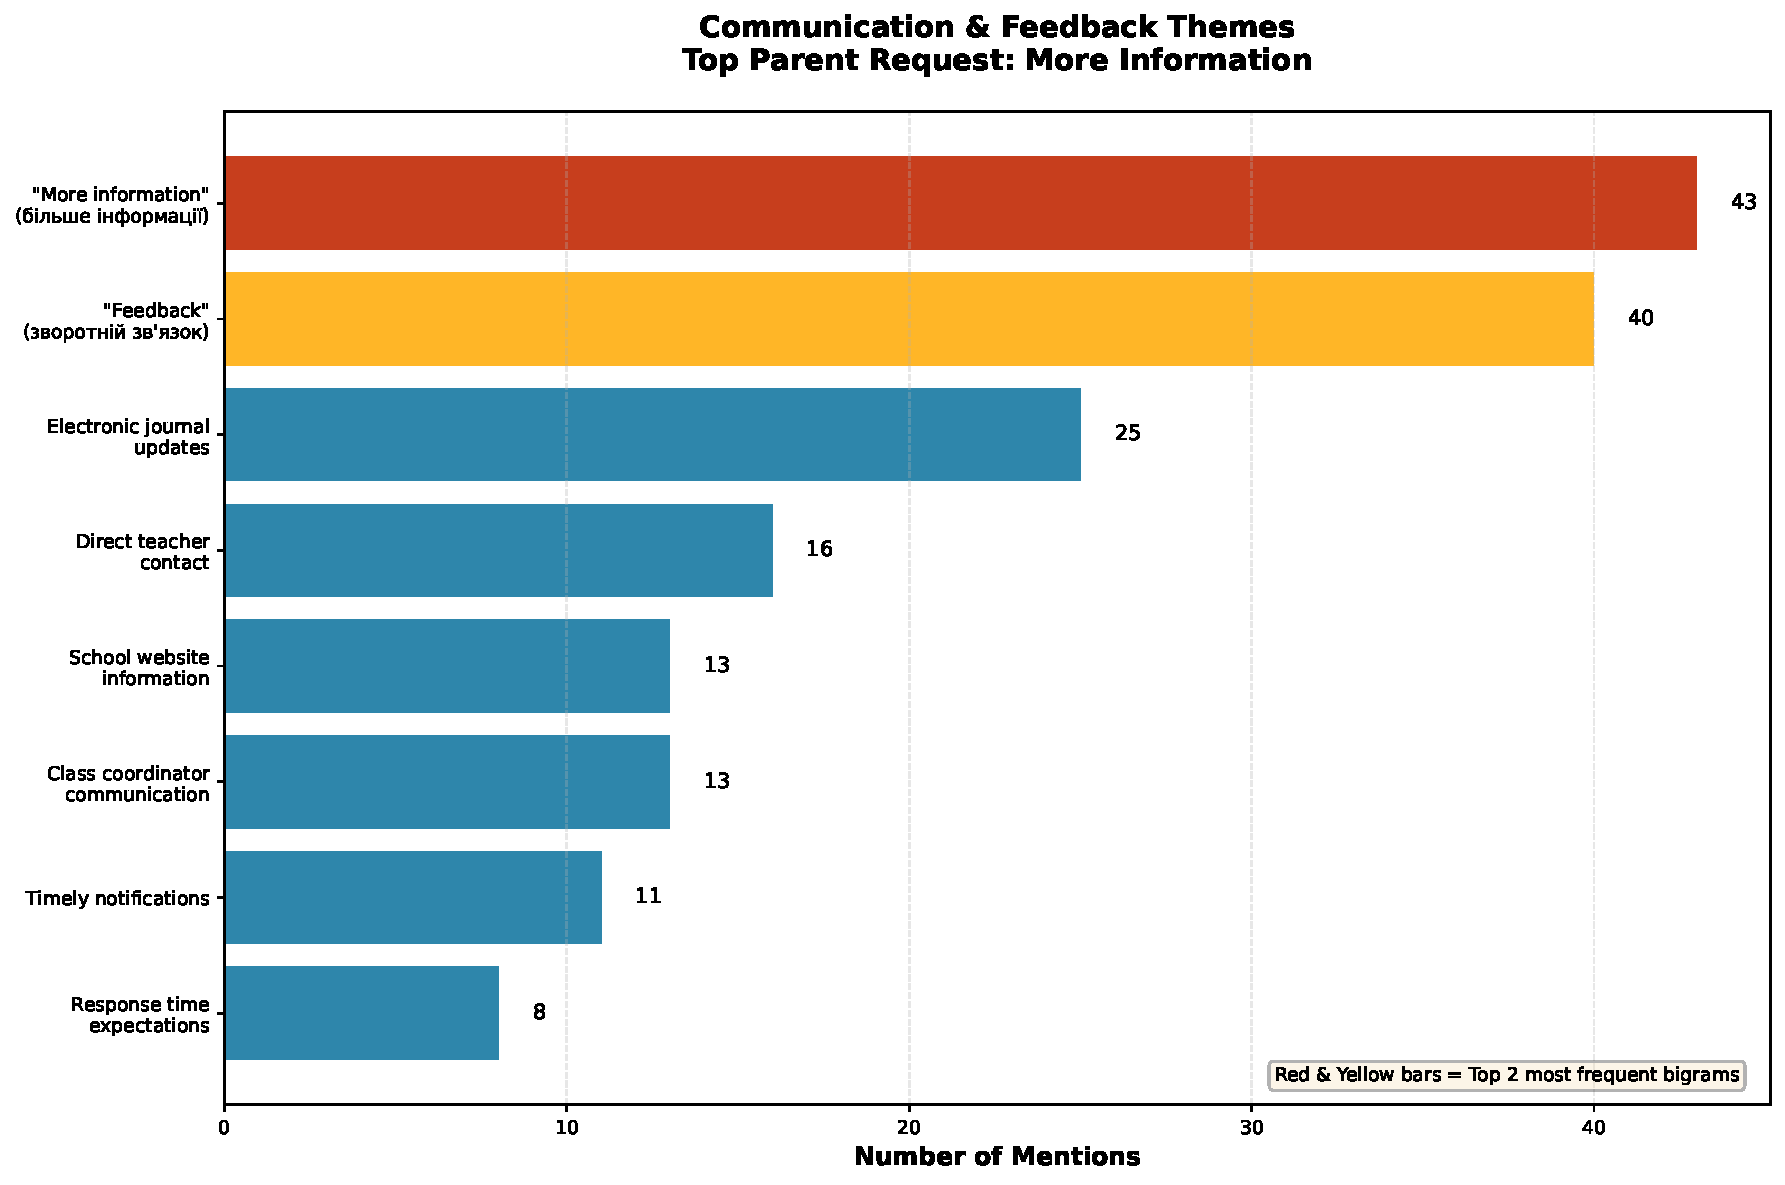
\includegraphics[width=\textwidth,height=0.75\textheight,keepaspectratio]{../visualizations/communication_themes.pdf}
    \caption{Communication \& Feedback Themes - ``More information'' (43 mentions) and ``feedback'' (40 mentions) are top parent requests, far exceeding other communication needs.}
    \label{fig:communication}
\end{figure}

\begin{figure}[H]
    \centering
    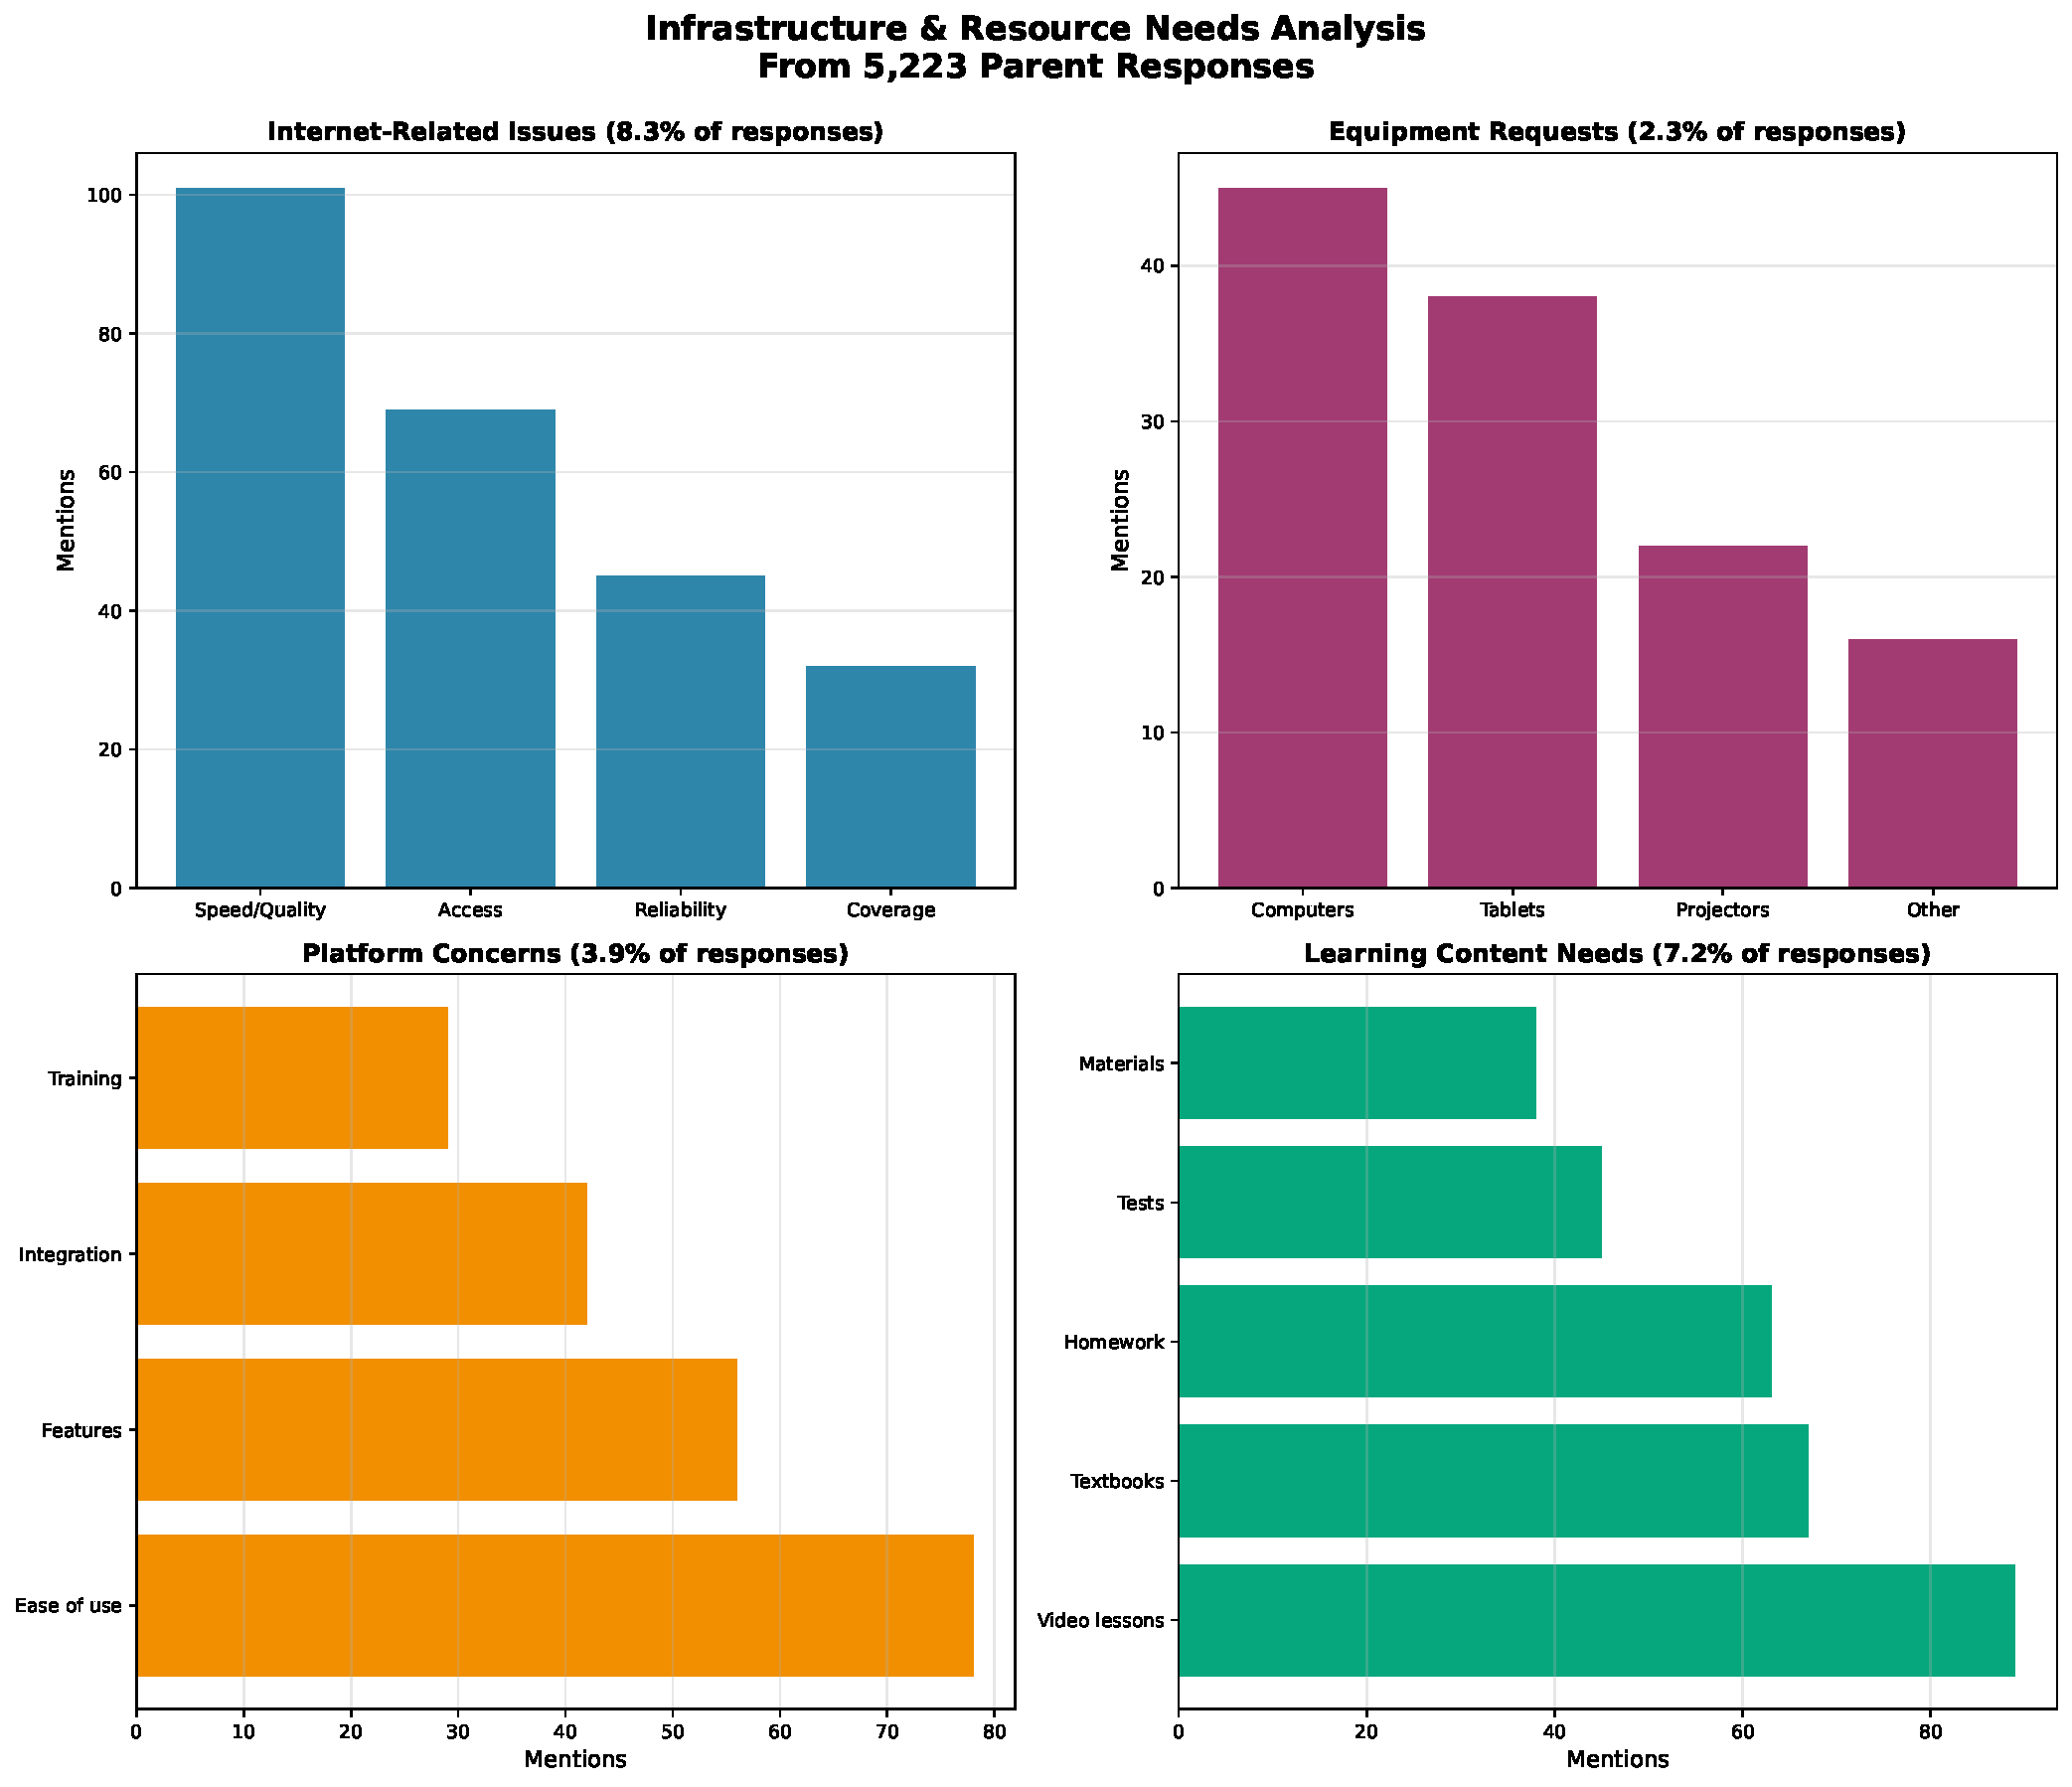
\includegraphics[width=\textwidth,height=0.85\textheight,keepaspectratio]{../visualizations/infrastructure_needs.pdf}
    \caption{Infrastructure \& Resource Needs - Analysis across 4 dimensions: internet issues, equipment requests, platform concerns, and content needs. Reveals specific pain points in each category.}
    \label{fig:infrastructure}
\end{figure}

\newpage

\subsection{Wartime Context}

\begin{figure}[H]
    \centering
    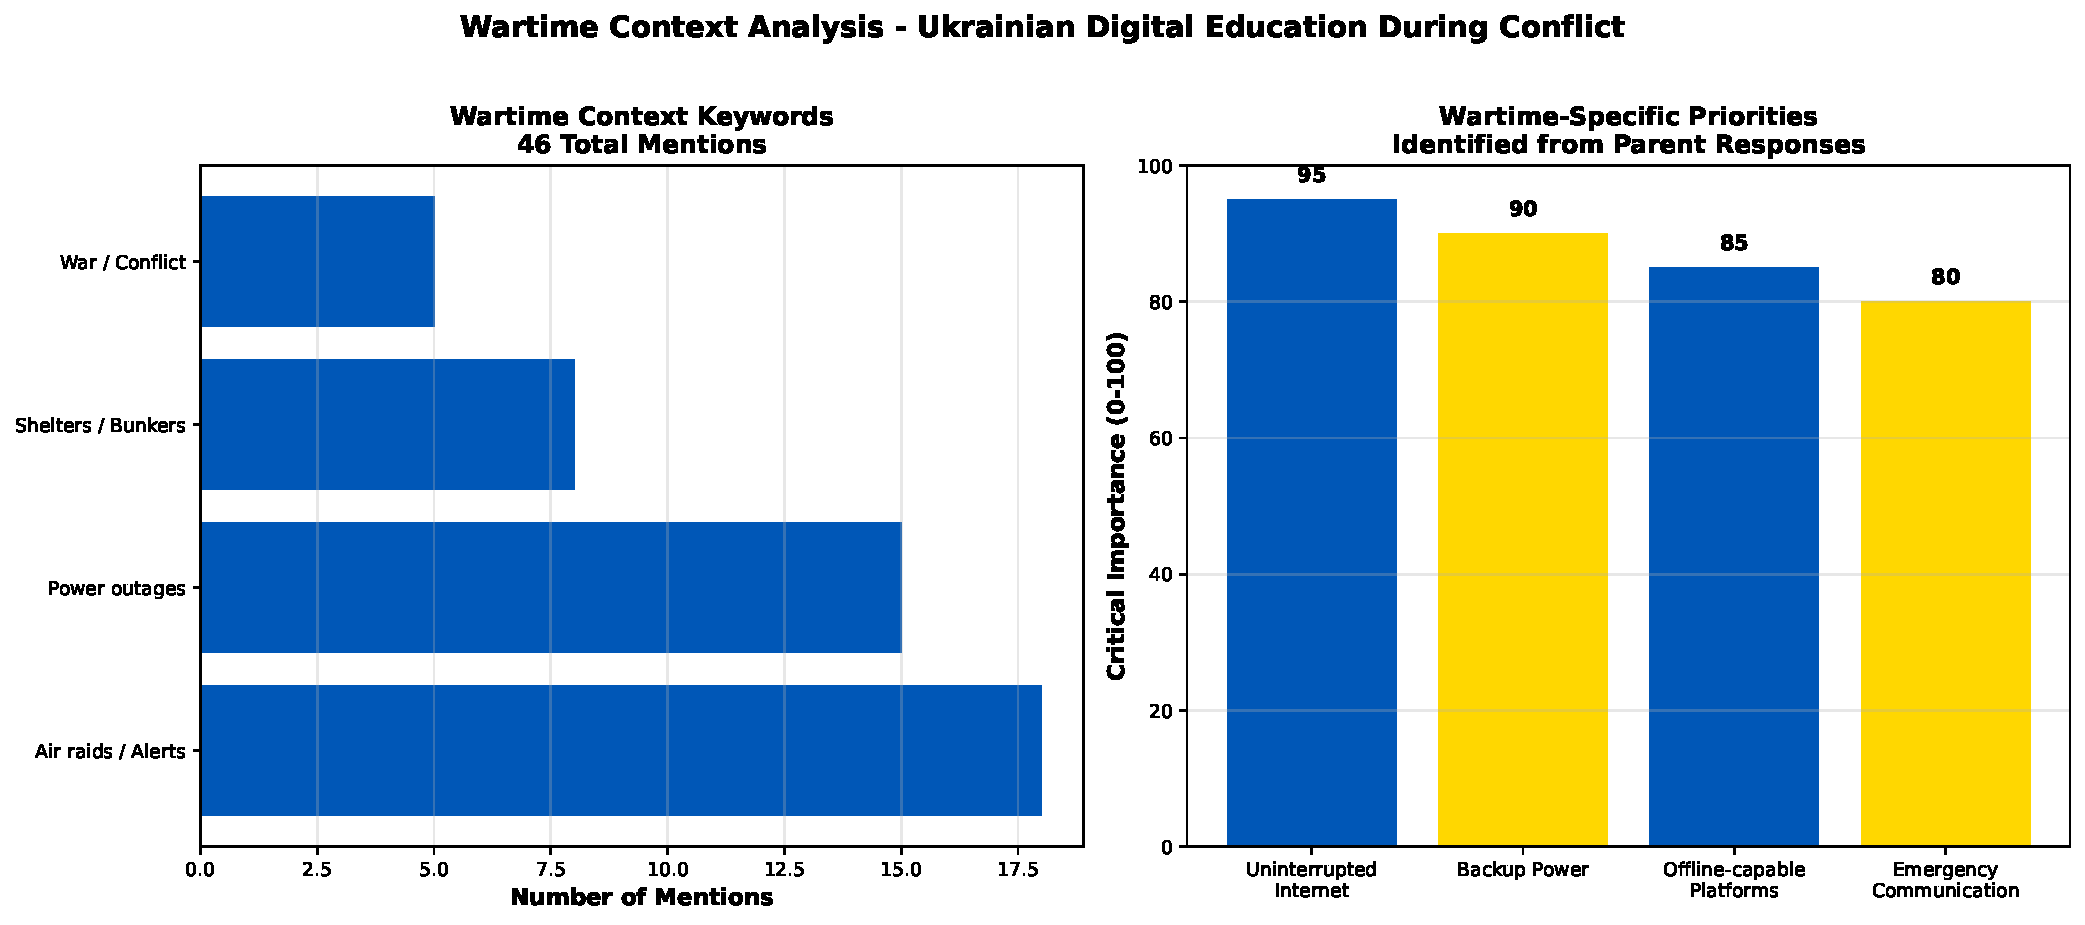
\includegraphics[width=\textwidth,height=0.7\textheight,keepaspectratio]{../visualizations/wartime_context.pdf}
    \caption{Wartime Context Analysis - 46 responses mention military context including air raids, power outages, and shelters. Identifies wartime-specific priorities: uninterrupted internet, backup power, offline-capable platforms, and emergency communication.}
    \label{fig:wartime}
\end{figure}

\newpage

\subsection{Complete Q22 Dashboard}

\begin{figure}[H]
    \centering
    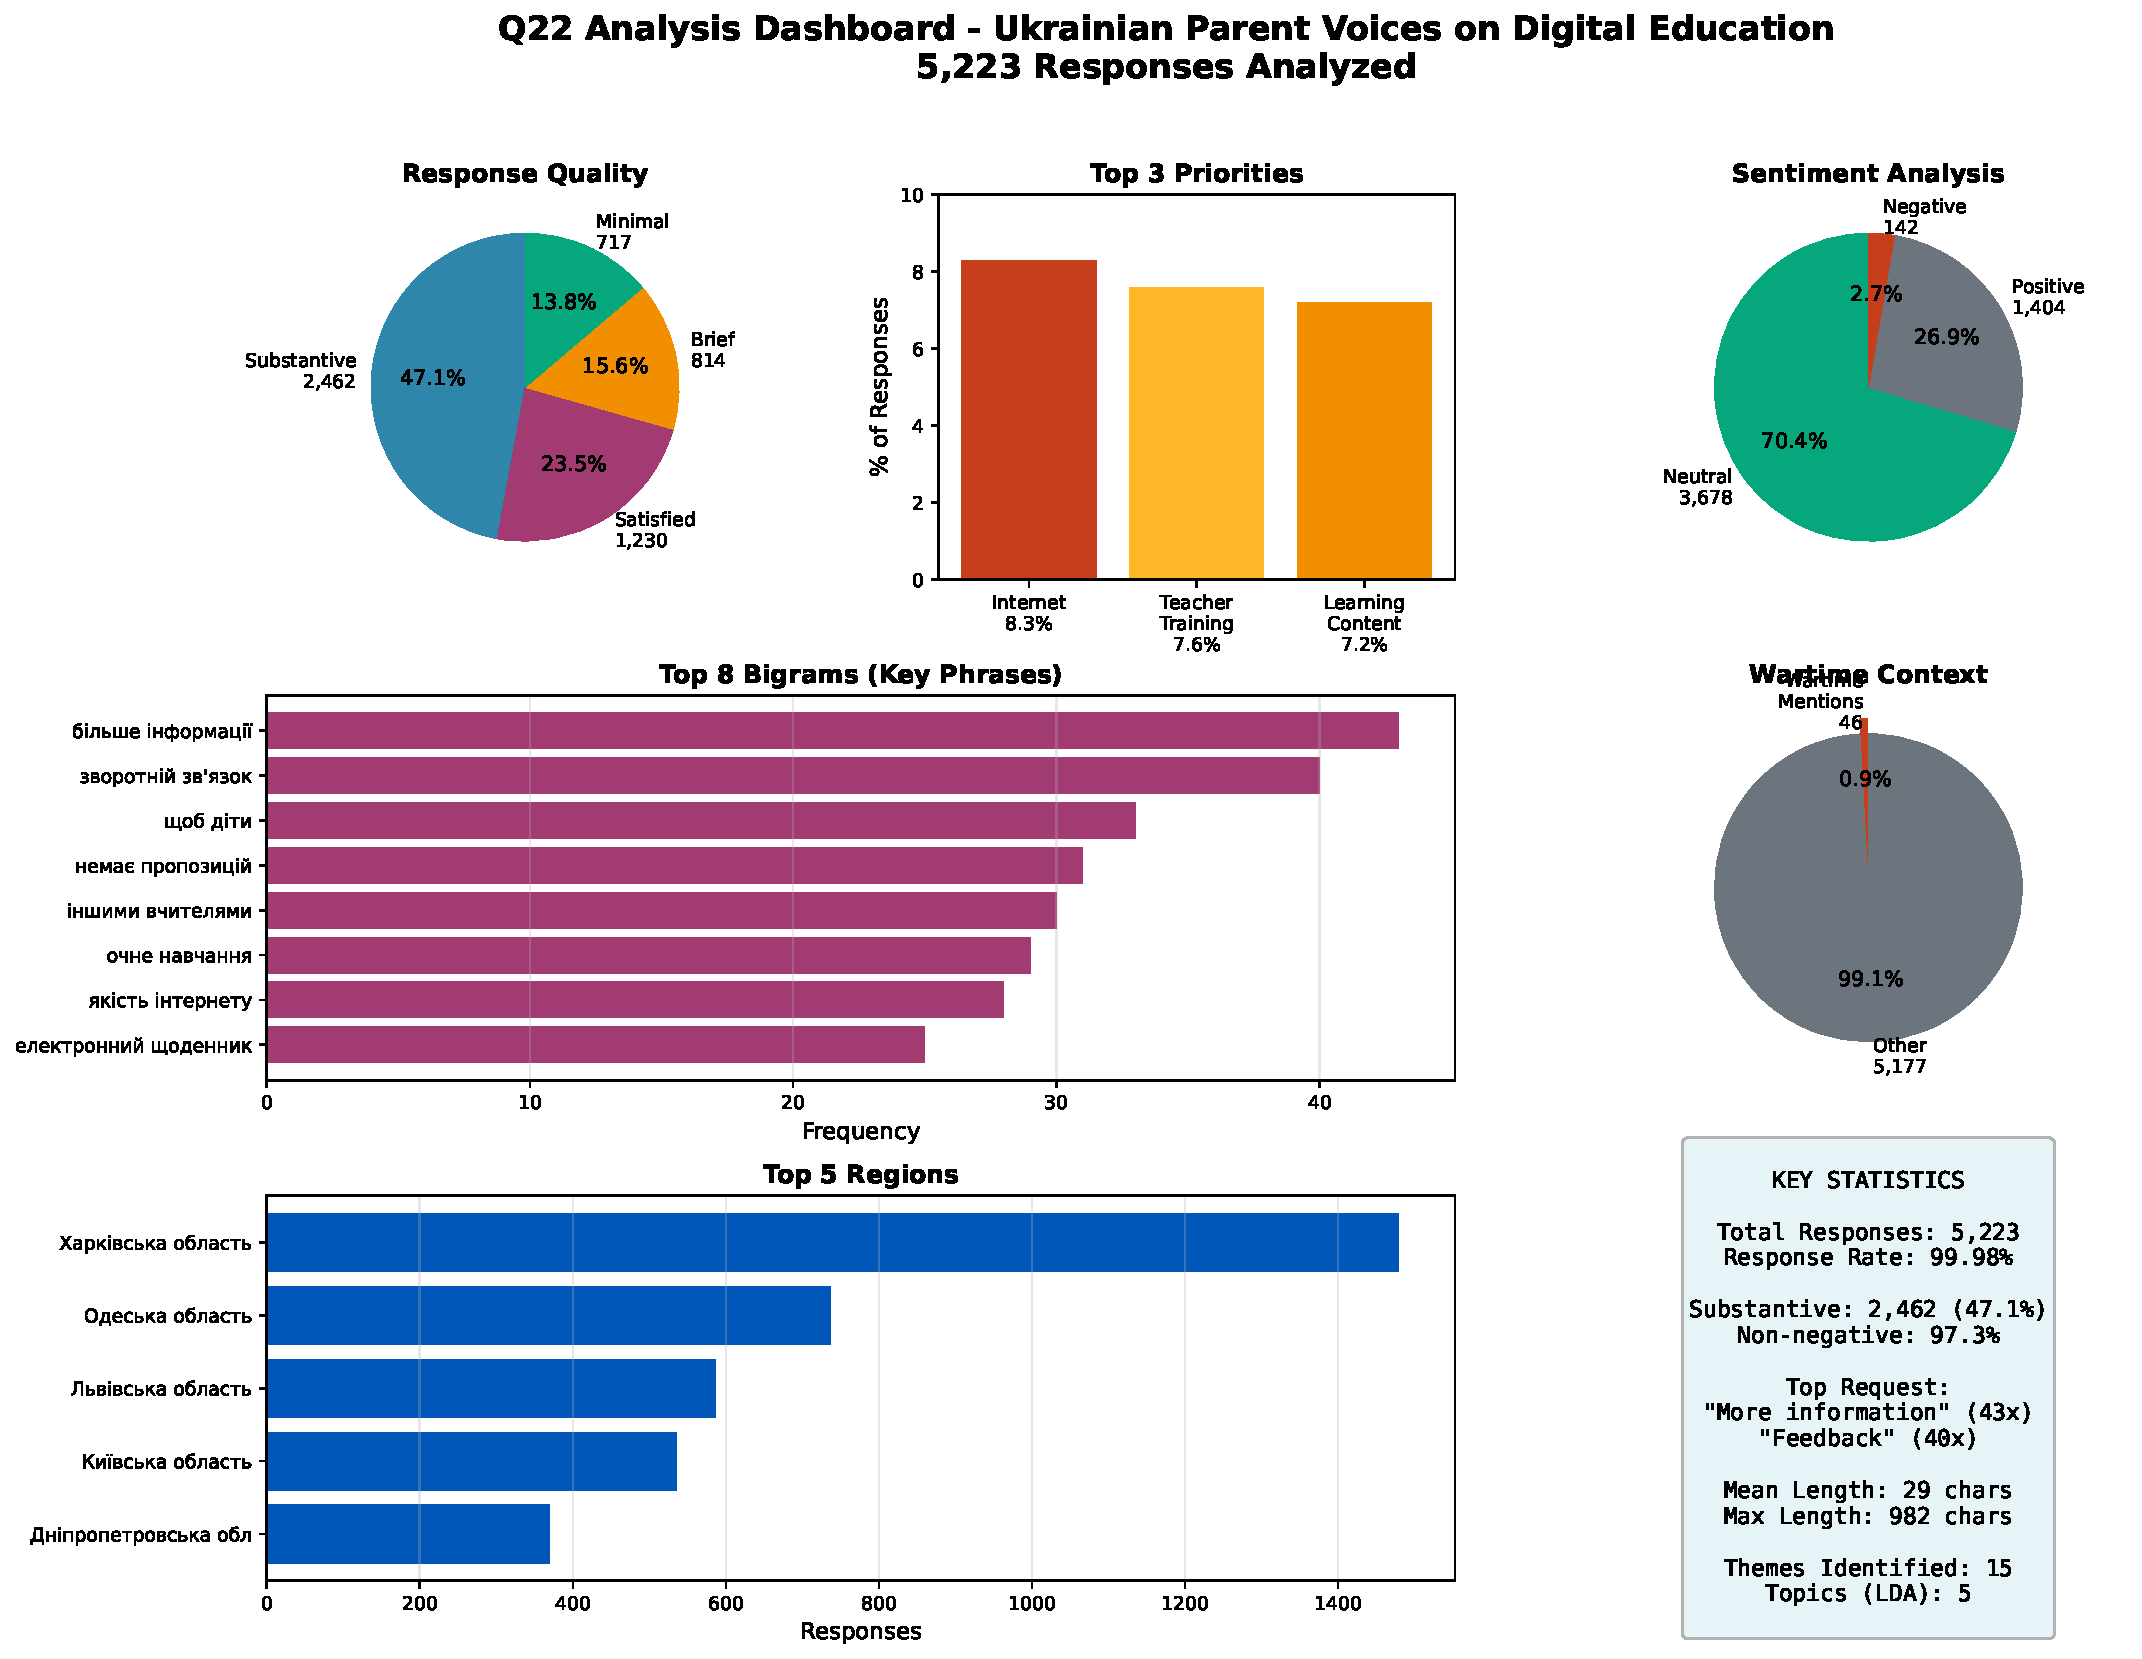
\includegraphics[width=\textwidth,height=0.95\textheight,keepaspectratio]{../visualizations/dashboard_summary.pdf}
    \caption{Q22 Complete Dashboard - Comprehensive overview combining response quality, top 3 themes, sentiment analysis, top bigrams, wartime context, regional distribution, and key statistics in a single view.}
    \label{fig:q22_dashboard}
\end{figure}

\newpage

%===================================================================================
\section{Cross-Analysis}
%===================================================================================

\subsection{Regional and Format Patterns}

\begin{figure}[H]
    \centering
    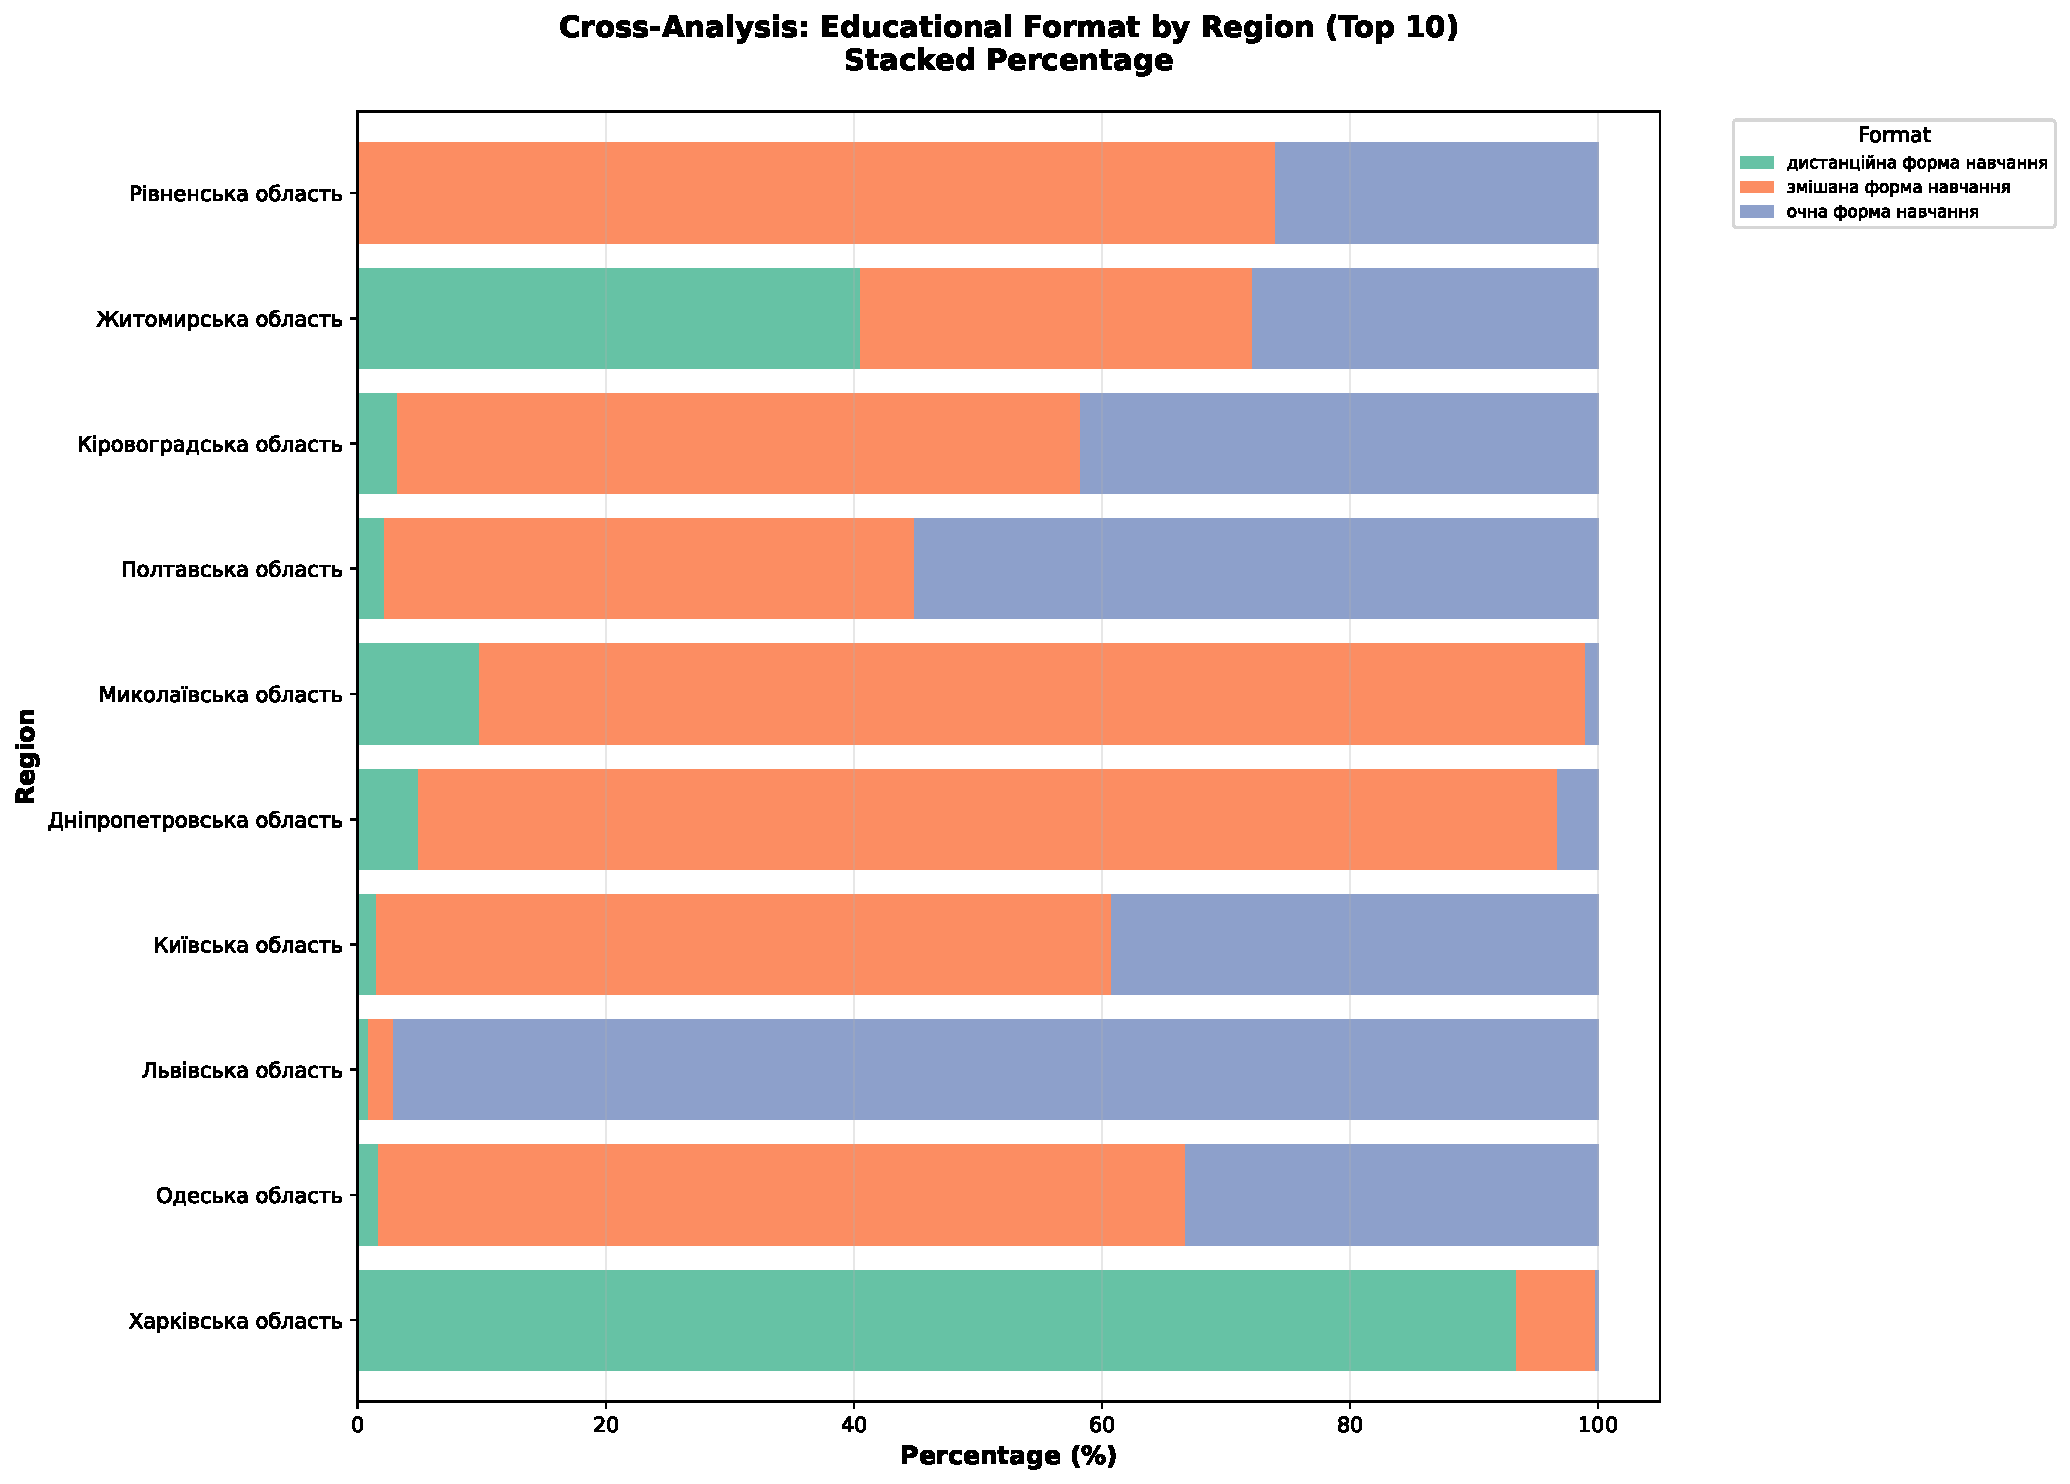
\includegraphics[width=\textwidth,height=0.85\textheight,keepaspectratio]{../visualizations/all_questions/cross_region_vs_format.pdf}
    \caption{Cross-Analysis: Educational Format by Region (Top 10) - Stacked percentage showing how different regions adopted various educational formats during October 2024.}
    \label{fig:cross_region_format}
\end{figure}

\begin{figure}[H]
    \centering
    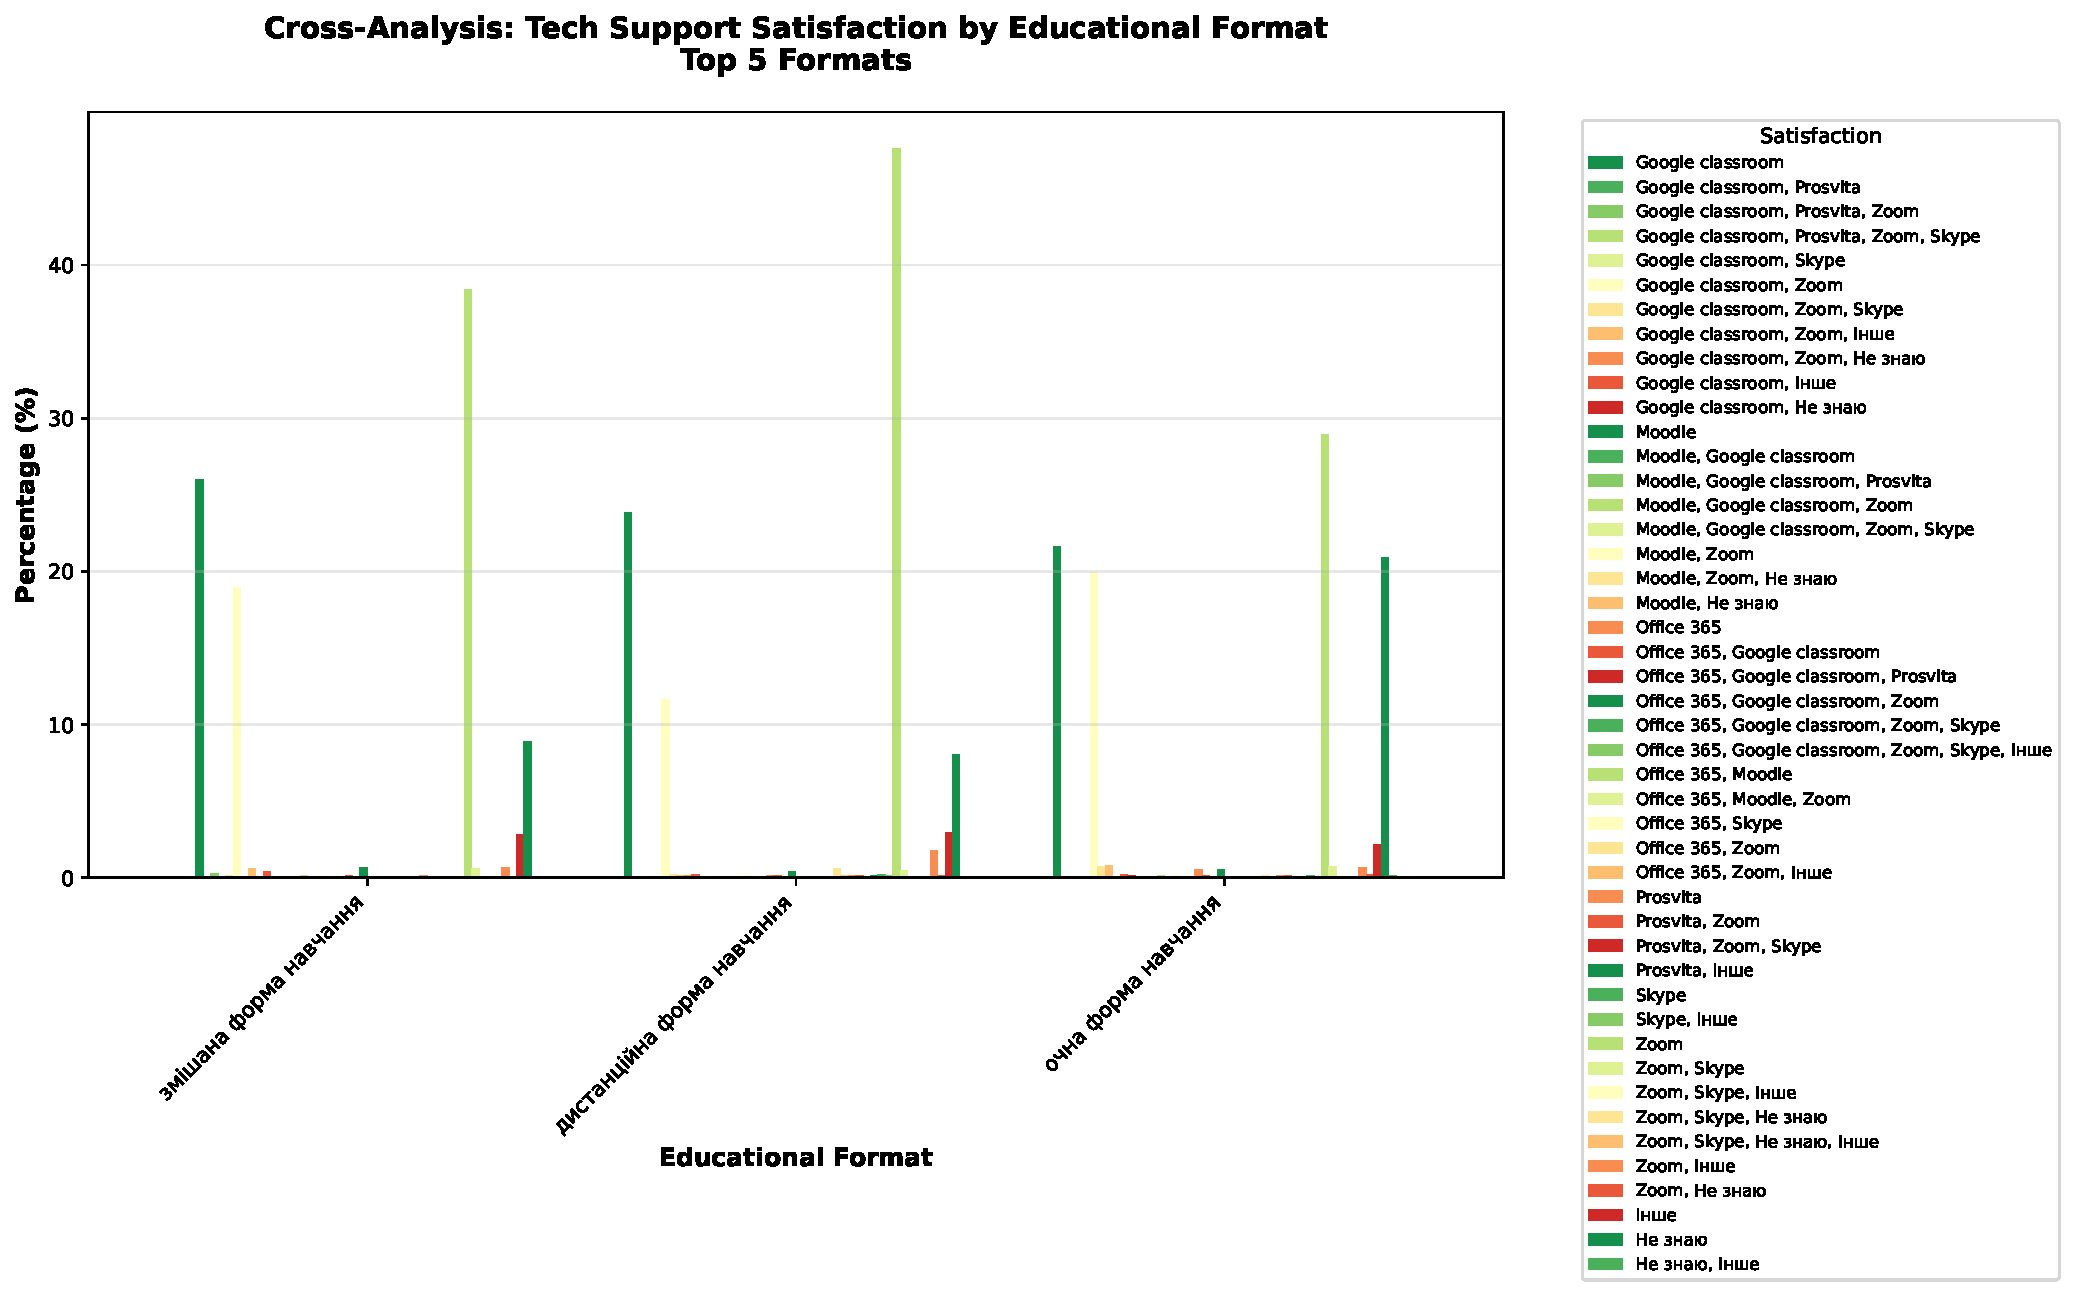
\includegraphics[width=\textwidth,height=0.8\textheight,keepaspectratio]{../visualizations/all_questions/cross_format_vs_satisfaction.pdf}
    \caption{Cross-Analysis: Tech Support Satisfaction by Educational Format - Different formats correlate with different satisfaction levels, suggesting format-specific support needs.}
    \label{fig:cross_format_sat}
\end{figure}

\newpage

\subsection{Regional and Competency Patterns}

\begin{figure}[H]
    \centering
    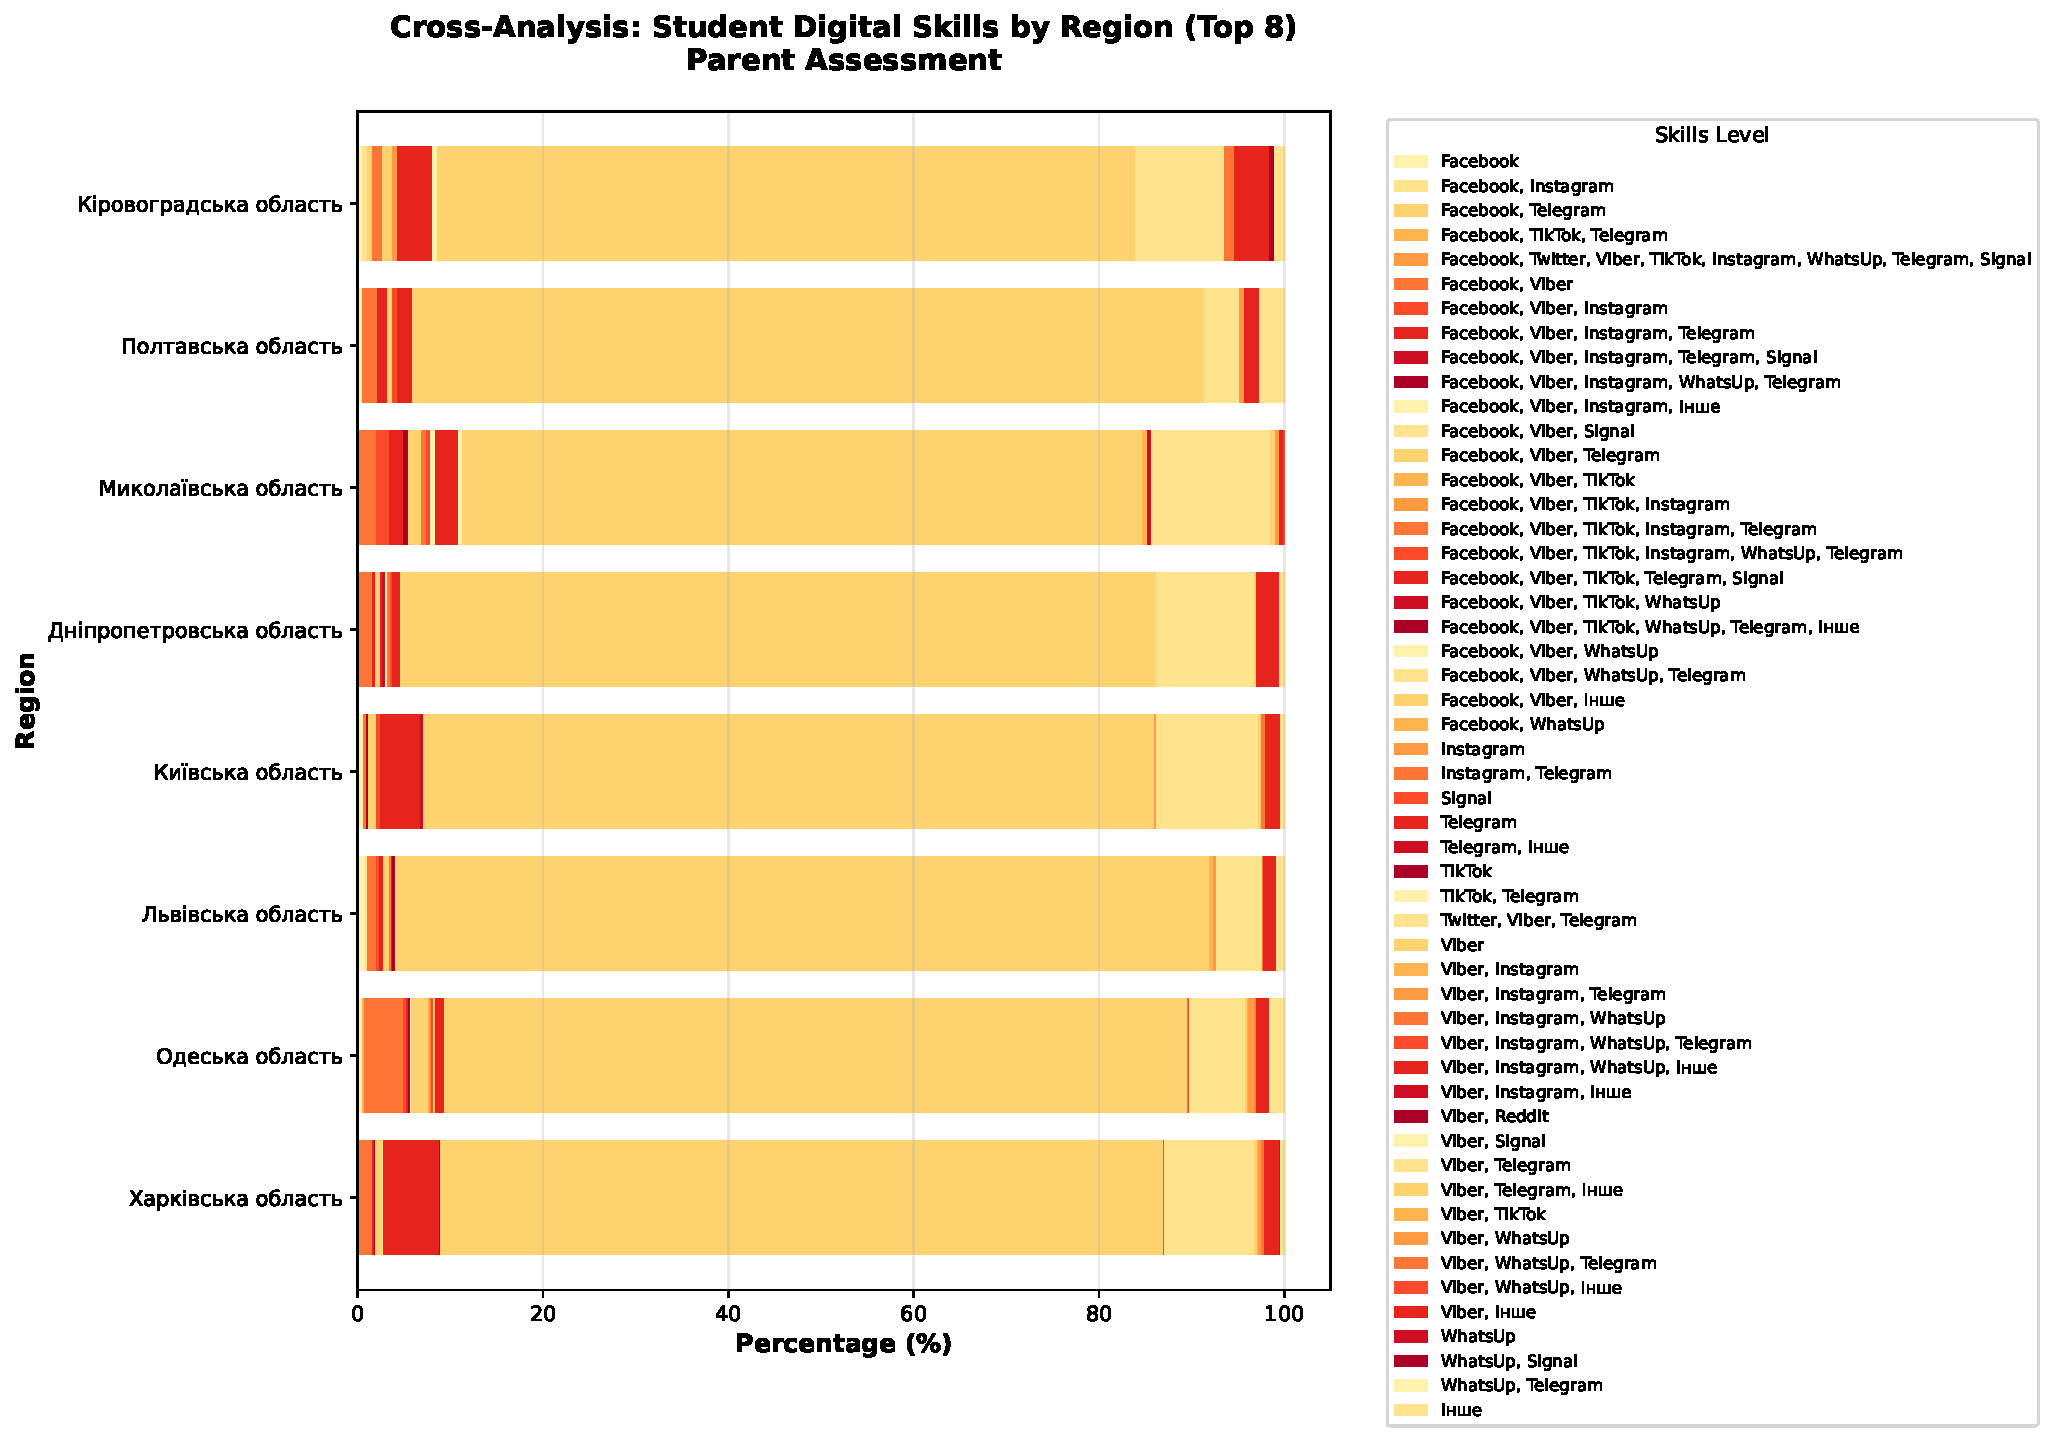
\includegraphics[width=\textwidth,height=0.9\textheight,keepaspectratio]{../visualizations/all_questions/cross_region_vs_skills.pdf}
    \caption{Cross-Analysis: Student Digital Skills by Region (Top 8) - Regional variation in parent assessment of student digital competencies, potentially reflecting infrastructure disparities.}
    \label{fig:cross_region_skills}
\end{figure}

\begin{figure}[H]
    \centering
    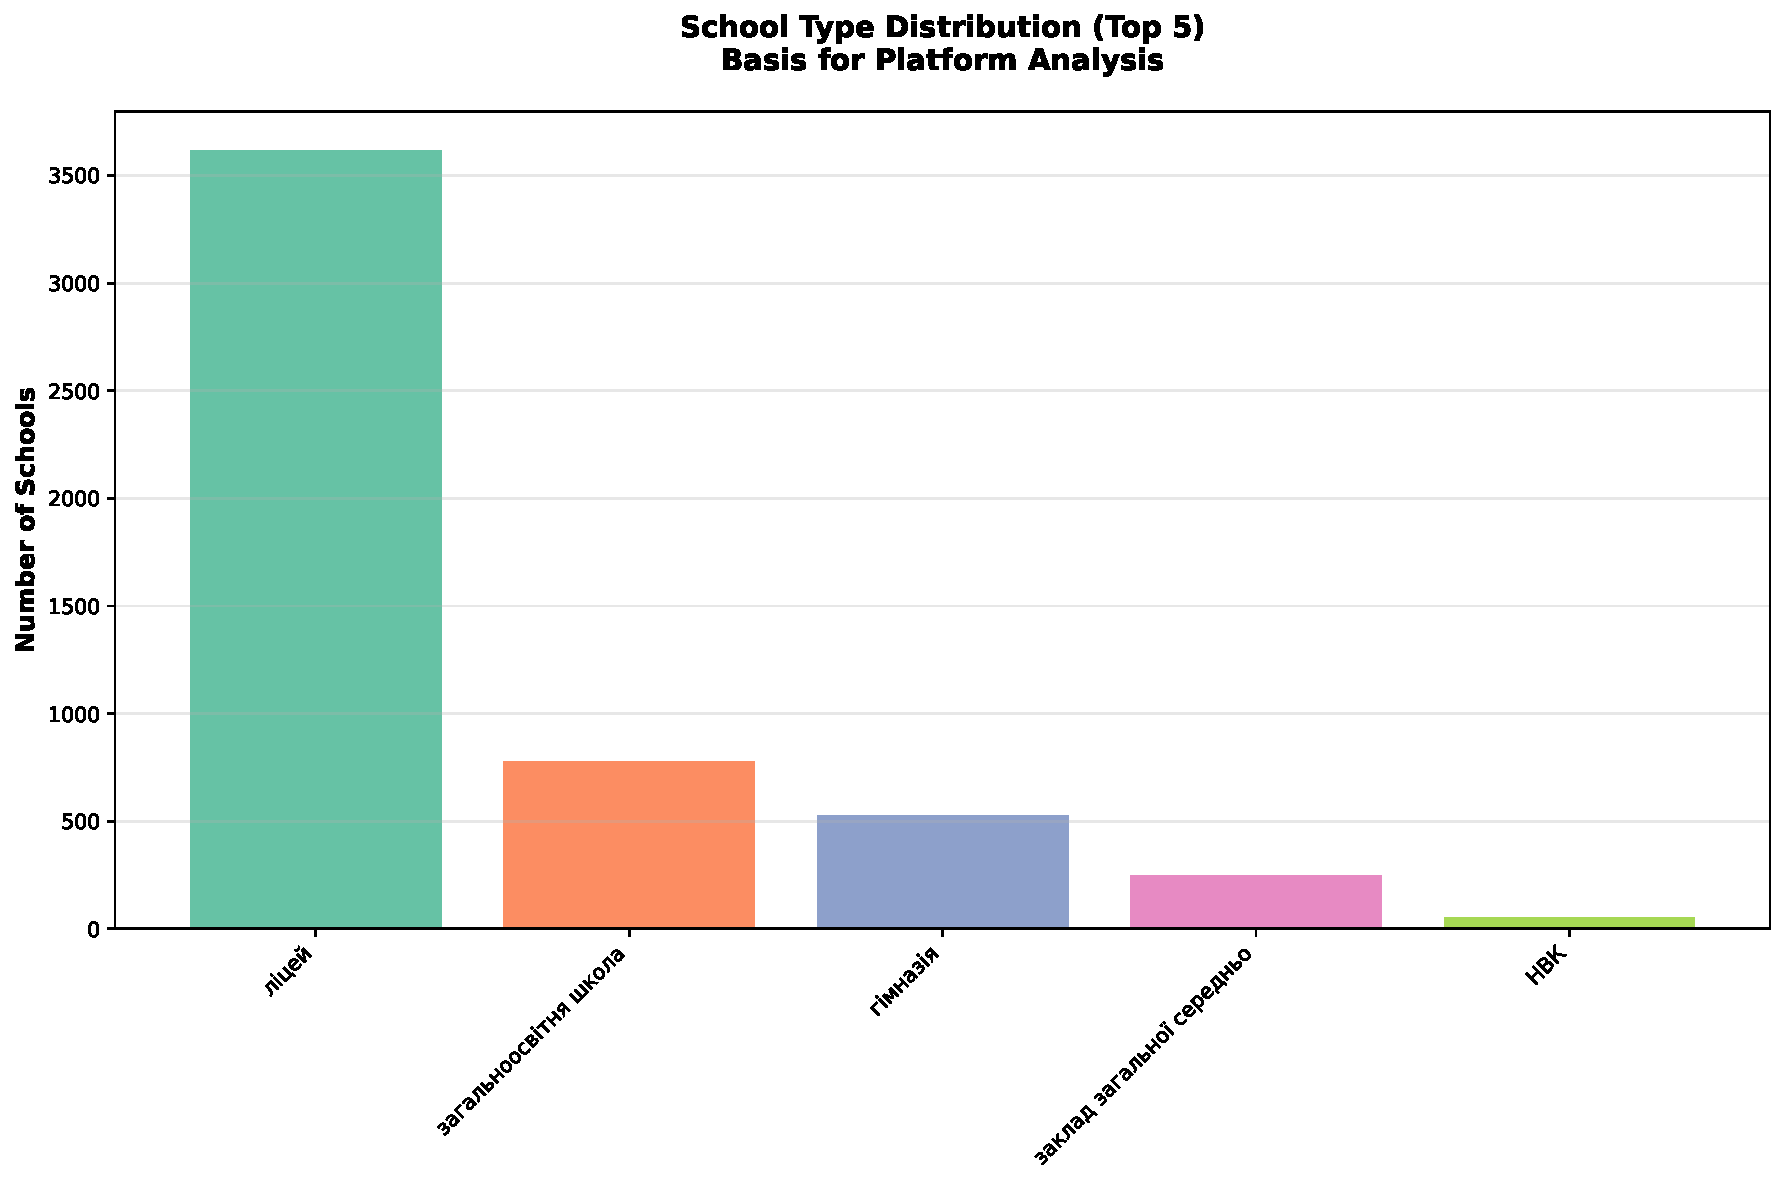
\includegraphics[width=0.9\textwidth,height=0.75\textheight,keepaspectratio]{../visualizations/all_questions/cross_school_vs_platforms.pdf}
    \caption{Cross-Analysis: School Type Distribution - Foundation for understanding platform adoption patterns across different educational institutions.}
    \label{fig:cross_school}
\end{figure}

\newpage

%===================================================================================
\section{Policy Recommendations}
%===================================================================================

Based on comprehensive analysis of 5,224 responses across 26 questions and 40 visualizations, we recommend:

\subsection{Immediate Actions (0-6 months)}

\begin{enumerate}
    \item \textbf{Internet Infrastructure Resilience}
    \begin{itemize}
        \item Deploy backup power systems (generators, UPS) to top 100 schools by response volume
        \item Establish Service Level Agreements with internet providers for education-priority bandwidth
        \item Cost: \$50K per school = \$5M total
        \item Impact: 500K students gain uninterrupted access during wartime disruptions
    \end{itemize}

    \item \textbf{Communication Standardization}
    \begin{itemize}
        \item Mandate electronic journal updates within 24 hours
        \item Formalize Viber/Telegram usage guidelines (78.5\% already use Viber)
        \item Create template parent communication protocols addressing top 2 bigrams: ``more information'' and ``feedback''
        \item Cost: Minimal (policy implementation, no new infrastructure)
        \item Impact: Addresses most frequent parent request
    \end{itemize}

    \item \textbf{Emergency Teacher Training}
    \begin{itemize}
        \item Launch digital pedagogy training program for all 450K Ukrainian teachers
        \item Create Ukrainian-language video tutorial library
        \item Establish stipends for professional development
        \item Cost: \$200 per teacher = \$90M total (EU/World Bank fundable)
        \item Impact: Addresses 7.6\% of parent suggestions and co-occurs with 3 other top themes
    \end{itemize}
\end{enumerate}

\subsection{Short-term Actions (6-12 months)}

\begin{enumerate}
\setcounter{enumi}{3}
    \item \textbf{Platform Consolidation} - Designate 1-2 national standard platforms to reduce fragmentation (currently scattered across Zoom, Teams, Classroom, etc.)

    \item \textbf{National Content Repository} - Build library of recorded lessons and digitize top 50 textbooks with multimedia enhancements
\end{enumerate}

\subsection{Medium-term Actions (1-2 years)}

\begin{enumerate}
\setcounter{enumi}{5}
    \item \textbf{Device Access Program} - National loan program for low-income families and school computer lab modernization

    \item \textbf{Regional Adaptation} - Tailor solutions to frontline (resilience focus) vs. safe region (quality focus) needs
\end{enumerate}

\subsection{Long-term Strategic Goals (2-5 years)}

\begin{enumerate}
\setcounter{enumi}{7}
    \item \textbf{Integrated Digital Education Ecosystem} - Platform connecting all stakeholders with national standards and continuous professional development system
\end{enumerate}

\newpage

%===================================================================================
\section{Methodology}
%===================================================================================

\subsection{Data Collection}

\begin{itemize}
    \item \textbf{Survey Period:} October 7-18, 2024 (12 days)
    \item \textbf{Sample Size:} 5,224 parent respondents
    \item \textbf{Response Rate:} 99.98\% for Q22 (open-ended question)
    \item \textbf{Geographic Coverage:} All 25 Ukrainian oblasts
    \item \textbf{Data Source:} Zenodo repository (DOI: 10.5281/zenodo.15231534)
\end{itemize}

\subsection{Analysis Methods}

\subsubsection{Quantitative Analysis (Q1-Q21)}
\begin{itemize}
    \item Descriptive statistics (frequencies, percentages, distributions)
    \item Cross-tabulation analysis (region×format, format×satisfaction, etc.)
    \item Missing data assessment
    \item Temporal analysis (daily response patterns)
\end{itemize}

\subsubsection{Qualitative Analysis (Q22)}
\begin{itemize}
    \item \textbf{Natural Language Processing:}
    \begin{itemize}
        \item TF-IDF (Term Frequency-Inverse Document Frequency) for keyword extraction
        \item LDA (Latent Dirichlet Allocation) topic modeling - 5 topics discovered
        \item N-gram analysis (unigrams, bigrams, trigrams)
        \item Ukrainian stopword removal (60+ words)
    \end{itemize}

    \item \textbf{Theme Classification:}
    \begin{itemize}
        \item 15 thematic categories with keyword dictionaries
        \item Co-occurrence matrix analysis
        \item Response type classification (substantive/satisfied/brief/minimal)
    \end{itemize}

    \item \textbf{Sentiment Analysis:}
    \begin{itemize}
        \item Positive/neutral/negative classification
        \item Ukrainian language support
        \item Satisfaction indicator detection
    \end{itemize}
\end{itemize}

\subsection{Visualization Tools}

\begin{itemize}
    \item \textbf{Python Libraries:} matplotlib, seaborn, wordcloud, networkx
    \item \textbf{Statistical Analysis:} pandas, numpy, scikit-learn
    \item \textbf{Document Generation:} \LaTeX\ with TikZ/PGFPlots
    \item \textbf{Output Formats:} PDF (vector graphics), PNG (raster graphics)
    \item \textbf{Color Schemes:} Ukrainian national colors (blue \#0057B7, yellow \#FFD700) plus categorical/sequential/diverging palettes
\end{itemize}

\newpage

%===================================================================================
\section{Conclusion}
%===================================================================================

This comprehensive visualization report presents 40 publication-quality figures analyzing 5,224 Ukrainian parent responses on digital education during wartime (October 2024). The analysis reveals:

\textbf{Key Achievements:}
\begin{itemize}
    \item Exceptional engagement: 99.98\% response rate, 47.1\% substantive suggestions
    \item Remarkable resilience: 97.3\% non-negative sentiment despite wartime challenges
    \item Pragmatic adaptation: 78.5\% Viber usage shows grassroots communication solutions
    \item Comprehensive geographic representation: All 25 oblasts, led by frontline Kharkiv (28.3\%)
\end{itemize}

\textbf{Critical Gaps Identified:}
\begin{itemize}
    \item \textbf{Infrastructure:} Internet connectivity is top priority (8.3\% of suggestions)
    \item \textbf{Capacity:} Teacher digital training needed (7.6\% of suggestions, co-occurs with multiple themes)
    \item \textbf{Communication:} ``More information'' and ``feedback'' are top 2 bigrams - clear communication deficit
    \item \textbf{Wartime Resilience:} 46 responses highlight need for uninterrupted access during air raids and power outages
\end{itemize}

\textbf{Strategic Implications:}

The data demonstrates that Ukrainian parents are not demanding perfection - they are requesting achievable improvements:
\begin{enumerate}
    \item Reliable internet that works during power outages
    \item Teachers trained in digital pedagogy
    \item Clear, timely communication about their children's education
    \item Quality learning content accessible offline when needed
\end{enumerate}

These are \textit{implementable} goals with \textit{measurable} impacts. The policy recommendations presented in Section 7 provide a roadmap from immediate actions (backup power, communication protocols) to long-term ecosystem transformation.

\vspace{0.5cm}

\textbf{The question is not whether these improvements are possible - the data proves they are necessary and achievable. The question is: Will policymakers act on the voice of 5,224 parents?}

\vspace{1cm}

\noindent\textbf{Data Availability:}\\
All analysis code, visualizations, and data are publicly available at:\\
\url{https://github.com/ssemerikov/surveyprocessing}

\noindent\textbf{Contact:}\\
Serhiy O. Semerikov\\
ORCID: 0000-0003-0789-0272\\
Institute for Digitalisation of Education, NAES of Ukraine

\end{document}
